%============================================================
% BAB 3: DESAIN SISTEM
%============================================================
\chapter{DESAIN SISTEM}

Bab ini menguraikan rancangan penelitian, deskripsi solusi dan arsitektur \textit{Modular Monolithic} 10 modul (termasuk Modul \texttt{AI / MCP Assistant}), alur proses bisnis, pemodelan fungsional dan aliran data (\textit{Use Case} serta DFD), rancangan basis data (ERD), rancangan evaluasi sistem beserta \textit{flowchart} evaluasi, dan lini masa pengerjaan Proyek Akhir.

\section{RANCANGAN PENELITIAN}
\label{sec:rancangan_penelitian}

Penelitian ini dilaksanakan menggunakan pendekatan rekayasa perangkat lunak iteratif berbasis kerangka kerja \textbf{Scrum} yang dibagi ke dalam empat siklus \textit{sprint}~\cite{schwaber2020}. Tahapan rancangan penelitian disusun secara berurutan sebagai berikut:
\begin{enumerate}[label=\arabic*., leftmargin=*]
  \item \textbf{Analisis Masalah dan Audit Sistem Lama:} Mengidentifikasi kendala operasional pengelolaan rumah kost multi-gedung serta mengaudit struktur kode dan skema 34 tabel domain pada empat proyek akhir sebelumnya untuk memetakan akar masalah \textit{tight coupling}, pembengkakan skema, dan ketiadaan isolasi multi-gedung.
  \item \textbf{Perancangan Arsitektur dan Pemodelan Sistem:} Merancang arsitektur baru berbasis \textit{Modular Monolith} NestJS dengan 10 modul terenkapsulasi (4 \textit{core} + 6 \textit{opsional} termasuk Modul \texttt{AI / MCP Assistant}), antarmuka Flutter Web berbasis \textit{Clean Architecture}, alur proses bisnis (BPMN), pemodelan \textit{Use Case}, DFD Level 0--1, serta penyederhanaan basis data menjadi 21 tabel domain tanpa \textit{Foreign Key} lintas modul.
  \item \textbf{Implementasi Bertahap Berbasis Scrum (4 \textit{Sprint}):}
    \begin{enumerate}[label=\alph*., leftmargin=*]
      \item \textit{Sprint 1 (Fondasi Core \& Keamanan):} Konfigurasi Docker, PostgreSQL, integrasi Keycloak OIDC, dan implementasi 4 modul \textit{core} (\texttt{Auth}, \texttt{Building}, \texttt{Room}, \texttt{Lease}).
      \item \textit{Sprint 2 (Finansial \& Pembayaran):} Implementasi modul \texttt{Finance} (tagihan otomatis, \textit{Two-Phase Invoicing}, denda, pengeluaran) dan integrasi Midtrans SNAP dengan verifikasi \textit{webhook} idempoten.
      \item \textit{Sprint 3 (Operasional Gedung \& Notifikasi):} Implementasi modul opsional \texttt{Maintenance}, \texttt{Inventory}, \texttt{Guest}, dan \texttt{Notification} serta antarmuka Flutter Web untuk 3 peran.
      \item \textit{Sprint 4 (Modul AI \& Penguatan Sistem):} Implementasi modul \texttt{AI / MCP Assistant} (\textit{read-only} melalui \textit{Module Gateway}), pemantapan sakelar modul per gedung, dan persiapan uji coba.
    \end{enumerate}
  \item \textbf{Evaluasi dan Pengujian Sistem:} Menjalankan lima skenario evaluasi terukur (pengujian \textit{black-box} fungsional, pengujian kombinasi modularitas, pengujian isolasi \textit{multi-tenant}, pengujian idempotensi \textit{webhook} Midtrans, serta pengujian akurasi dan keamanan \textit{read-only} Modul AI) sebagaimana dirinci pada Subbab~\ref{sec:rancangan_evaluasi}.
\end{enumerate}

\section{DESKRIPSI SOLUSI DAN ARSITEKTUR SISTEM}
\label{sec:deskripsi_solusi}

\subsection{Deskripsi Solusi}

Berdasarkan permasalahan yang diuraikan pada Bab~I, solusi yang diusulkan adalah membangun ulang sistem manajemen rumah kost menjadi satu aplikasi web yang dapat melayani banyak gedung sekaligus. Sistem lama berasal dari empat proposal terpisah yang masing-masing menangani satu bagian, yaitu penghuni dan tamu, kamar dan reservasi, keuangan, serta operasional~\cite{rasyidatur2025,roihanah2025,rizal2025,bagus2025}. Keempatnya tidak punya aturan bersama dan hanya dapat dipakai untuk satu gedung. Pada proyek akhir ini, keempat bagian tersebut disatukan ke dalam satu backend dengan batas modul yang jelas, satu basis data, dan satu aplikasi antarmuka untuk tiga peran pengguna: pemilik, pengelola, dan penghuni.

Solusi ini menjawab permasalahan pada Bab~I melalui enam hal berikut:
\begin{enumerate}[label=\arabic*., leftmargin=*]
  \item \textbf{Satu sistem untuk banyak gedung.} Pemilik dapat mendaftarkan beberapa gedung pada satu instalasi sistem. Setiap baris data operasional diberi penanda gedung (\texttt{building\_id}), sehingga pengelola hanya melihat data gedung yang ditugaskan kepadanya, sedangkan pemilik dapat melihat ringkasan seluruh gedung miliknya. Pemilik tidak perlu memasang server atau basis data baru setiap kali membuka cabang.
  \item \textbf{Backend dibagi menjadi sepuluh modul yang terpisah tegas.} Backend dibangun dengan NestJS~\cite{nestjs2025} dan dibagi menjadi empat modul \textit{core} (\texttt{Auth}, \texttt{Building}, \texttt{Room}, \texttt{Lease}) serta enam modul \textit{opsional} (\texttt{Finance}, \texttt{Maintenance}, \texttt{Guest}, \texttt{Inventory}, \texttt{Notification}, dan \texttt{AI / MCP Assistant}). Setiap modul hanya mengelola tabel miliknya sendiri. Jika satu modul perlu memicu perubahan di modul lain, misalnya kontrak sewa baru yang harus menghasilkan tagihan, modul tersebut mengirim \textit{event} dan tidak mengakses tabel modul lain secara langsung. Dengan cara ini, kesalahan pada satu modul tidak merembet ke modul lain, dan setiap modul dapat diuji sendiri.
  \item \textbf{Sewa bulanan dengan aturan per gedung.} Sistem hanya melayani sewa dalam satuan bulan penuh. Durasi minimum sewa diatur oleh masing-masing gedung, bukan ditanam di kode, sehingga gedung yang mewajibkan sewa minimal tiga bulan dan gedung yang mengizinkan sewa satu bulan dapat berjalan di sistem yang sama. Sistem juga mengakomodasi kebijakan pemesanan fleksibel (bayar penuh bulan pertama atau uang tanda jadi/DP flat) per gedung melalui pola \textit{Two-Phase Invoicing} tanpa menambah tabel cicilan baru. Untuk mencegah pemesanan ganda, kamar dikunci selama proses pemesanan berlangsung, sehingga dua penghuni tidak dapat menyewa kamar yang sama pada periode yang sama.
  \item \textbf{Tagihan dan pembayaran berjalan otomatis.} Begitu kontrak sewa tercatat, sistem menerbitkan tagihan, dan penghuni dapat membayar melalui Midtrans dengan Virtual Account atau QRIS. Status pembayaran diperbarui otomatis setelah notifikasi dari Midtrans diverifikasi. Pesan tagihan, pengingat jatuh tempo, dan bukti lunas dikirim lewat WhatsApp, serta dilengkapi tombol aksi kirim pengingat manual bagi pengelola. Bagi calon penghuni yang membatalkan pemesanan sebelum tanggal mulai sewa, sistem memfasilitasi pengajuan pengembalian dana (\textit{refund}) semi-manual yang diselesaikan via transfer m-banking pengelola berlampiran bukti transfer resmi.
  \item \textbf{Operasional gedung tercatat di satu tempat.} Penghuni melaporkan kerusakan lewat formulir yang disertai foto, lalu pengelola memverifikasi laporan dan menugaskan teknisi sampai laporan ditutup. Pengelola juga mencatat inventaris tiap kamar, jadwal perawatan rutin, pengeluaran operasional, dan tamu yang berkunjung. Fitur-fitur ini bersifat opsional dan dapat diaktifkan atau dimatikan sesuai kebutuhan masing-masing gedung.
  \item \textbf{Login terpusat dan Modul AI (\texttt{AI / MCP Assistant}).} Autentikasi ditangani Keycloak, termasuk verifikasi email dan lupa kata sandi, sehingga backend cukup memeriksa token yang dibawa setiap permintaan. Selain itu, disertakan satu modul mandiri berbasis \textit{Model Context Protocol} (\texttt{AI / MCP Assistant}) yang terhubung melalui \textit{Module Gateway} untuk menjawab pertanyaan operasional seperti ``berapa kamar kosong di Gedung A bulan ini'' secara \textit{read-only} dan tetap dibatasi oleh hak akses gedung milik penanya.
\end{enumerate}

Antarmuka dibangun dengan Flutter Web dan menerapkan Clean Architecture. Setiap peran mendapat dasbor sendiri: pemilik memantau seluruh gedung, pengelola menangani operasional harian satu gedung, dan penghuni mengurus kamar, tagihan, serta laporan kerusakannya.

Seluruh kemampuan sistem dirangkum menjadi tujuh belas fitur pada Tabel~\ref{tab:daftar_fitur}. Fitur \textit{core} selalu aktif di setiap gedung karena menopang operasi dasar, sedangkan fitur opsional (termasuk Modul \texttt{AI / MCP Assistant}) dapat dinyalakan atau dimatikan per gedung sesuai kebutuhan operasional.

\begin{longtblr}[
  caption = {Daftar Fitur Sistem},
  label = {tab:daftar_fitur}
]{
  width = \textwidth,
  colspec = {Q[c,1.1cm] X[2.6,l] X[1.4,l] Q[c,1.9cm]}
}
  Kode & Nama Fitur & Modul & Sifat \\
  F01 & Autentikasi Pengguna dan Profil & Auth & Core \\
  F02 & Pengaturan Hak Akses Dinamis & Auth & Core \\
  F03 & Manajemen Multi-Gedung & Building & Core \\
  F04 & Kebijakan Konfigurasi Gedung (Durasi, Mode DP \& Refund) & Building & Core \\
  F05 & Master Kamar dan Kapasitas & Room & Core \\
  F06 & Alokasi dan Penempatan Hunian & Lease & Core \\
  F07 & Dasbor Monitoring Hunian & Lease dan Room & Core \\
  F08 & Penagihan Sewa Berkala \& DP (Two-Phase Invoicing) & Finance & Opsional \\
  F09 & Pembayaran Digital, Kasir \& Refund Semi-Manual & Finance & Opsional \\
  F10 & Denda Keterlambatan & Finance & Opsional \\
  F11 & Pengeluaran Operasional & Finance & Opsional \\
  F12 & Tiket Kerusakan Fasilitas & Maintenance & Opsional \\
  F13 & Pemeliharaan Rutin Berkala & Maintenance & Opsional \\
  F14 & Inventarisasi dan Audit Aset & Inventory & Opsional \\
  F15 & Pengawasan Buku Tamu & Guest & Opsional \\
  F16 & Notifikasi Pesan Otomatis & Notification & Opsional \\
  F17 & Asisten Analitik AI & AI / MCP Assistant & Opsional \\
\end{longtblr}

\subsection{Arsitektur Sistem Keseluruhan}
\label{sec:desain_sistem}

Sebagai solusi langsung atas permasalahan arsitektur sistem lama (\textit{before}) yang telah diuraikan pada Subbab~\ref{subsec:evolusi_desain} (lihat Gambar~\ref{fig:arsitektur_lama} di Bab~II), sistem baru (\textit{after}) ini dirancang menggunakan pendekatan arsitektur \textit{modular monolithic} pada sisi \textit{backend}, dipadukan dengan \textit{Clean Architecture} pada sisi antarmuka web, serta penyimpanan data relasional terpusat. Pendekatan ini menyatukan seluruh layanan operasional dalam satu kesatuan kode aplikasi dan satu basis data, namun tetap menjaga isolasi logika bisnis di setiap modul domain secara ketat --- menggantikan struktur 8 kelompok modul Laravel pada sistem lama yang sebelumnya hanya terpisah di level folder.

\begin{figure}[H]
  \centering
  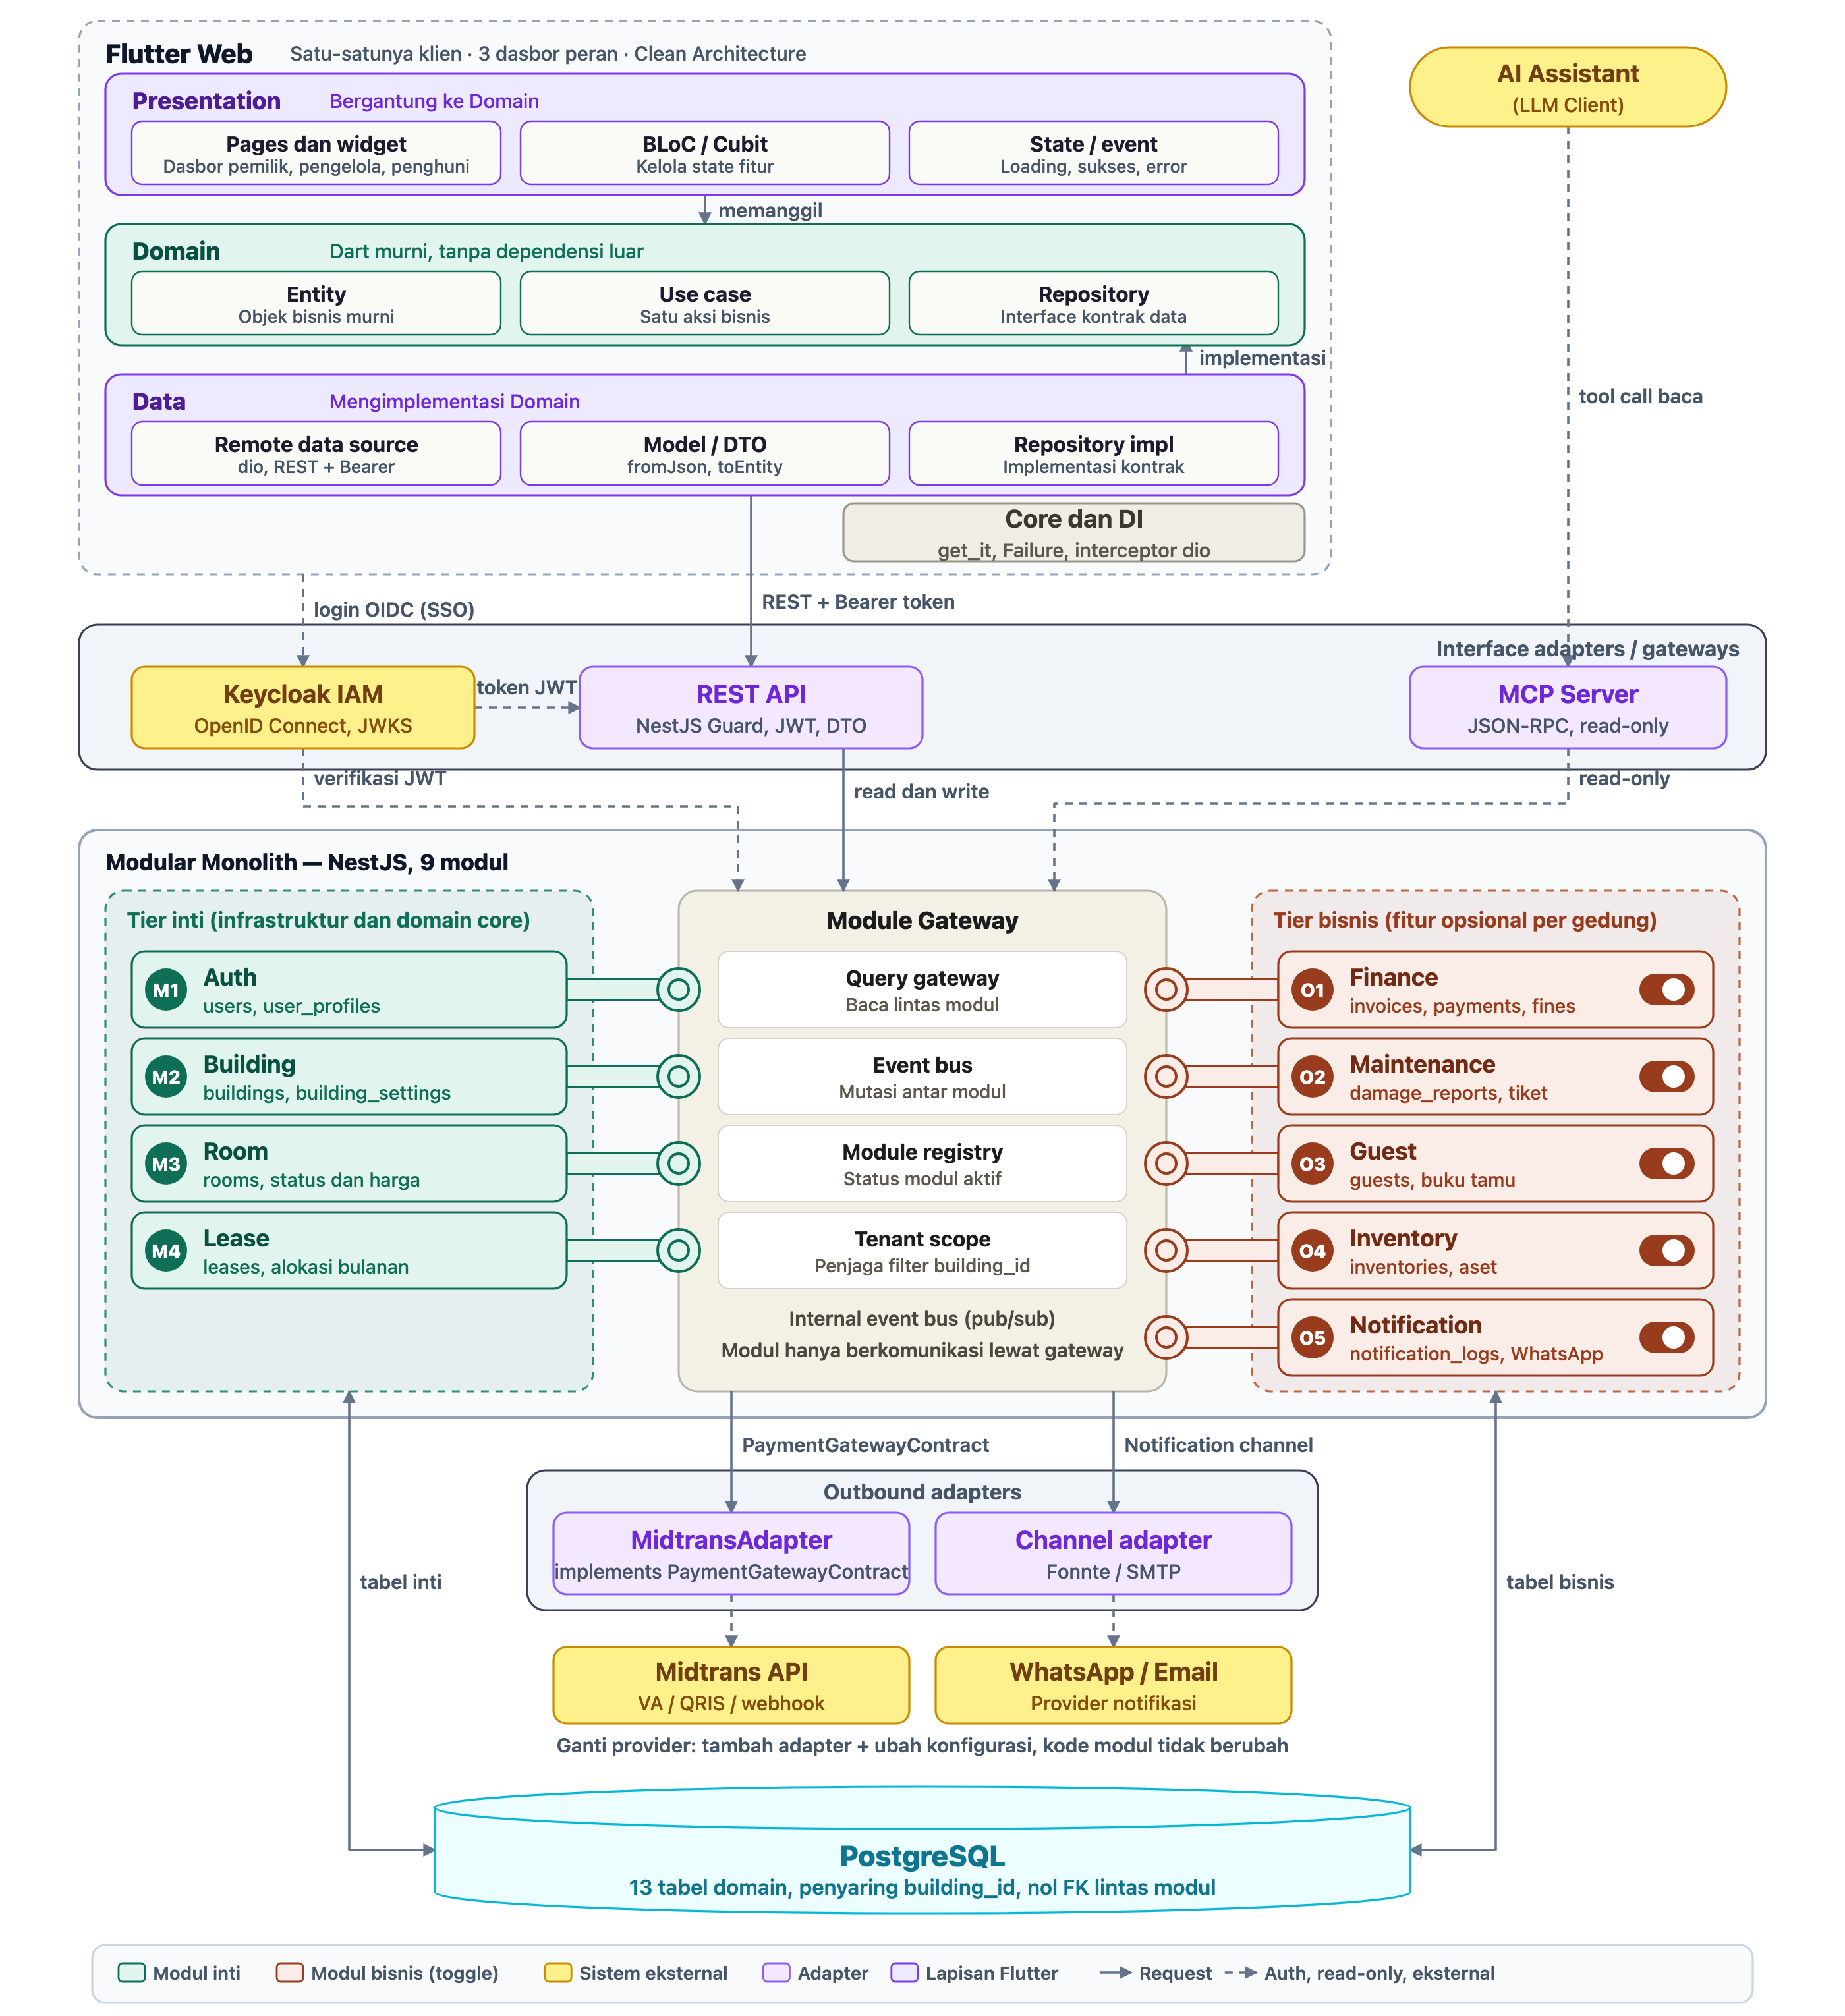
\includegraphics[width=0.95\textwidth,height=0.72\textheight,keepaspectratio]{assets/diagrams/bab3_01_arsitektur_terpadu.png}
  \caption{Arsitektur Sistem Keseluruhan}
  \label{fig:arsitektur_terpadu}
\end{figure}

Berdasarkan Gambar~\ref{fig:arsitektur_terpadu}, sistem terbagi menjadi empat lapisan utama:
\begin{enumerate}[label=\arabic*., leftmargin=*]
  \item \textbf{Lapisan Antarmuka (Flutter Web).} Lapisan ini menyajikan antarmuka pengguna berbasis peramban (\textit{web browser}) untuk tiga peran: Dasbor Pemilik untuk melihat ringkasan portofolio lintas gedung, Dasbor Pengelola untuk operasional harian satu gedung binaan, dan Portal Penghuni untuk memilih kamar, membayar tagihan, serta menyampaikan keluhan. Pada dasbor pemilik dan pengelola juga tersedia Tab Asisten AI untuk mengajukan pertanyaan analitik operasional.
  \item \textbf{Lapisan Adapter, Identitas, dan Protokol AI.} Lapisan ini menjembatani lalu lintas data dari luar menuju modul internal:
    \begin{enumerate}[label=\alph*., leftmargin=*]
      \item \textbf{Keycloak OIDC:} Menangani autentikasi identitas terpusat dan menerbitkan token akses JWT. Backend NestJS memverifikasi keabsahan token tersebut secara \textit{stateless} menggunakan kunci publik JWKS tanpa perlu menghubungi server Keycloak pada setiap permintaan.
      \item \textbf{REST API NestJS:} Menyediakan antarmuka komunikasi data HTTP yang terstandarisasi dengan amplop JSON seragam, validasi ketat DTO (\textit{Data Transfer Object}), dan dokumentasi interaktif Swagger.
      \item \textbf{MCP Server \& Klien MCP:} Menjalankan protokol \textit{Model Context Protocol} (MCP) berbasis format JSON-RPC 2.0. Klien AI (model bahasa besar/LLM) mengirimkan permintaan pemanggilan alat (\textit{tool call}), lalu Modul \texttt{AI / MCP Assistant} mengeksekusi kueri agregasi baca secara terukur melalui \textit{Module Gateway} dan mengembalikan data faktual operasional.
    \end{enumerate}
  \item \textbf{Lapisan Backend Modular Monolith.} Inti pemrosesan sistem dibangun dengan kerangka kerja NestJS yang membagi fungsi bisnis ke dalam sepuluh modul terenkapsulasi (4 modul \textit{core} dan 6 modul \textit{opsional}). Antar-modul berkomunikasi melalui \textit{event bus} untuk aksi mutasi data dan melalui \textit{query gateway} untuk pembacaan lintas domain, tanpa relasi fisik antar-tabel. Di bagian luar, backend terhubung ke penyedia gerbang pembayaran Midtrans melalui \texttt{MidtransAdapter} dan ke penyedia WhatsApp Gateway melalui \texttt{WhatsAppAdapter}.
  \item \textbf{Lapisan Data (PostgreSQL).} Berupa basis data relasional tunggal (\textit{shared database}). Seluruh data operasional diisolasi per gedung menggunakan \textit{row-level scoping} berbasis kolom \texttt{building\_id}.
\end{enumerate}

\subsection{Klasifikasi Modul: Core dan Opsional}

Sistem dibangun dengan arsitektur Modular Monolith menggunakan NestJS. Setiap modul terenkapsulasi dan tidak saling terikat melalui Foreign Key fisik lintas modul. Komunikasi antar modul dilakukan melalui \textit{event bus} untuk aksi mutasi dan \textit{module gateway} untuk pembacaan lintas domain. Pembagian sepuluh modul dirangkum pada Tabel~\ref{tab:klasifikasi_modul}.

\begin{longtblr}[
  caption = {Klasifikasi Modul Core dan Opsional},
  label = {tab:klasifikasi_modul}
]{
  width = \textwidth,
  colspec = {X[1.1,l] X[1.2,l] X[1.1,l] X[1.6,l] X[2.0,l]}
}
  Klasifikasi & Modul (Istilah Teknis) & Nama Fungsi Awam & Tabel Utama & Karakteristik \\
  \textbf{Core (Wajib Aktif)} & User \& Access Control & Pengguna \& Akses & \texttt{users}, \texttt{user\_profiles}, \texttt{roles}, \texttt{permissions}, \texttt{role\_permissions} & Konteks identitas dan peran pengguna. Harus selalu aktif. \\
  & Property \& Building & Gedung & \texttt{buildings}, \texttt{building\_settings} & Master gedung dan konfigurasi kebijakan per gedung. \\
  & Room Management & Kamar & \texttt{rooms} & Data fisik unit kamar. \\
  & Occupancy \& Schedule & Sewa \& Penempatan & \texttt{occupancies}, \texttt{occupancy\_members} & Kontrak sewa dan alokasi hunian (disertai tampilan \textit{Occupancy Dashboard}). \\
  \textbf{Opsional (Plug \& Play)} & Finance \& Billing & Keuangan \& Tagihan & \texttt{invoices}, \texttt{payments}, \texttt{fines}, \texttt{expenses} & Aktif untuk properti berbayar; bisa dinonaktifkan pada asrama/mes gratis. \\
  & Maintenance \& Facility & Perawatan & \texttt{damage\_reports}, \texttt{maintenance\_schedules} & Aktif jika gedung butuh tiket kerusakan dan jadwal perawatan. \\
  & Asset \& Inventory & Inventaris & \texttt{inventories}, \texttt{room\_inventories} & Aktif jika gedung memiliki inventaris perabot. \\
  & Guest Logging & Buku Tamu & \texttt{guests} & Aktif jika properti mencatat tamu. \\
  & Notification Service & Notifikasi & \texttt{notification\_logs} & Aktif jika terhubung ke gateway pesan. \\
  & AI / MCP Assistant & Asisten Analitik AI & --- (\textit{stateless read-only} via Gateway) & Modul AI yang membaca agregasi data lintas modul secara aman dan terisolasi per gedung. \\
\end{longtblr}

\textbf{Aturan utama:} Empat modul inti (\textit{core}) wajib aktif di semua kombinasi skenario. Enam modul tambahan (\textit{opsional}, termasuk Modul \texttt{AI / MCP Assistant}) dapat diaktifkan atau dinonaktifkan per gedung tanpa memutus modul lain.

Untuk memudahkan pemahaman bagi orang awam maupun penguji, konsep modularitas ini diilustrasikan dengan analogi susunan balok Lego pada Gambar~\ref{fig:klasifikasi_modul}.

\begin{figure}[H]
  \centering
  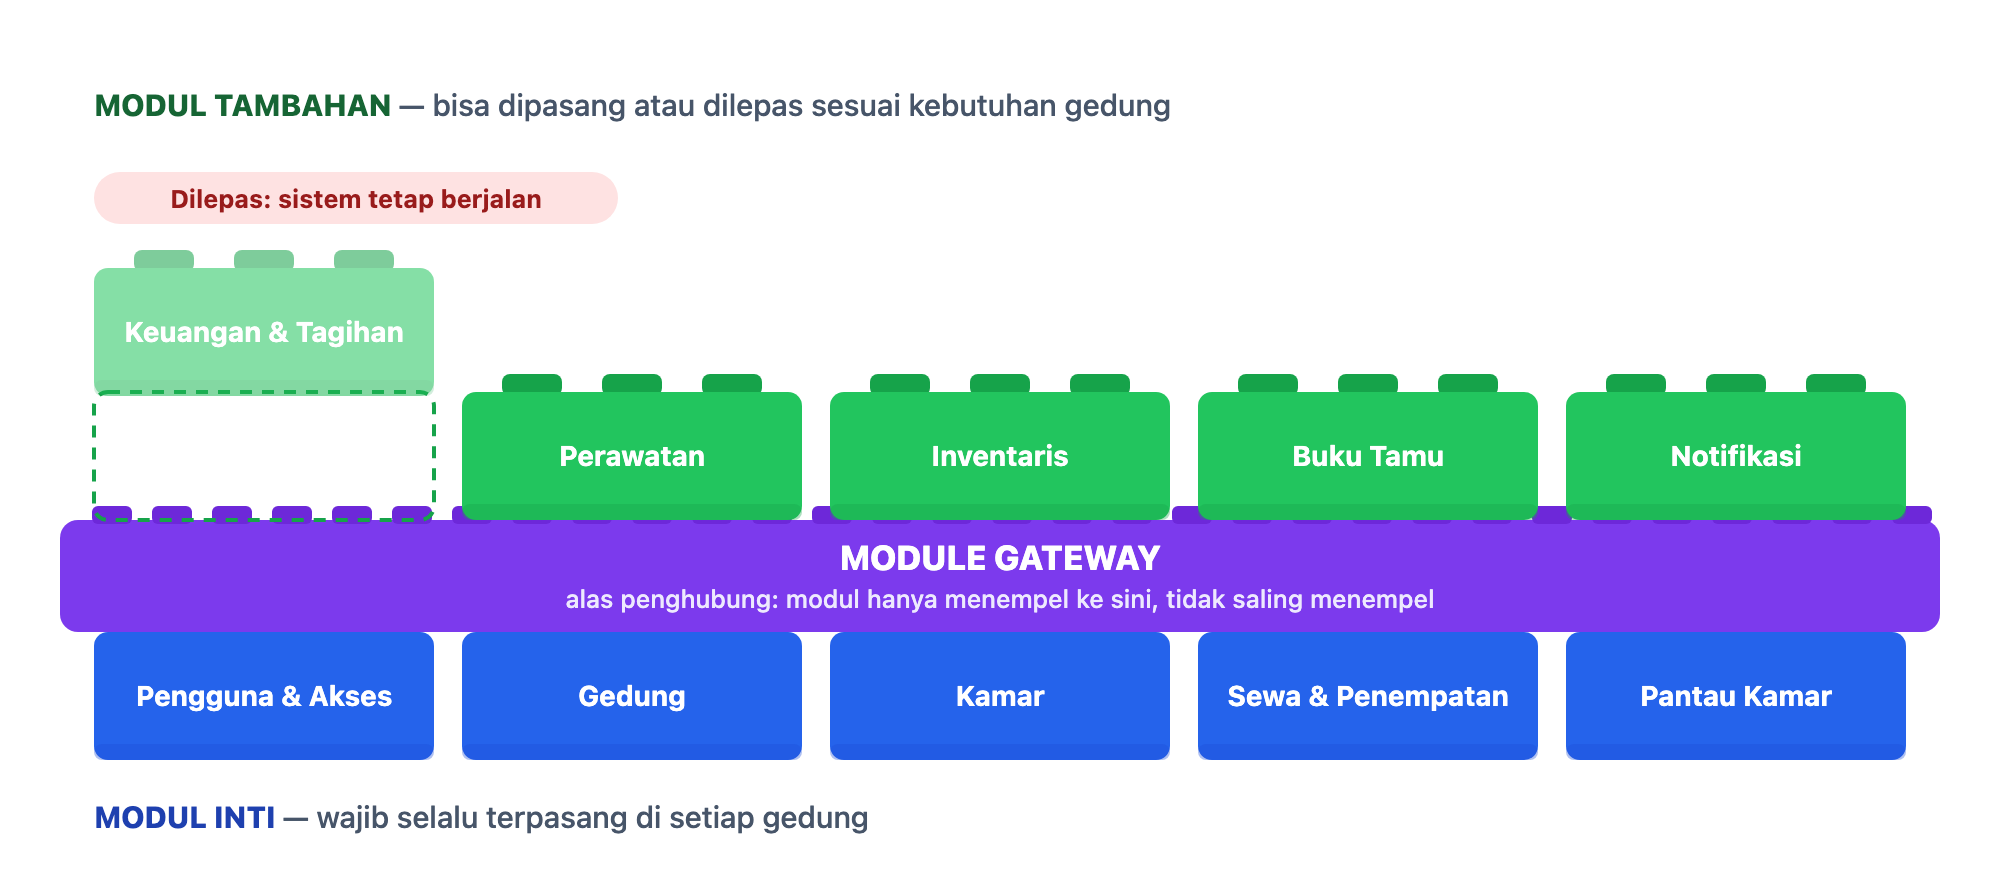
\includegraphics[width=0.95\textwidth,height=0.68\textheight,keepaspectratio]{assets/diagrams/bab3_02_klasifikasi_modul_lego.png}
  \caption{Arsitektur Modular Monolith}
  \label{fig:klasifikasi_modul}
\end{figure}

Berdasarkan Gambar~\ref{fig:klasifikasi_modul}, cara kerja modularitas sistem dapat dianalogikan sebagai berikut:
\begin{enumerate}[label=\arabic*., leftmargin=*]
  \item \textbf{Module Gateway sebagai Papan Alas (\textit{Baseplate} ungu):} Bertindak sebagai penghubung komunikasi pusat. Semua modul hanya menancap pada alas ini dan tidak saling mengikat secara langsung antar-balok.
  \item \textbf{Modul Inti sebagai Balok Pondasi (Balok biru di bawah):} Modul-modul inti terpasang permanen pada papan alas. Tanpa balok inti ini, struktur sistem tidak dapat berdiri.
  \item \textbf{Modul Tambahan sebagai Balok Bongkar-Pasang (Balok hijau di atas):} Modul-modul bisnis dan asisten analitik dapat dipasang (\textit{ON}) atau dicabut (\textit{OFF}) secara fleksibel sesuai profil operasional masing-masing gedung.
  \item \textbf{Independensi saat Modul Dilepas:} Balok \textit{Keuangan \& Tagihan} digambarkan terangkat dari posisinya untuk mencontohkan kondisi asrama mahasiswa atau mes karyawan gratis yang tidak memungut biaya sewa. Ketika balok keuangan dilepas, papan alas dan balok lainnya tetap kokoh berdiri tanpa memicu kesalahan (\textit{crash} atau galat basis data).
\end{enumerate}

\subsubsection{Konteks Data Antar-Modul (Tanpa FK Fisik)}

Seluruh modul berbagi satu basis data PostgreSQL dengan isolasi baris (\textit{row-level scoping}) melalui kolom \texttt{building\_id}. Modul yang membutuhkan konteks gedung atau pengguna \textbf{tidak mengakses tabel modul lain secara langsung}, melainkan memperolehnya dari klaim token akses JWT yang divalidasi oleh backend:
\begin{enumerate}[label=\arabic*., leftmargin=*]
  \item Modul Keuangan mengetahui \texttt{building\_id} dari klaim token, bukan dengan \textit{join} langsung ke tabel \texttt{buildings}.
  \item Modul Kamar menerima \texttt{building\_id} dari parameter permintaan yang telah divalidasi terhadap klaim token, bukan melalui relasi FK fisik ke tabel \texttt{buildings}.
\end{enumerate}

Dengan pola ini, menonaktifkan satu modul opsional tidak memicu kesalahan integritas data pada modul lain.

\subsection{Arsitektur Backend}

Berbeda dengan arsitektur sebelum \textit{rewrite} pada Gambar~\ref{fig:arsitektur_lama} yang mengizinkan pemanggilan langsung antar-\textit{service} lintas domain, pada rancangan baru ini \textit{backend} NestJS dipecah ke dalam sepuluh modul yang dikelompokkan ke dalam tiga tingkatan (\textit{tier}) logis, sebagaimana ditunjukkan pada Gambar~\ref{fig:arsitektur_backend}. Pengelompokan ini bertujuan menjaga keteraturan arah ketergantungan agar modul tingkat dasar tidak bergantung pada modul tingkat bisnis, serta mewajibkan seluruh komunikasi lintas modul melewati \textit{Module Gateway}.

\begin{figure}[H]
  \centering
  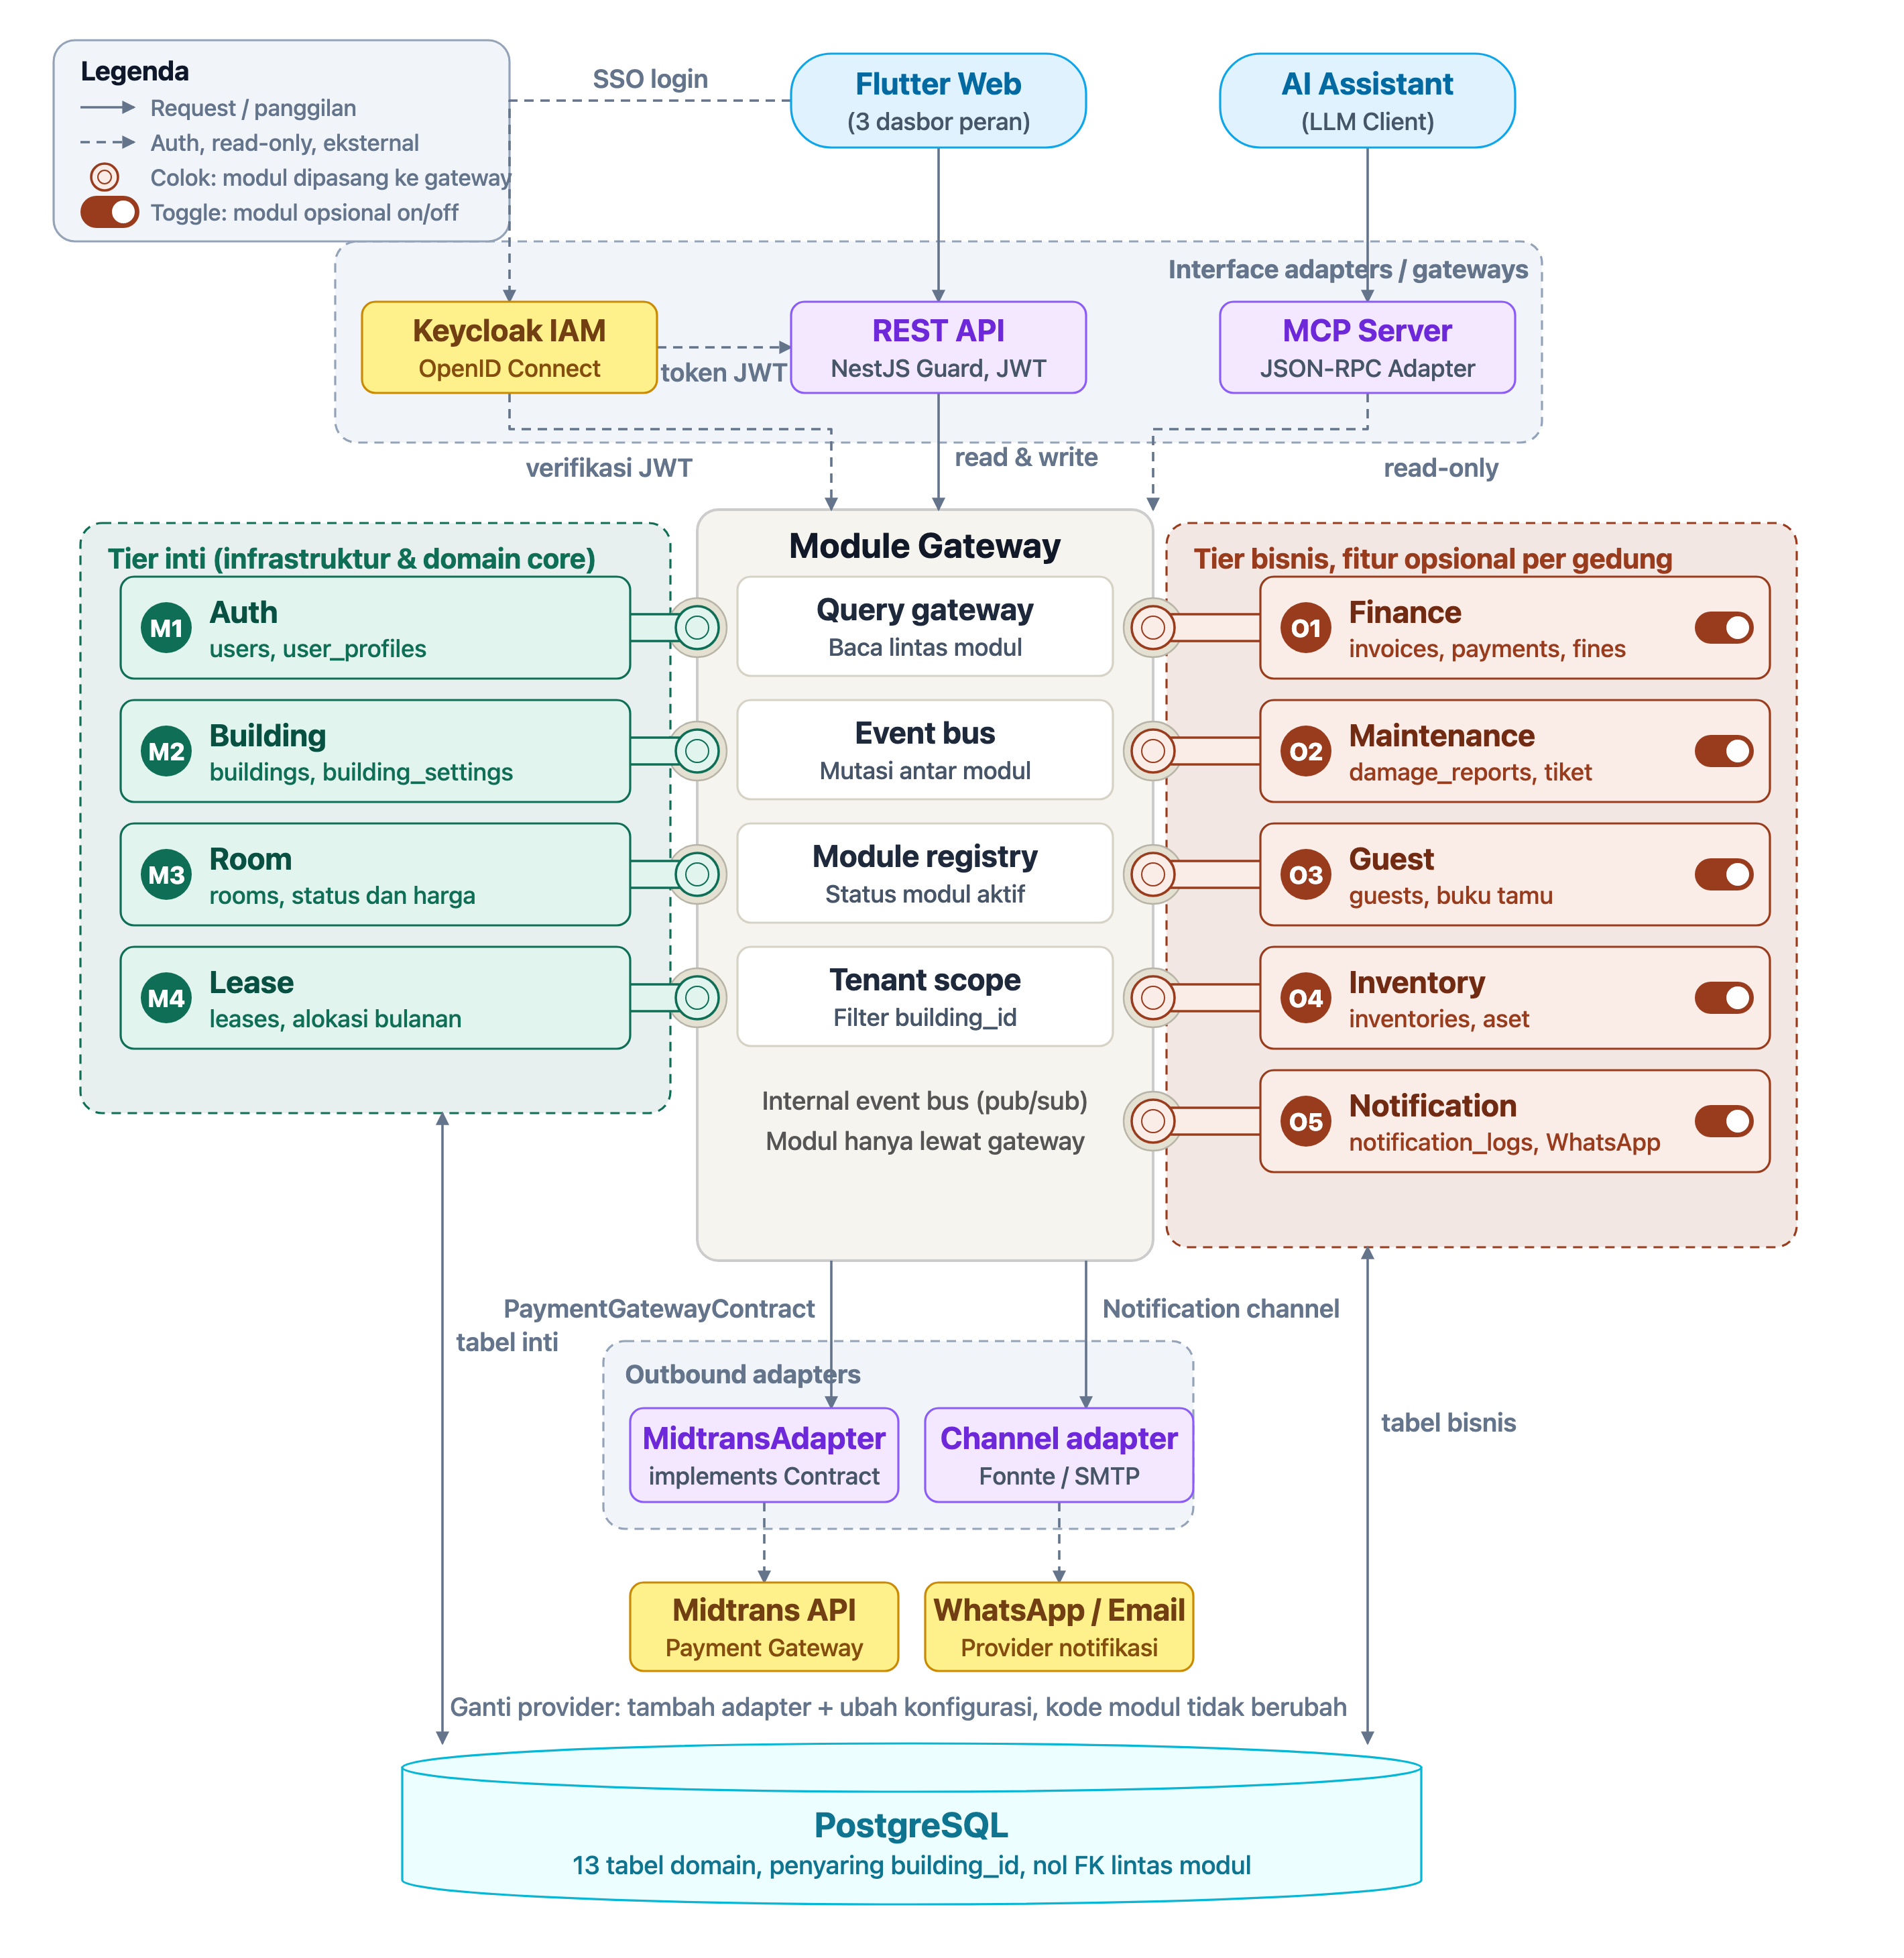
\includegraphics[width=0.95\textwidth,height=0.72\textheight,keepaspectratio]{assets/diagrams/bab3_03_arsitektur_backend.png}
  \caption{Dekomposisi Modul Backend NestJS}
  \label{fig:arsitektur_backend}
\end{figure}

Struktur tiga tingkatan modul backend tersebut meliputi:
\begin{enumerate}[label=\arabic*., leftmargin=*]
  \item \textbf{Tier 1 --- Modul Inti (\textit{Core Modules}).} Modul-modul ini wajib aktif di semua skenario implementasi karena menopang operasional dasar:
    \begin{enumerate}[label=\alph*., leftmargin=*]
      \item \textbf{M1 (Auth):} Mengelola otorisasi pengguna, pemetaan peran Keycloak (\texttt{owner}, \texttt{admin}, \texttt{resident}), dan profil biodata pada tabel \texttt{users} serta \texttt{user\_profiles}.
      \item \textbf{M2 (Building):} Mengelola master data gedung properti pada tabel \texttt{buildings}, serta aturan kebijakan huni pada tabel \texttt{building\_settings}.
      \item \textbf{M3 (Room):} Mengelola data fisik unit kamar, nomor, tipe, tarif sewa, dan status kesiapan unit (\texttt{kosong}, \texttt{terisi}, \texttt{maintenance}) pada tabel \texttt{rooms}.
      \item \textbf{M4 (Lease / Occupancy):} Mengelola siklus kontrak sewa bulanan dan penempatan kamar pada tabel \texttt{occupancies}, dilengkapi penguncian baris (\textit{row locking}) untuk mencegah bentrok jadwal sewa.
    \end{enumerate}
  \item \textbf{Tier 2 --- Modul Bisnis \& Layanan Opsional (\textit{Optional Modules}).} Modul penunjang yang dapat diaktifkan atau dinonaktifkan sesuai kebutuhan masing-masing gedung:
    \begin{enumerate}[label=\alph*., leftmargin=*]
      \item \textbf{O1 (Finance):} Mengelola siklus penagihan berkala pada tabel \texttt{invoices}, pencatatan pembayaran digital Midtrans pada tabel \texttt{payments}, serta denda keterlambatan flat pada tabel \texttt{fines}.
      \item \textbf{O2 (Maintenance):} Mengelola penerimaan dan tindak lanjut laporan kerusakan fasilitas dari penghuni pada tabel \texttt{damage\_reports}.
      \item \textbf{O3 (Inventory):} Mengelola inventaris aset perabot kamar dan kondisinya pada tabel \texttt{inventories} serta \texttt{room\_inventories}.
      \item \textbf{O4 (Guest):} Mengelola pencatatan tamu yang berkunjung atau menginap pada tabel \texttt{guests}.
      \item \textbf{O5 (Notification):} Mengelola pencatatan riwayat pesan pengingat tagihan dan informasi operasional yang dikirim ke nomor WhatsApp penghuni pada tabel \texttt{notification\_logs}.
      \item \textbf{O6 (AI / MCP Assistant):} Modul kecerdasan buatan berbasis \textit{Model Context Protocol} yang menyediakan perkakas baca (\textit{read-only tools}) terstandarisasi bagi LLM untuk menjawab pertanyaan manajerial pemilik/pengelola melalui \textit{Query Gateway} tanpa akses tulis langsung ke basis data.
    \end{enumerate}
  \item \textbf{Tier 3 --- Module Gateway dan Layanan Bersama.}
    \begin{enumerate}[label=\alph*., leftmargin=*]
      \item \textbf{Query Gateway:} Menyediakan fungsi agregasi baca lintas modul sehingga satu modul (termasuk Modul \texttt{AI / MCP Assistant}) tidak perlu melakukan kueri langsung ke tabel milik modul lain.
      \item \textbf{Event Bus:} Menyediakan jalur pengiriman pesan kejadian asinkron (\textit{domain events}). Sebagai contoh, saat kontrak sewa baru terbentuk di modul Lease, event \texttt{LeaseCreated} dikirimkan ke modul Finance untuk menerbitkan invoice pertama dan ke modul Notification untuk mengirimkan pemberitahuan.
      \item \textbf{Module Registry:} Memeriksa status fitur modul per gedung berdasarkan konfigurasi \texttt{building\_settings}.
      \item \textbf{Tenant Scope:} Memastikan setiap kueri basis data menyertakan klaim \texttt{building\_id} milik pengguna yang aktif.
    \end{enumerate}
\end{enumerate}

\subsection{Arsitektur Antarmuka Pengguna (Clean Architecture pada Flutter Web)}

Antarmuka web dikembangkan menggunakan Flutter Web dengan menerapkan pola \textit{Clean Architecture}. Kode aplikasi dipisahkan secara tegas antara komponen tampilan dan aturan logika bisnis, sehingga antarmuka mudah dirawat dan siap diuji secara mandiri.

\begin{figure}[H]
  \centering
  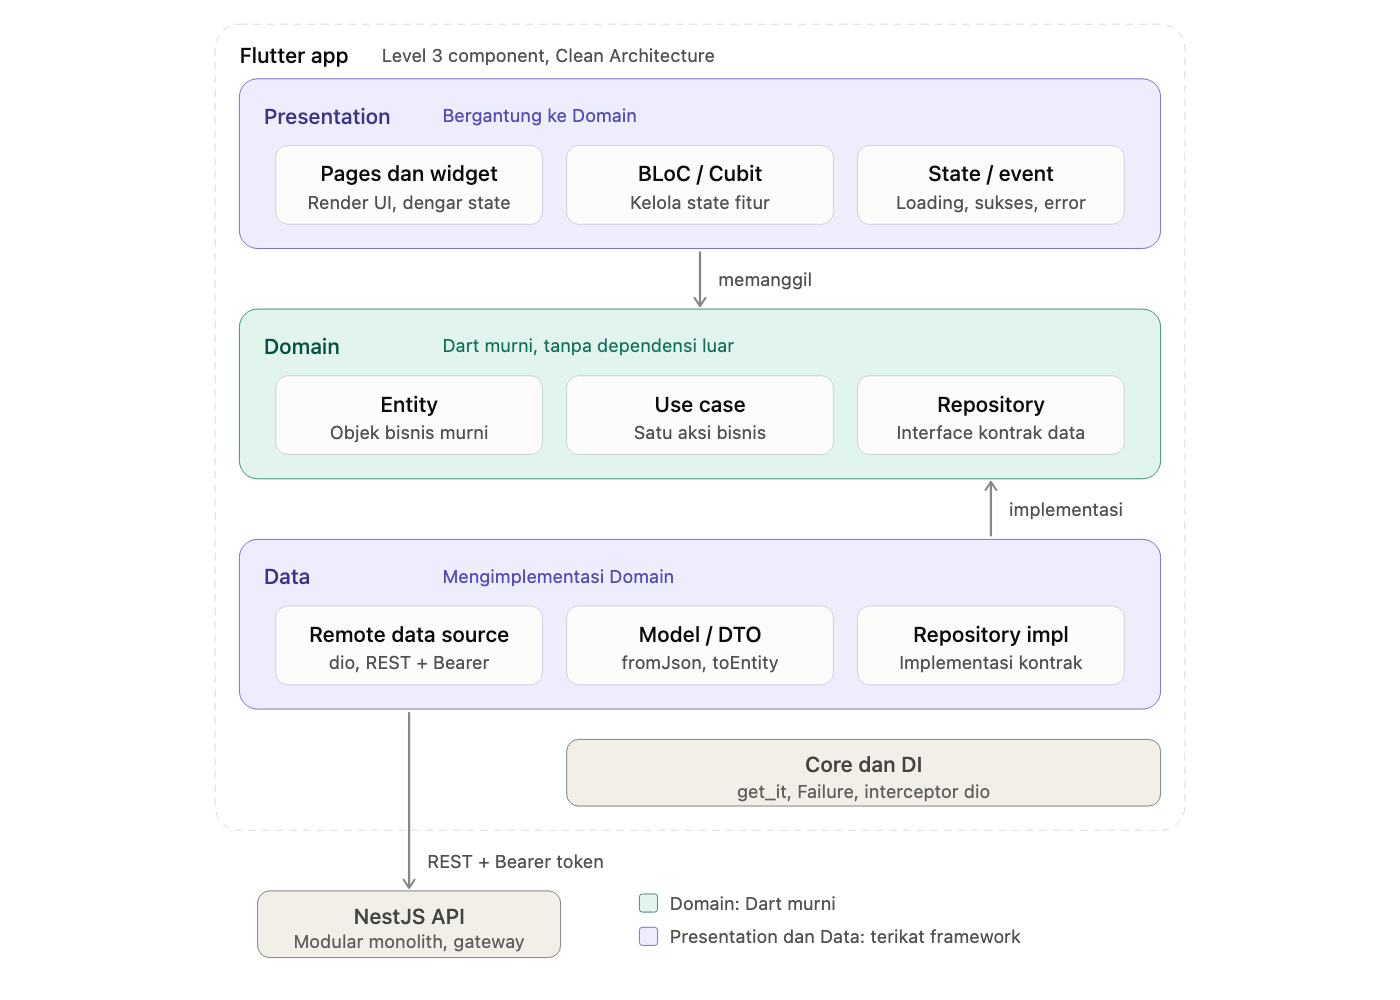
\includegraphics[width=0.84\textwidth,height=0.68\textheight,keepaspectratio]{assets/diagrams/bab3_04_arsitektur_frontend.png}
  \caption{Arsitektur Antarmuka Flutter Web berbasis Clean Architecture}
  \label{fig:arsitektur_frontend}
\end{figure}

Gambar~\ref{fig:arsitektur_frontend} memperlihatkan tiga lapisan utama pada aplikasi Flutter Web beserta komponen penunjangnya:
\begin{enumerate}[label=\arabic*., leftmargin=*]
  \item \textbf{Lapisan Presentasi (\textit{Presentation Layer}).} Lapisan terluar yang berhubungan langsung dengan pengguna. Terdiri dari \textit{Pages and Widgets} yang bertugas merender tampilan visual halaman serta menangkap aksi masukan pengguna, dan komponen \textit{BLoC / Cubit} (\textit{Business Logic Component}) yang mengelola \textit{state} fitur. BLoC menerima masukan berupa \textit{event}, memprosesnya ke lapisan domain, lalu memancarkan status perubahan (\textit{loading}, \textit{sukses}, \textit{error}) ke antarmuka.
  \item \textbf{Lapisan Domain (\textit{Domain Layer}).} Inti dari aplikasi yang ditulis menggunakan bahasa Dart murni tanpa ketergantungan pada pustaka antarmuka Flutter maupun pustaka pihak ketiga. Lapisan ini memuat:
    \begin{enumerate}[label=\alph*., leftmargin=*]
      \item \textbf{Entity:} Objek representasi data bisnis murni (misalnya \texttt{Room}, \texttt{Lease}, \texttt{DamageReport}).
      \item \textbf{Use Case:} Komponen yang mengeksekusi satu aksi bisnis spesifik (seperti alokasi kamar sewa, pelaporan kerusakan, atau penarikan tagihan).
      \item \textbf{Repository (Interface):} Kontrak abstrak yang mendefinisikan kebutuhan operasi data tanpa terikat pada bagaimana data tersebut diambil.
    \end{enumerate}
  \item \textbf{Lapisan Data (\textit{Data Layer}).} Lapisan yang bertanggung jawab mengimplementasikan kontrak repositori yang didefinisikan oleh lapisan domain. Terdiri dari:
    \begin{enumerate}[label=\alph*., leftmargin=*]
      \item \textbf{Remote Data Source:} Bertugas melakukan panggilan jaringan HTTP ke backend NestJS menggunakan pustaka Dio dengan menyertakan \textit{Bearer token} JWT.
      \item \textbf{Model / DTO:} Menangani serialisasi dan deserialisasi JSON (\texttt{fromJson}) serta memetakan data respons API ke entitas domain (\texttt{toEntity}).
      \item \textbf{Repository Implementation:} Mengoordinasikan pengambilan data dari \textit{data source} dan mengubahnya menjadi format domain sebelum diteruskan ke \textit{use case}.
    \end{enumerate}
  \item \textbf{Lapisan Core dan Dependency Injection.} Fondasi teknis yang digunakan bersama di seluruh lapisan, meliputi penanganan galat terpusat (\textit{Failure} dan \textit{Exception}), \textit{interceptor} Dio untuk menyematkan token autentikasi secara otomatis pada setiap \textit{header} permintaan, serta pengaturan injeksi dependensi menggunakan \textit{service locator} \texttt{get\_it}.
\end{enumerate}

\section{ALUR PROSES BISNIS}
\label{sec:alur_proses}

Bagian ini memodelkan seluruh proses operasional utama sistem menggunakan diagram aktivitas lintas lajur (\textit{swimlane activity diagram}). Notasi ini dipilih agar urutan aktivitas dan pertukaran data antar-aktor, sistem kost (antarmuka Flutter Web, modul backend NestJS, dan \textit{event bus}), serta layanan eksternal (Midtrans, WhatsApp Gateway, Keycloak, dan LLM) dapat ditelusuri langkah demi langkah.

\subsection{Alur Alokasi dan Penempatan Hunian}

Alur ini mengatur proses pemilihan kamar oleh penghuni, validasi batas minimum sewa gedung, pencegahan pemesanan ganda melalui penguncian baris basis data, hingga penerbitan kontrak sewa, seperti ditunjukkan pada Gambar~\ref{fig:alur_alokasi}.

\begin{figure}[H]
  \centering
  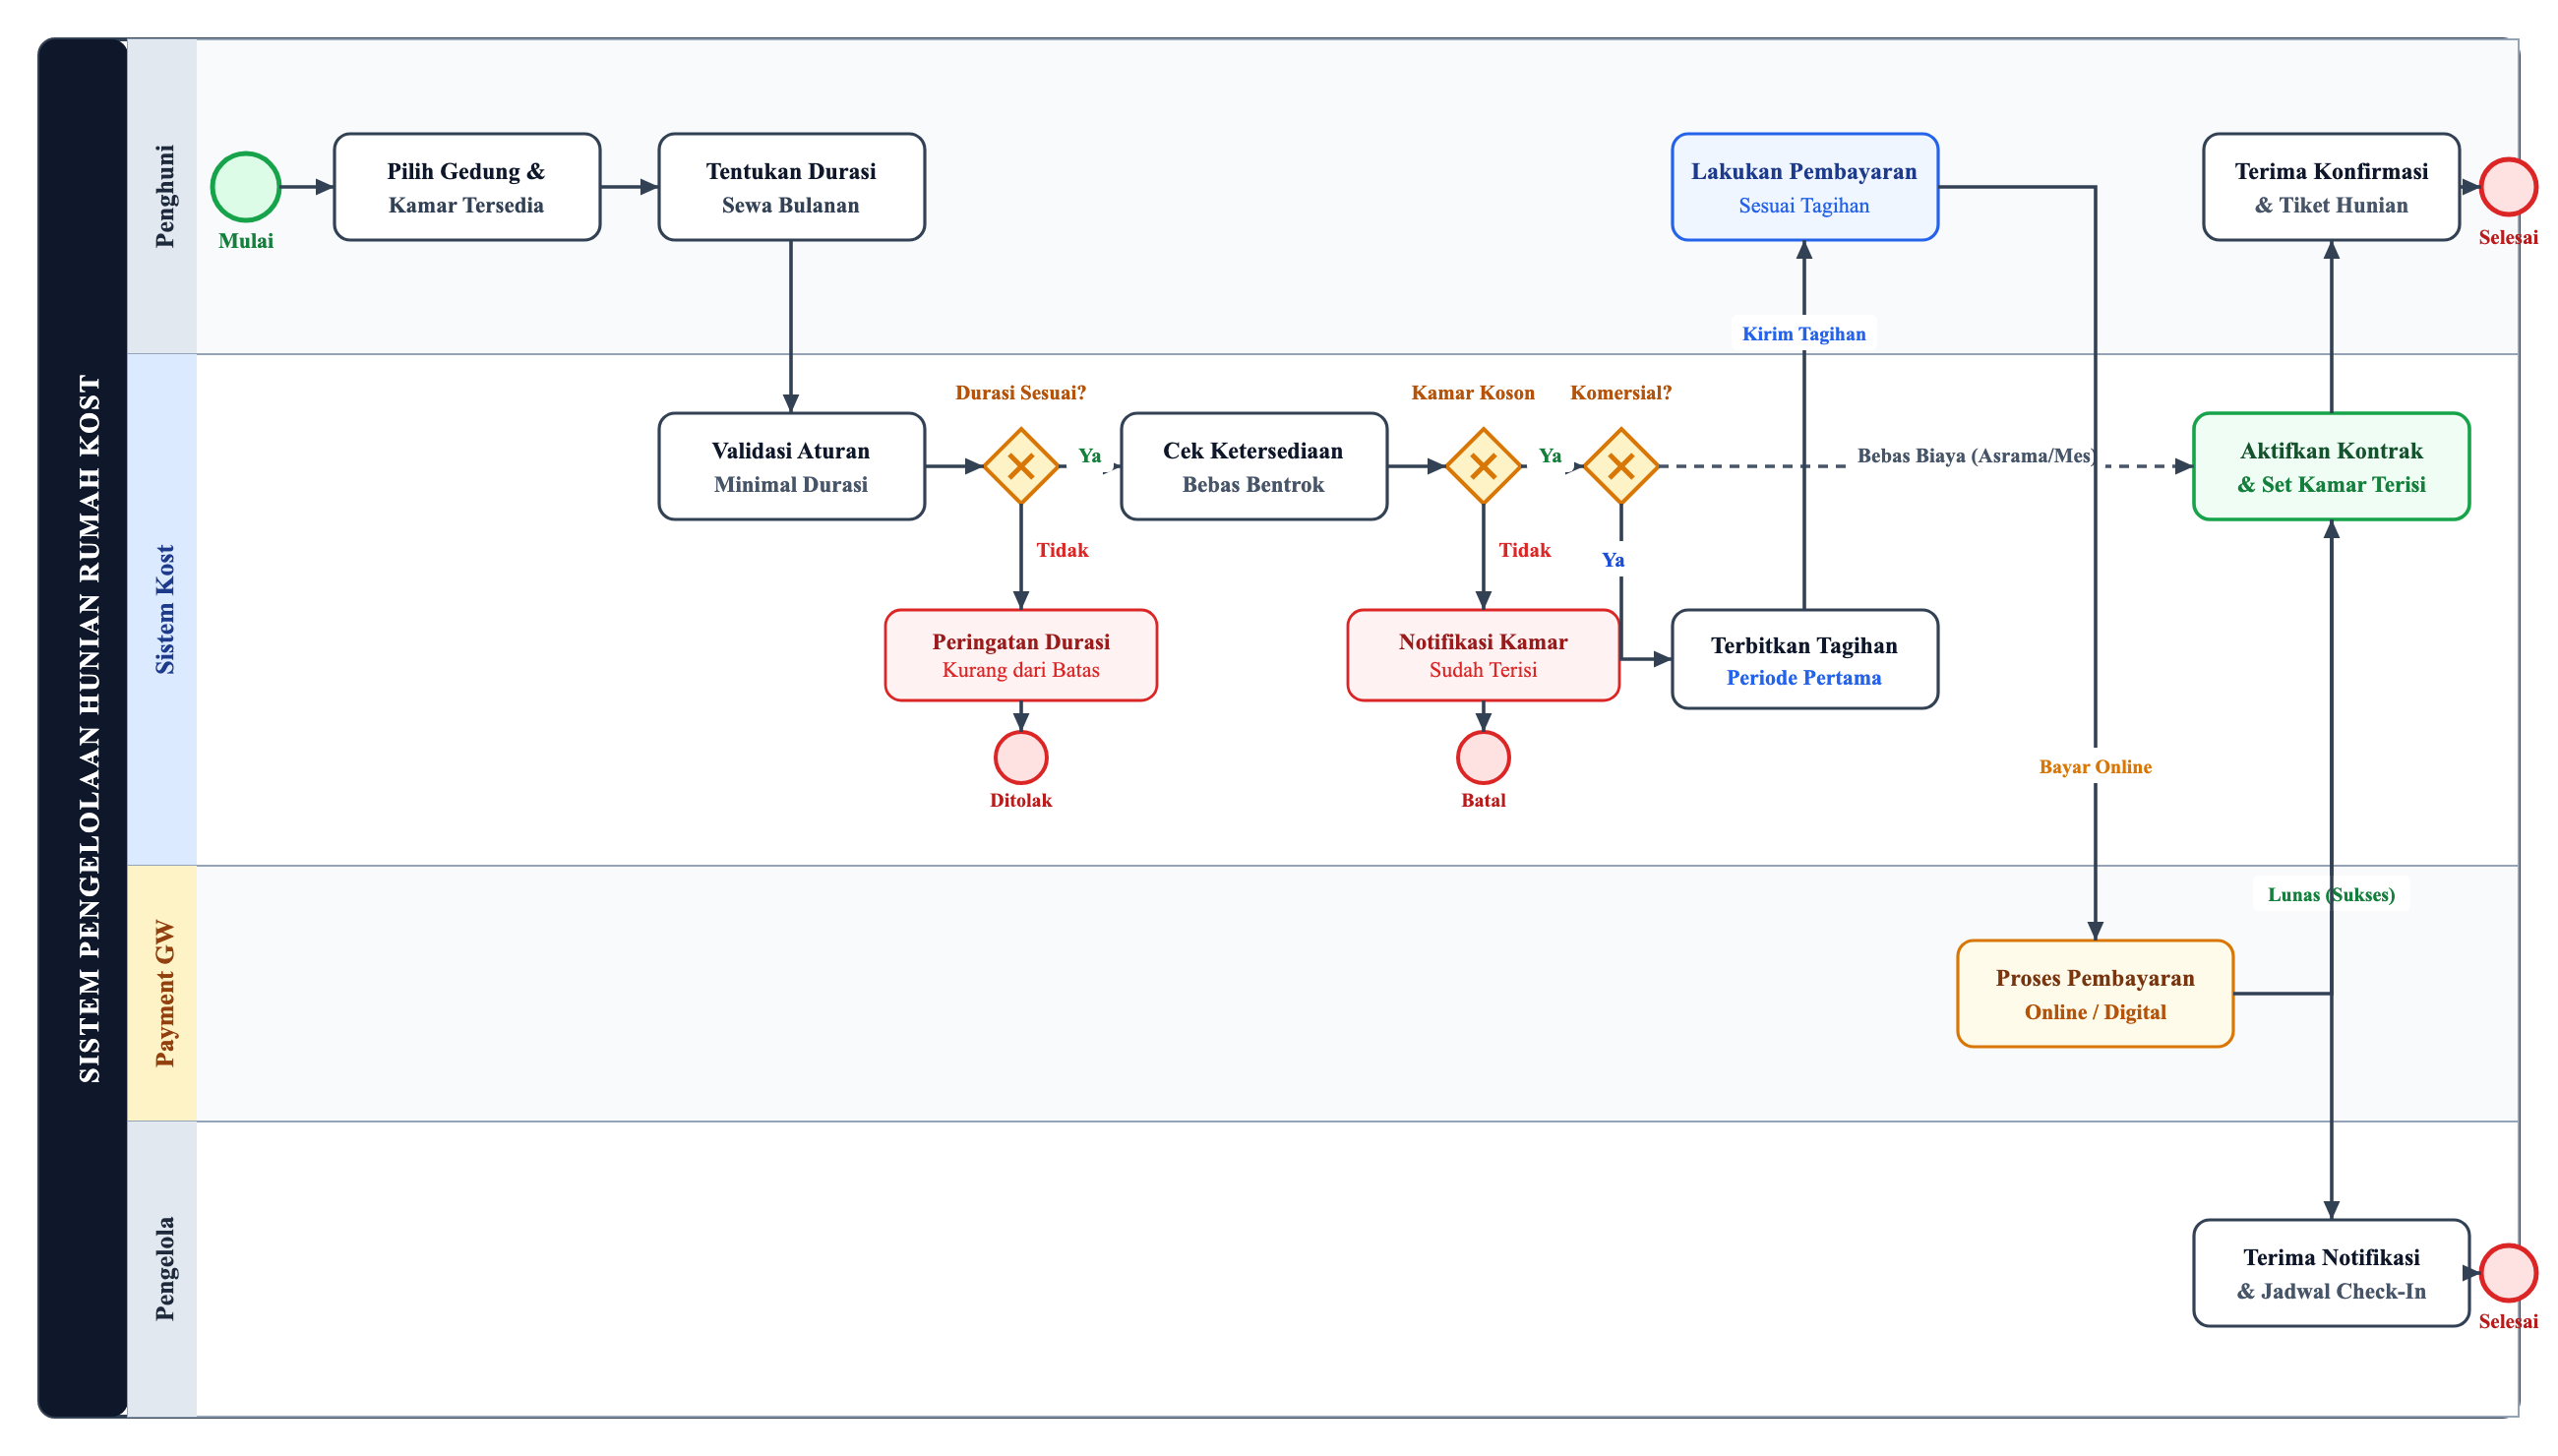
\includegraphics[width=0.96\textwidth,height=0.65\textheight,keepaspectratio]{assets/diagrams/bab3_05_alur_alokasi_penempatan.png}
  \caption{Diagram Alur Proses Alokasi dan Penempatan Hunian}
  \label{fig:alur_alokasi}
\end{figure}

Tahapan proses pada Gambar~\ref{fig:alur_alokasi} berjalan sebagai berikut:
\begin{enumerate}[label=\arabic*., leftmargin=*]
  \item Penghuni membuka katalog kamar pada antarmuka Flutter Web dengan memilih gedung yang dituju.
  \item Sistem memanggil modul Building dan modul Room menggunakan penyaring \texttt{building\_id} dari token sesi untuk menampilkan kamar berstatus kosong beserta tarif bulanannya.
  \item Penghuni memilih nomor unit kamar dan durasi sewa dalam satuan bulan, lalu menekan tombol pengajuan sewa.
  \item Modul Lease membaca konfigurasi \texttt{min\_rental\_months} pada tabel \texttt{building\_settings} via modul Building. Jika durasi yang diminta kurang dari batas minimum gedung, sistem langsung menolak dengan kode HTTP 422.
  \item Jika durasi memenuhi syarat, modul Lease membuka transaksi basis data dan mengunci baris kamar terkait menggunakan perintah \texttt{SELECT ... FOR UPDATE} guna memeriksa apakah ada kontrak aktif yang tumpang tindih. Jika kamar sedang diproses transaksi lain, sistem mengembalikan galat HTTP 422.
  \item Jika kamar kosong dan valid, modul Lease menyimpan data kontrak dengan status awal \texttt{pending\_payment} dan menerbitkan kejadian \texttt{LeaseCreated} ke \textit{event bus}.
  \item Pada properti komersial (modul Finance aktif), modul Finance menangkap kejadian tersebut, menerbitkan invoice periode pertama, meminta token transaksi SNAP ke Midtrans, dan mengembalikannya ke antarmuka untuk dibayar. Setelah notifikasi pelunasan diterima dari Midtrans via webhook, modul Lease mengubah status kontrak menjadi \texttt{confirmed} dan status kamar menjadi terisi.
  \item Mekanisme penagihan menerapkan skema Dua Fase (\textit{Two-Phase Invoicing}): Fase 1 menerbitkan invoice DP/\textit{booking fee} (atau pembayaran sewa bulan/periode pertama) untuk mengonfirmasi reservasi, dan Fase 2 menerbitkan invoice pelunasan atau sewa berkala berikutnya sebelum tanggal jatuh tempo huni.
  \item Pada properti non-komersial seperti asrama (modul Finance nonaktif), kontrak langsung berstatus \texttt{confirmed} tanpa menunggu pembayaran.
\end{enumerate}

\subsection{Alur Penagihan Sewa dan Pembayaran Digital}

Alur ini mengatur penerbitan tagihan berkala, opsi pembayaran otomatis melalui gerbang pembayaran Midtrans maupun manual melalui pengelola, penanganan denda keterlambatan, serta pengiriman bukti bayar otomatis via WhatsApp (Gambar~\ref{fig:alur_penagihan}).

\begin{figure}[H]
  \centering
  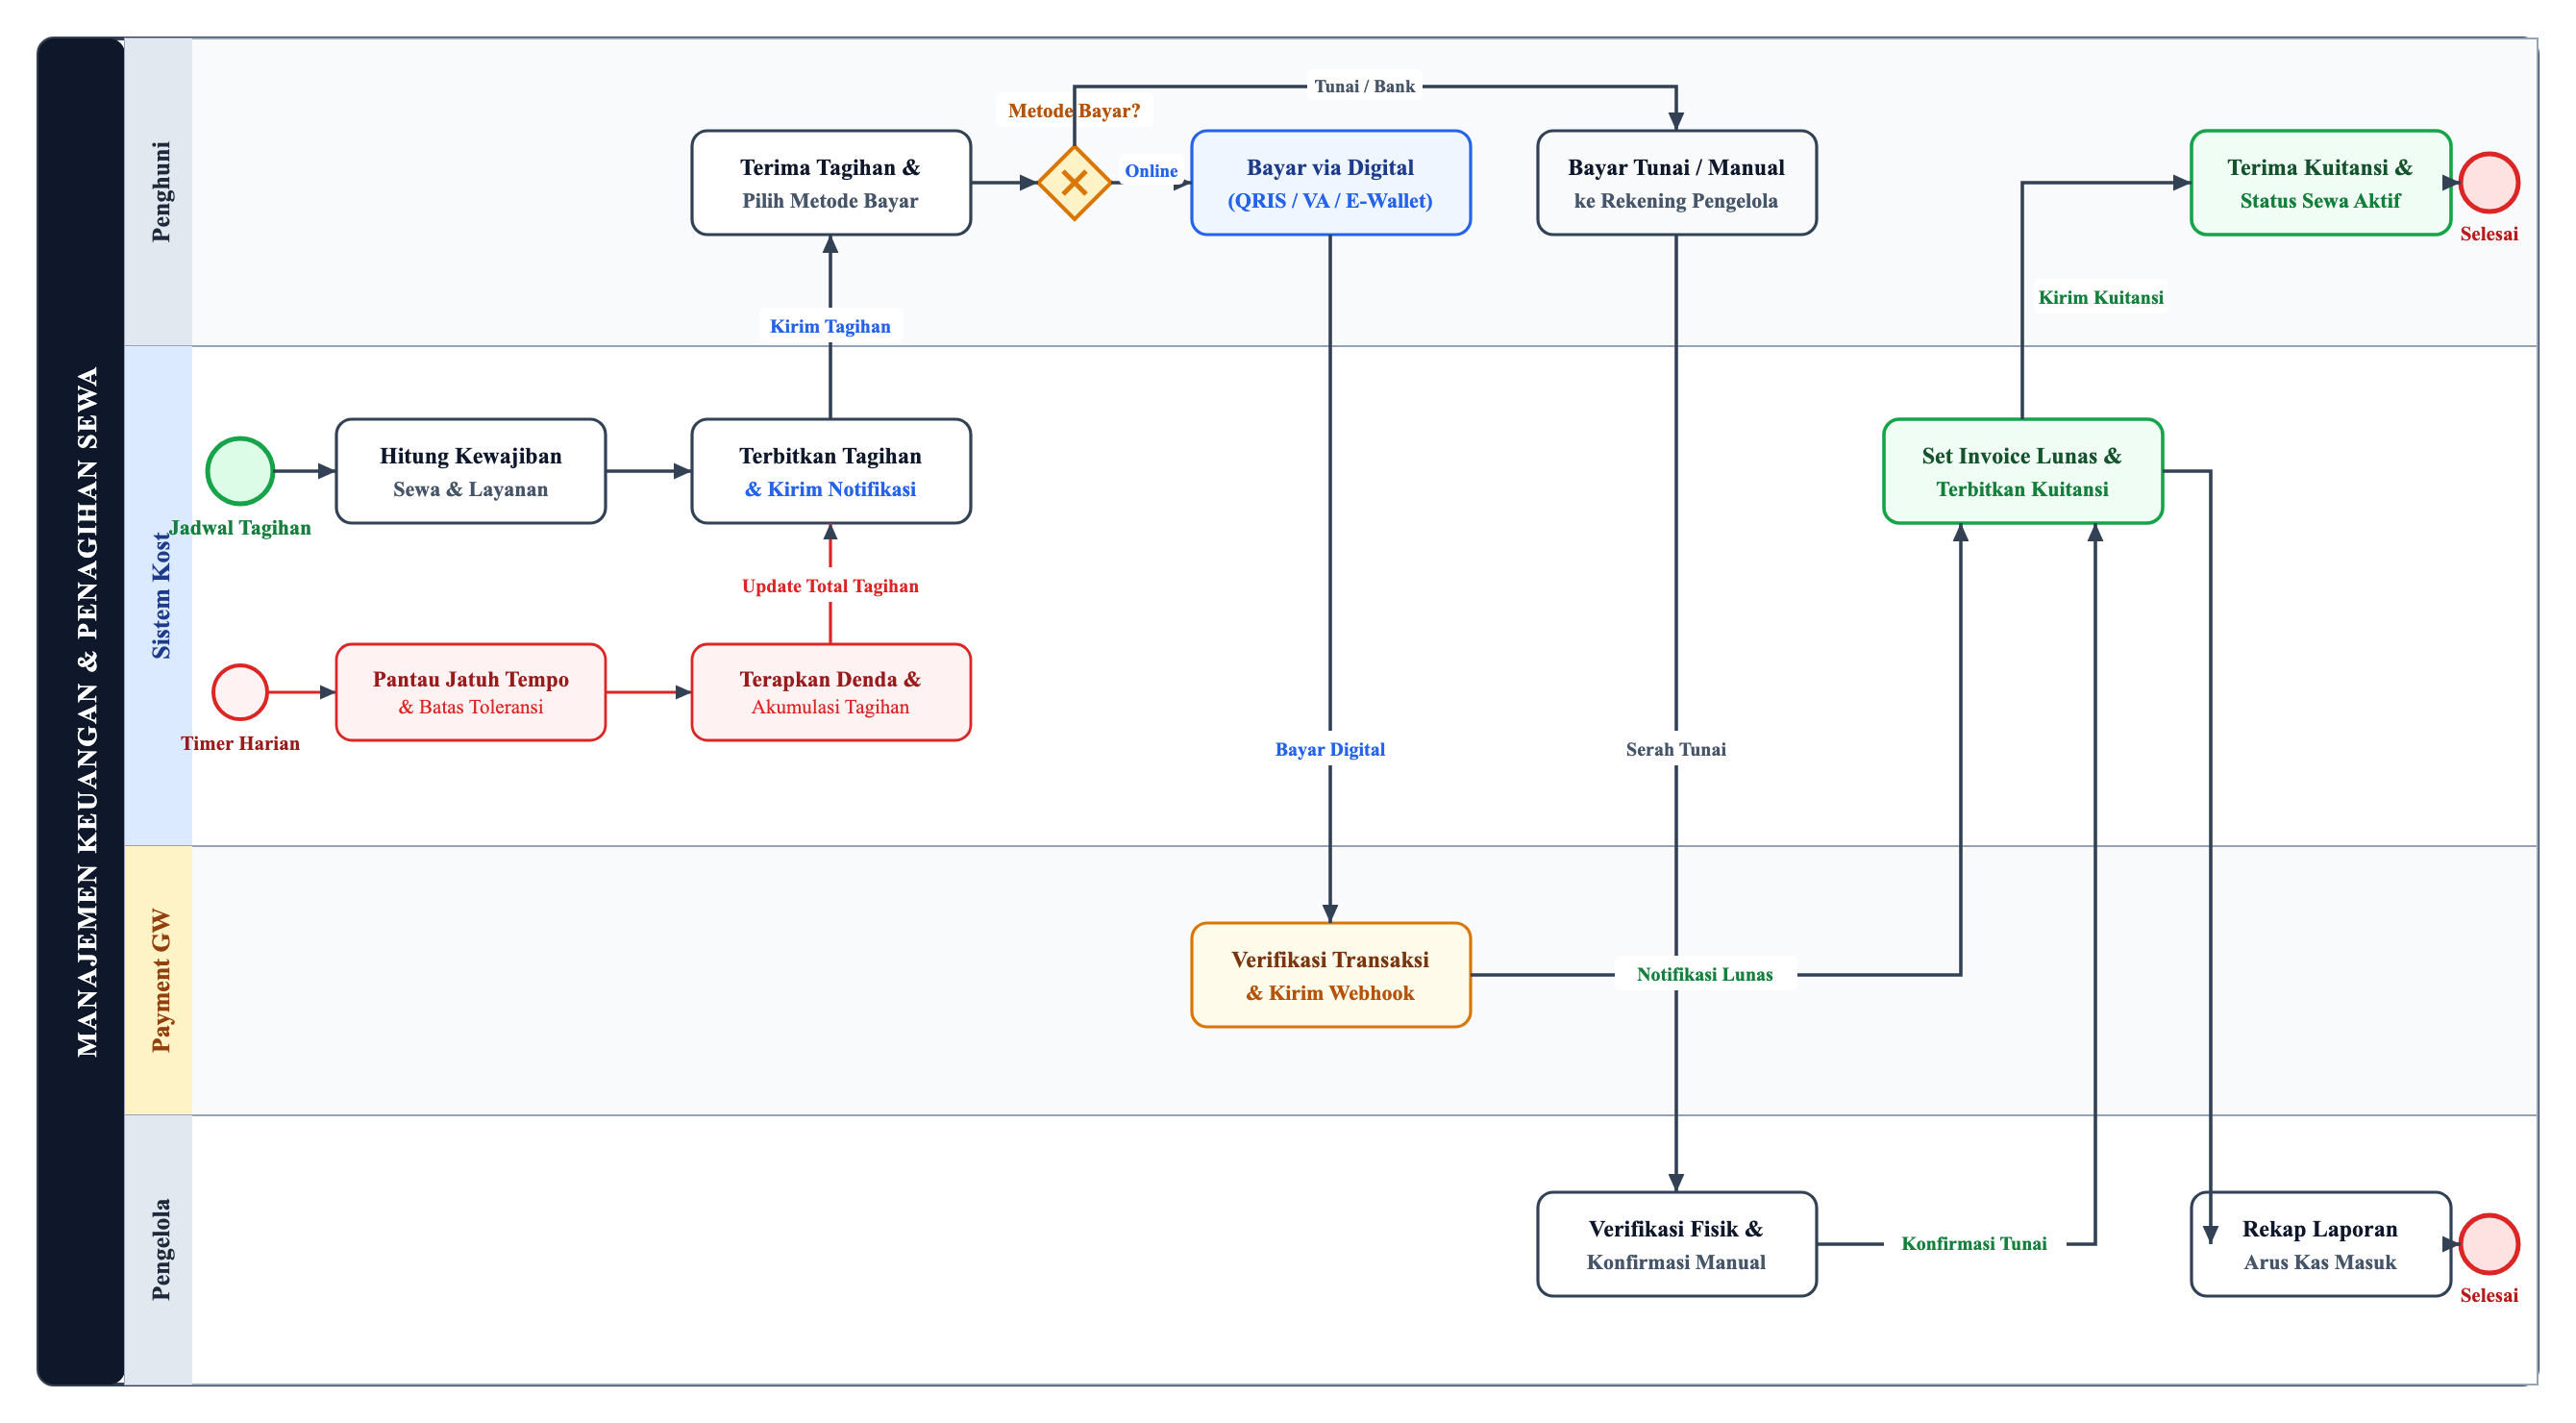
\includegraphics[width=0.96\textwidth,height=0.65\textheight,keepaspectratio]{assets/diagrams/bab3_06_alur_penagihan_pembayaran.png}
  \caption{Diagram Alur Proses Penagihan Sewa dan Pembayaran Digital}
  \label{fig:alur_penagihan}
\end{figure}

Tahapan proses pada Gambar~\ref{fig:alur_penagihan} meliputi:
\begin{enumerate}[label=\arabic*., leftmargin=*]
  \item Modul Finance menangkap kejadian \texttt{LeaseCreated} dari \textit{event bus}, menghitung total kewajiban sewa (harga bulanan dikalikan durasi periode berjalan), lalu menerbitkan invoice baru berstatus \texttt{unpaid} dengan tenggat jatuh tempo tertentu.
  \item Modul Finance menerbitkan event \texttt{InvoiceIssued}, yang ditangkap oleh modul Notification untuk mengirimkan tautan rincian tagihan ke nomor WhatsApp penghuni.
  \item Penghuni dapat menyelesaikan pembayaran melalui dua jalur:
    \begin{enumerate}[label=\alph*., leftmargin=*]
      \item \textbf{Jalur Digital (Midtrans):} Penghuni memilih pembayaran online pada portal web. Modul Finance meminta token SNAP ke Midtrans. Penghuni menyelesaikan transaksi melalui Virtual Account atau QRIS. Server Midtrans mengirimkan notifikasi \textit{webhook callback} bersertifikat tanda tangan SHA-512 ke backend NestJS. Backend memvalidasi tanda tangan tersebut, memperbarui status invoice menjadi \texttt{paid}, dan memancarkan event \texttt{PaymentSettled}.
      \item \textbf{Jalur Manual:} Penghuni menyerahkan uang tunai atau bukti transfer manual kepada pengelola. Pengelola menekan tombol verifikasi manual (\texttt{POST /api/invoices/\{id\}/pay-manual}), sehingga status invoice diperbarui menjadi \texttt{paid} dan memancarkan event \texttt{PaymentSettled}.
    \end{enumerate}
  \item Event \texttt{PaymentSettled} memicu modul Lease membuka blokir sewa dan modul Notification mengirim kuitansi pembayaran lunas resmi ke nomor WhatsApp penghuni.
  \item Pengajuan pengembalian dana (\textit{refund}) akibat pembatalan sewa diproses secara semi-manual: penghuni mengajukan permohonan \textit{refund} melalui portal web, pengelola meninjau dan menyetujui rincian perhitungan \textit{refund}, lalu pembayaran fisik \textit{refund} ditransfer manual oleh pengelola sebelum status invoice/kontrak diperbarui di sistem.
  \item Jika tagihan melewati tanggal jatuh tempo ditambah masa toleransi (\textit{grace period}), proses terjadwal harian secara otomatis membubuhkan denda keterlambatan flat ke tagihan serta memancarkan event \texttt{InvoiceOverdue} untuk mengirimkan pesan peringatan.
\end{enumerate}

\subsection{Alur Penanganan Tiket Kerusakan Fasilitas}

Alur ini memfasilitasi pelaporan kerusakan perabot atau fasilitas kamar oleh penghuni secara digital, penugasan teknisi oleh pengelola, hingga perbaikan tuntas dilaporkan (Gambar~\ref{fig:alur_kerusakan}).

\begin{figure}[H]
  \centering
  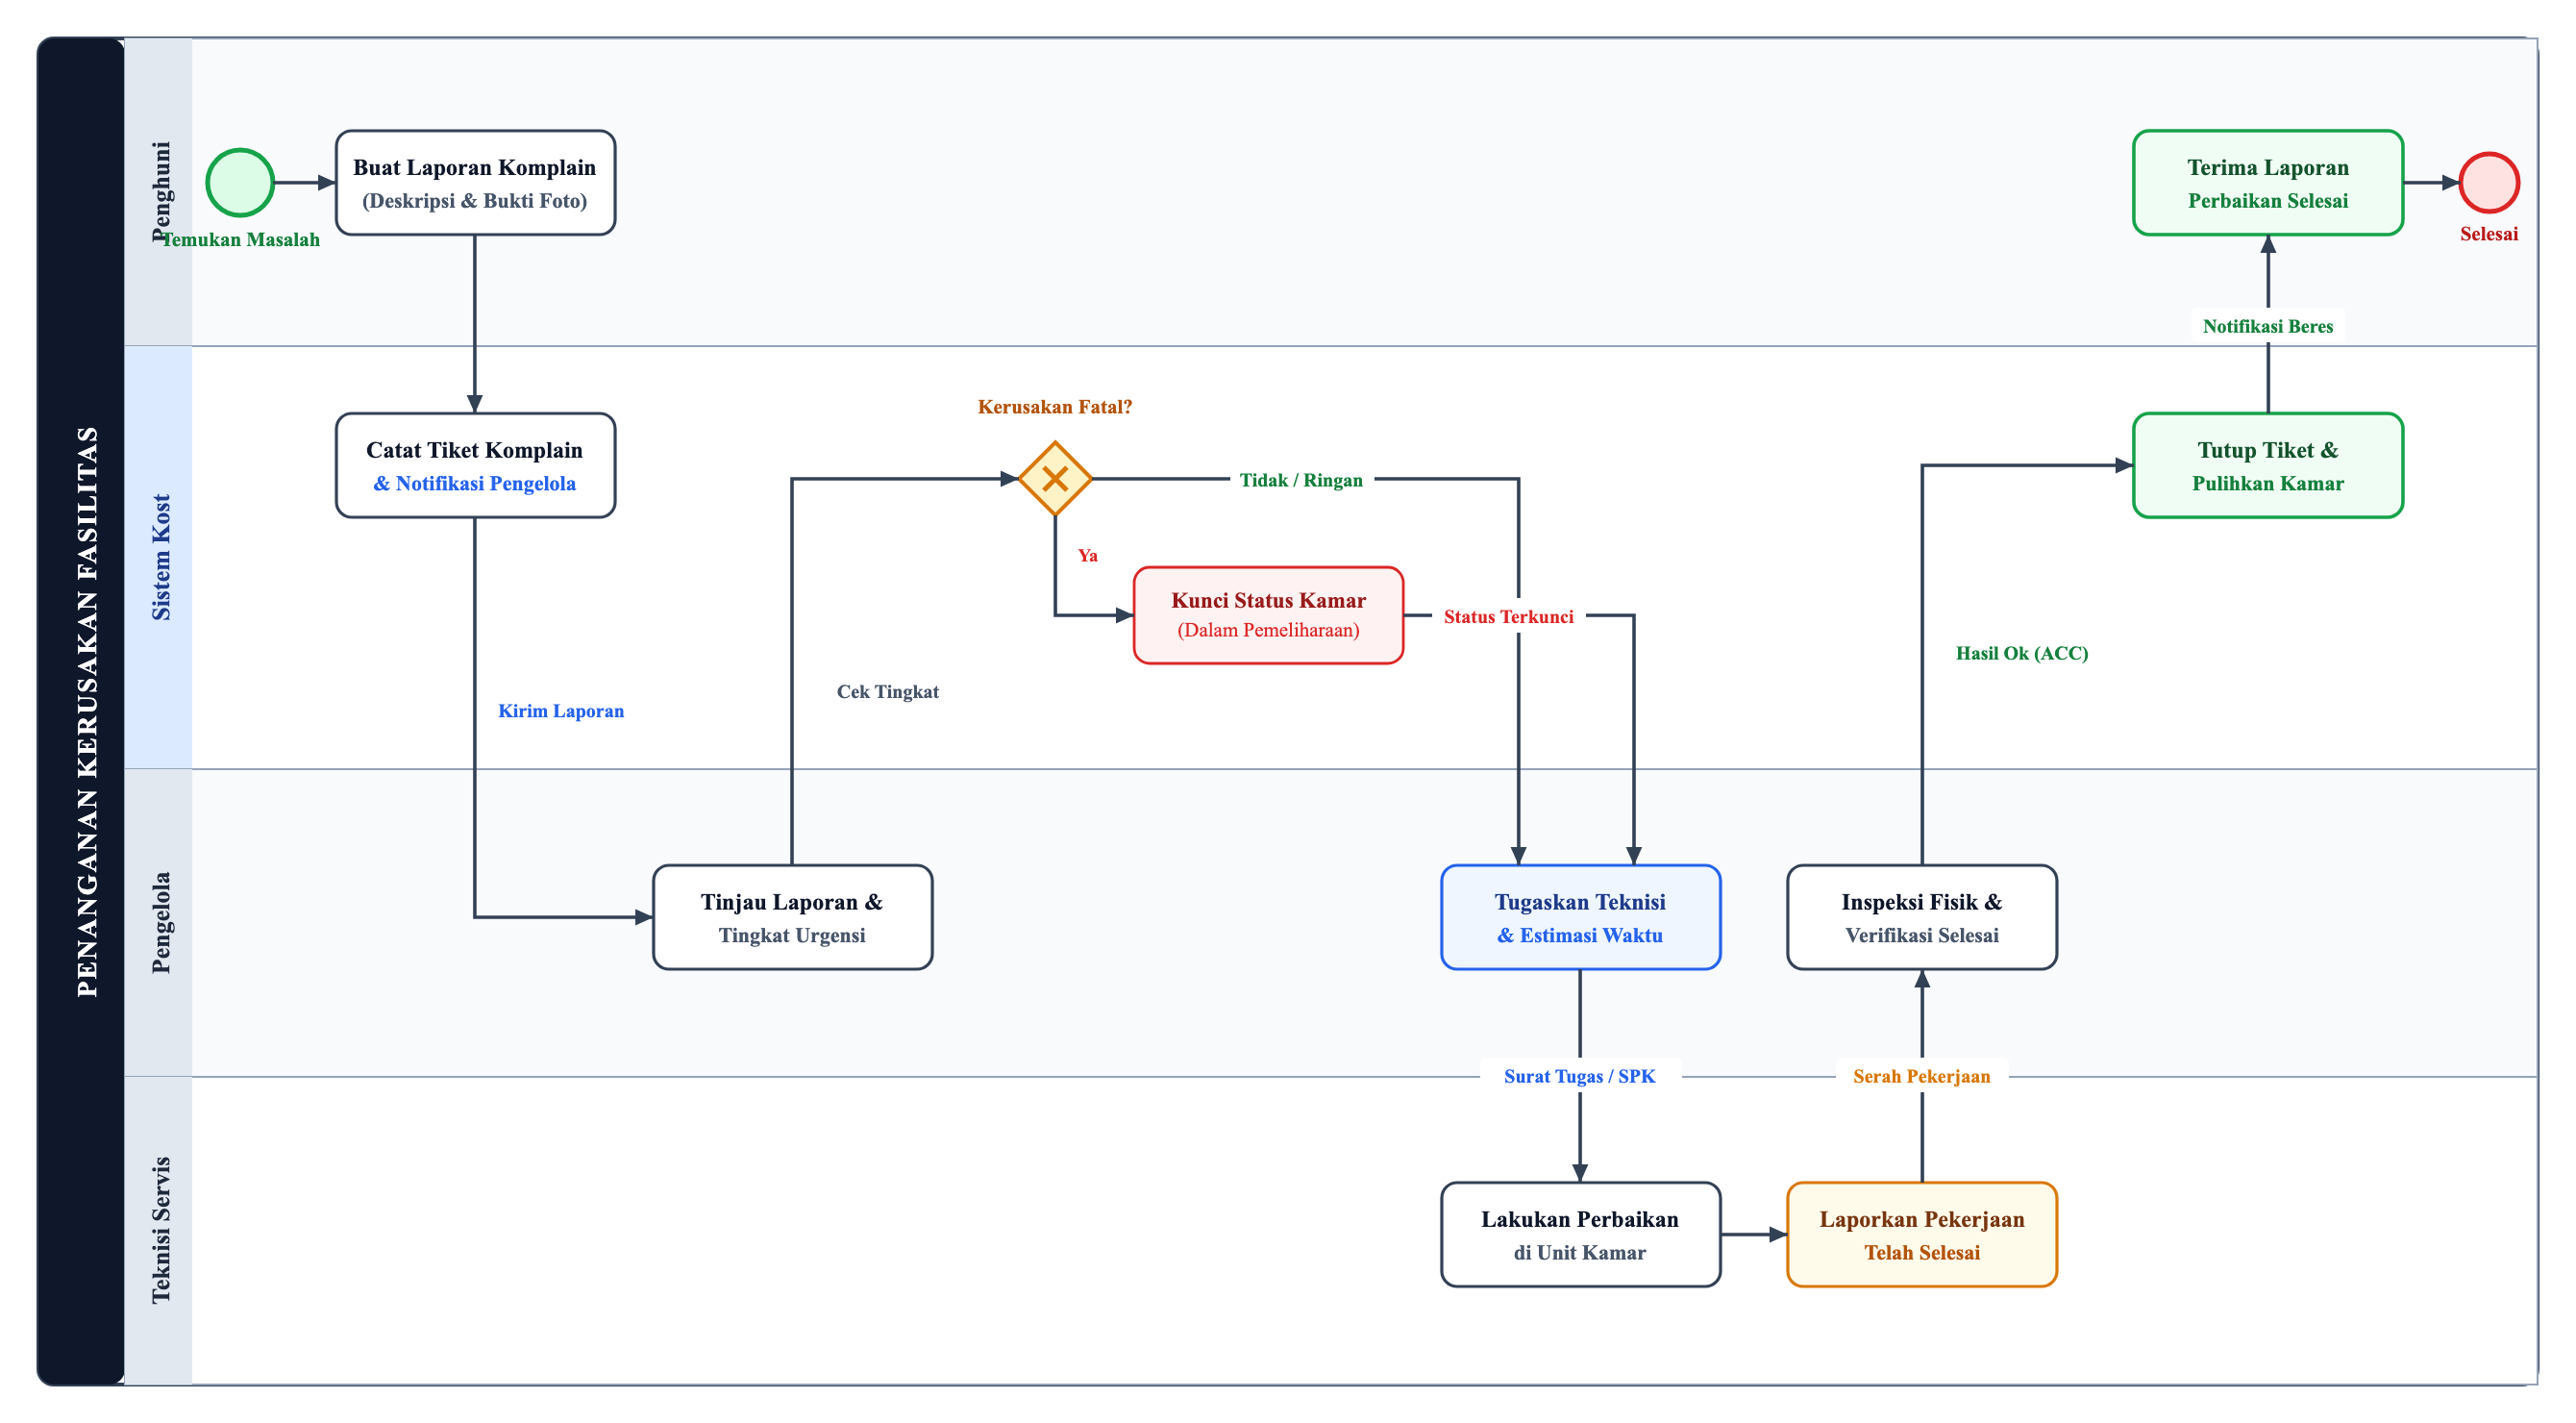
\includegraphics[width=0.96\textwidth,height=0.65\textheight,keepaspectratio]{assets/diagrams/bab3_07_alur_laporan_kerusakan.png}
  \caption{Diagram Alur Proses Penanganan Tiket Kerusakan Fasilitas}
  \label{fig:alur_kerusakan}
\end{figure}

Tahapan proses pada Gambar~\ref{fig:alur_kerusakan} meliputi:
\begin{enumerate}[label=\arabic*., leftmargin=*]
  \item Penghuni mengisi formulir komplain pada portal web, melampirkan deskripsi masalah dan foto bukti kerusakan (\texttt{POST /api/damage-reports}).
  \item Modul Maintenance menyimpan laporan pada tabel \texttt{damage\_reports} dengan status \texttt{open} dan memancarkan event \texttt{RoomDamaged}.
  \item Jika kerusakan tergolong fatal dan unit tidak layak huni sementara waktu, modul Room memperbarui status kamar menjadi \texttt{maintenance} agar terkunci dari alokasi baru.
  \item Pengelola menerima daftar tiket baru pada dasbor operasional, meninjau foto bukti, lalu menugaskan teknisi dengan mengubah status tiket menjadi \texttt{in\_progress}.
  \item Teknisi melakukan perbaikan fisik di lokasi. Setelah selesai, pengelola atau teknisi menutup tiket (\texttt{POST /api/damage-reports/\{id\}/resolve}) dengan melampirkan foto hasil perbaikan dan catatan teknis.
  \item Modul Maintenance memancarkan event \texttt{RoomRepaired}. Modul Room mengembalikan status kamar menjadi \texttt{kosong} (atau tetap \texttt{terisi} jika penghuni masih menghuni), dan modul Notification mengirim pemberitahuan penyelesaian perbaikan kepada penghuni.
\end{enumerate}

\subsection{Alur Pemeliharaan Rutin Berkala}

Alur ini mencakup agenda perawatan preventif fasilitas umum gedung (misalnya servis AC rutin, pembersihan tandon air, atau penyemprotan hama) yang dijalankan berdasarkan jadwal kalender, seperti ditunjukkan pada Gambar~\ref{fig:alur_pemeliharaan}.

\begin{figure}[H]
  \centering
  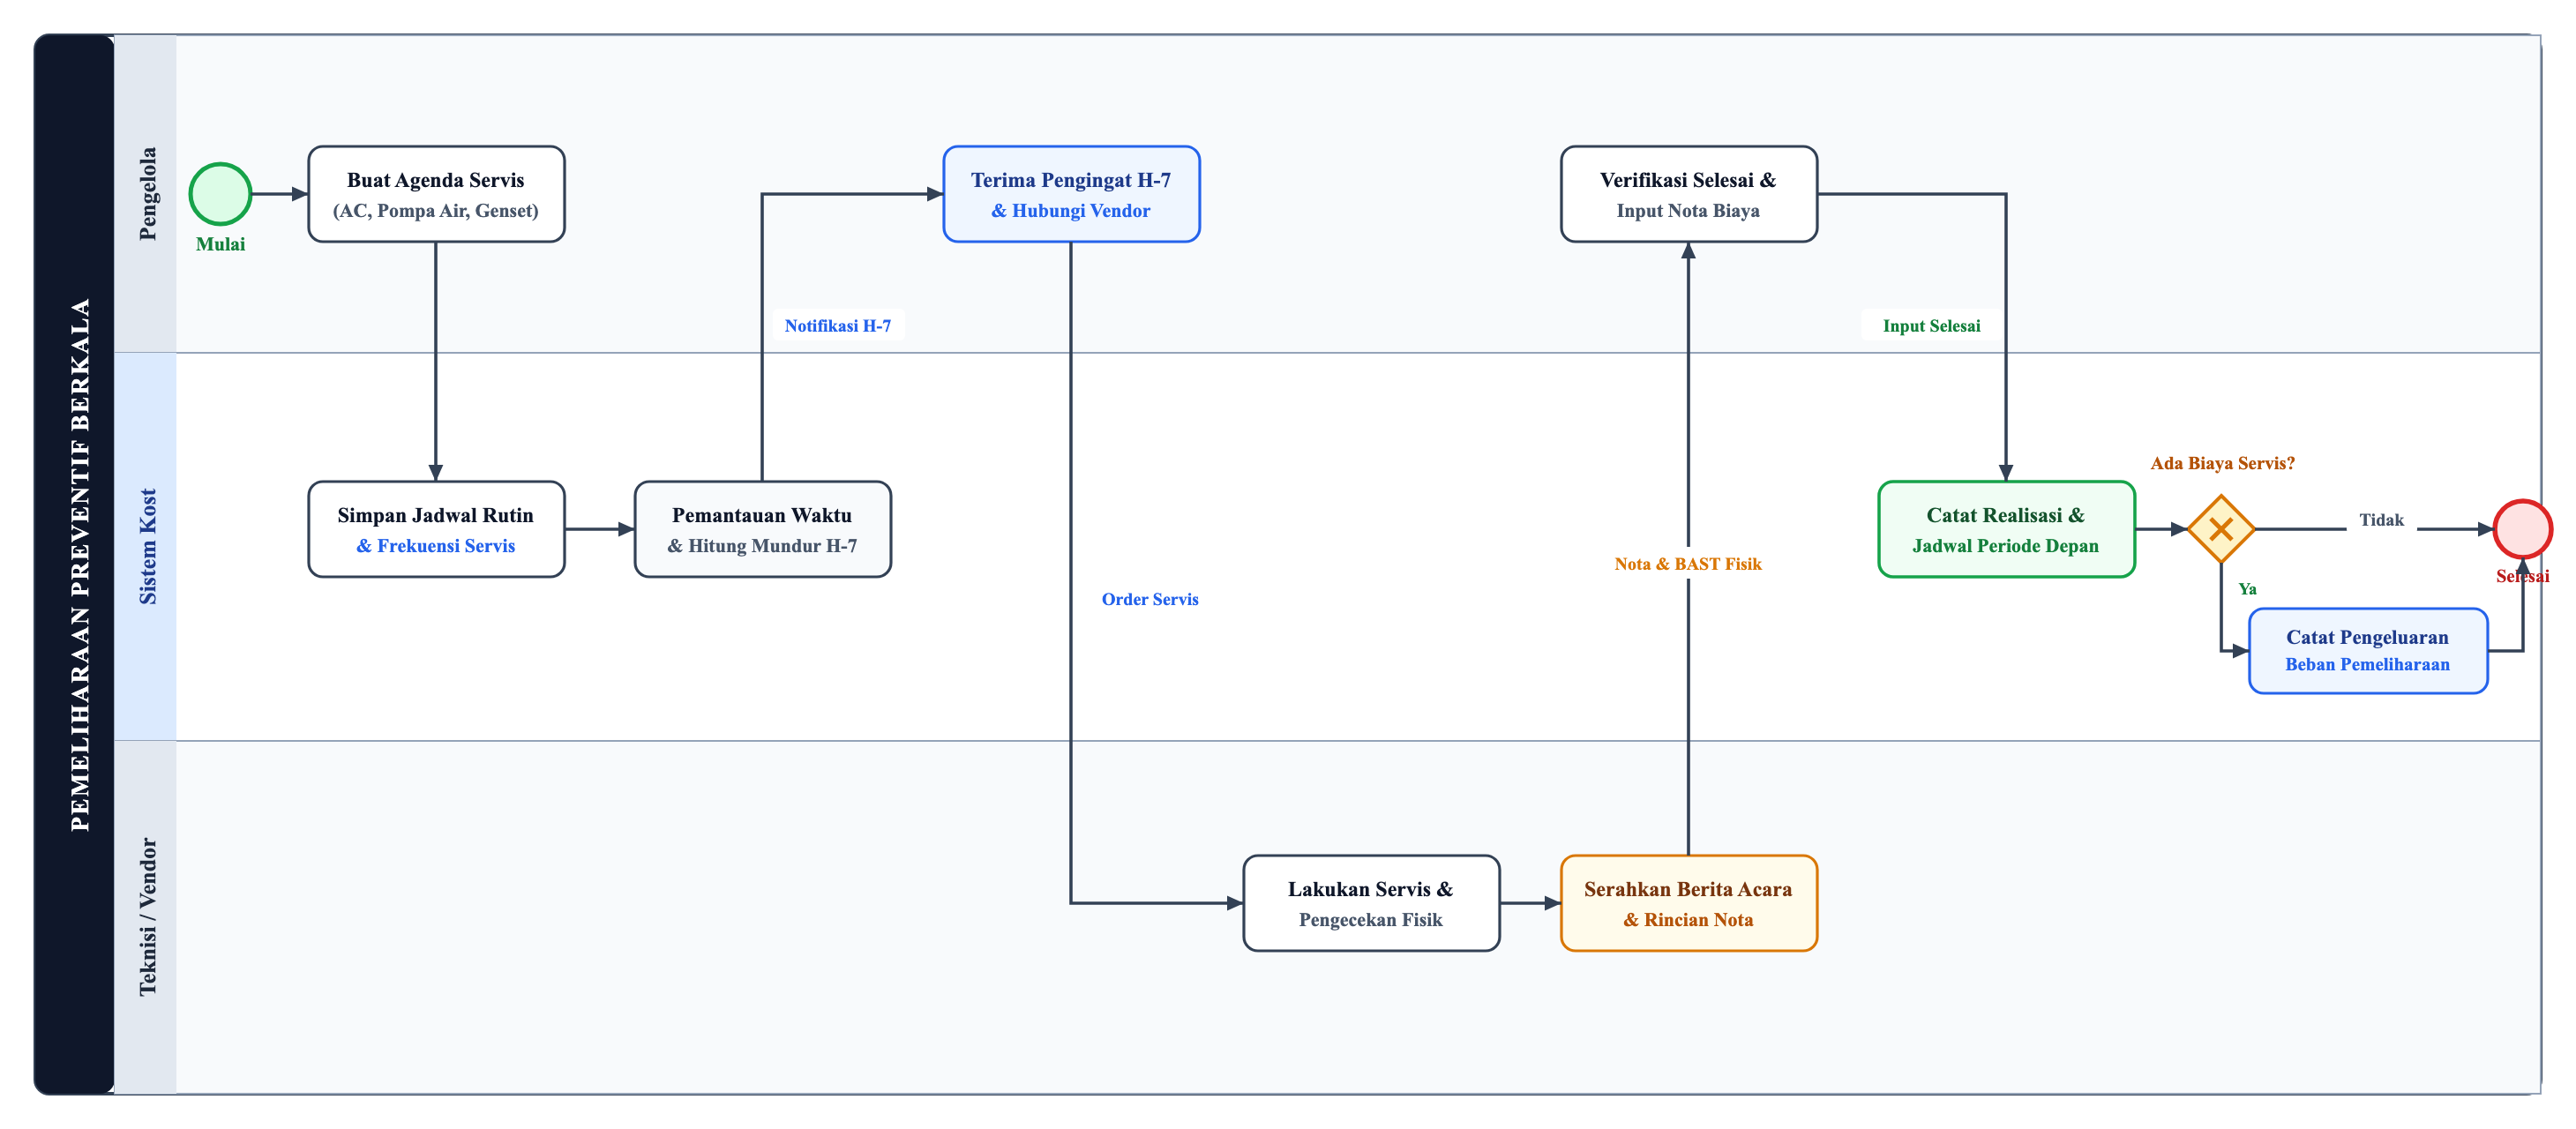
\includegraphics[width=0.96\textwidth,height=0.65\textheight,keepaspectratio]{assets/diagrams/bab3_08_alur_pemeliharaan_rutin.png}
  \caption{Diagram Alur Proses Pemeliharaan Rutin Berkala}
  \label{fig:alur_pemeliharaan}
\end{figure}

Tahapan proses pada Gambar~\ref{fig:alur_pemeliharaan} meliputi:
\begin{enumerate}[label=\arabic*., leftmargin=*]
  \item Pengelola mendaftarkan jadwal servis preventif pada kalender operasional dengan menetapkan jenis fasilitas, periode interval (misalnya setiap 3 bulan), dan tanggal jatuh tempo perawatan berikutnya.
  \item Penjadwal latar belakang memeriksa kalender secara harian. Saat waktu memasuki H-7 sebelum jadwal jatuh tempo, sistem memicu pengingat otomatis di dasbor pengelola dan mengirimkan pesan WhatsApp ke teknisi penanggung jawab.
  \item Teknisi melaksanakan servis fisik pada tanggal yang ditentukan.
  \item Setelah pekerjaan selesai, pengelola mencatat realisasi servis pada sistem, memasukkan biaya riil yang timbul, dan menandai status perawatan menjadi \texttt{completed}.
  \item Modul Maintenance menerbitkan event \texttt{MaintenanceServiceCompleted} ke modul Finance agar total biaya perawatan dapat dibukukan sebagai pengeluaran operasional gedung.
\end{enumerate}

\subsection{Alur Pencatatan Pengeluaran Operasional}

Alur ini mengatur tata kelola pengeluaran kas operasional gedung demi menjamin akuntabilitas pembukuan keuangan dan menghasilkan kalkulasi laba bersih secara riil (Gambar~\ref{fig:alur_pengeluaran}).

\begin{figure}[H]
  \centering
  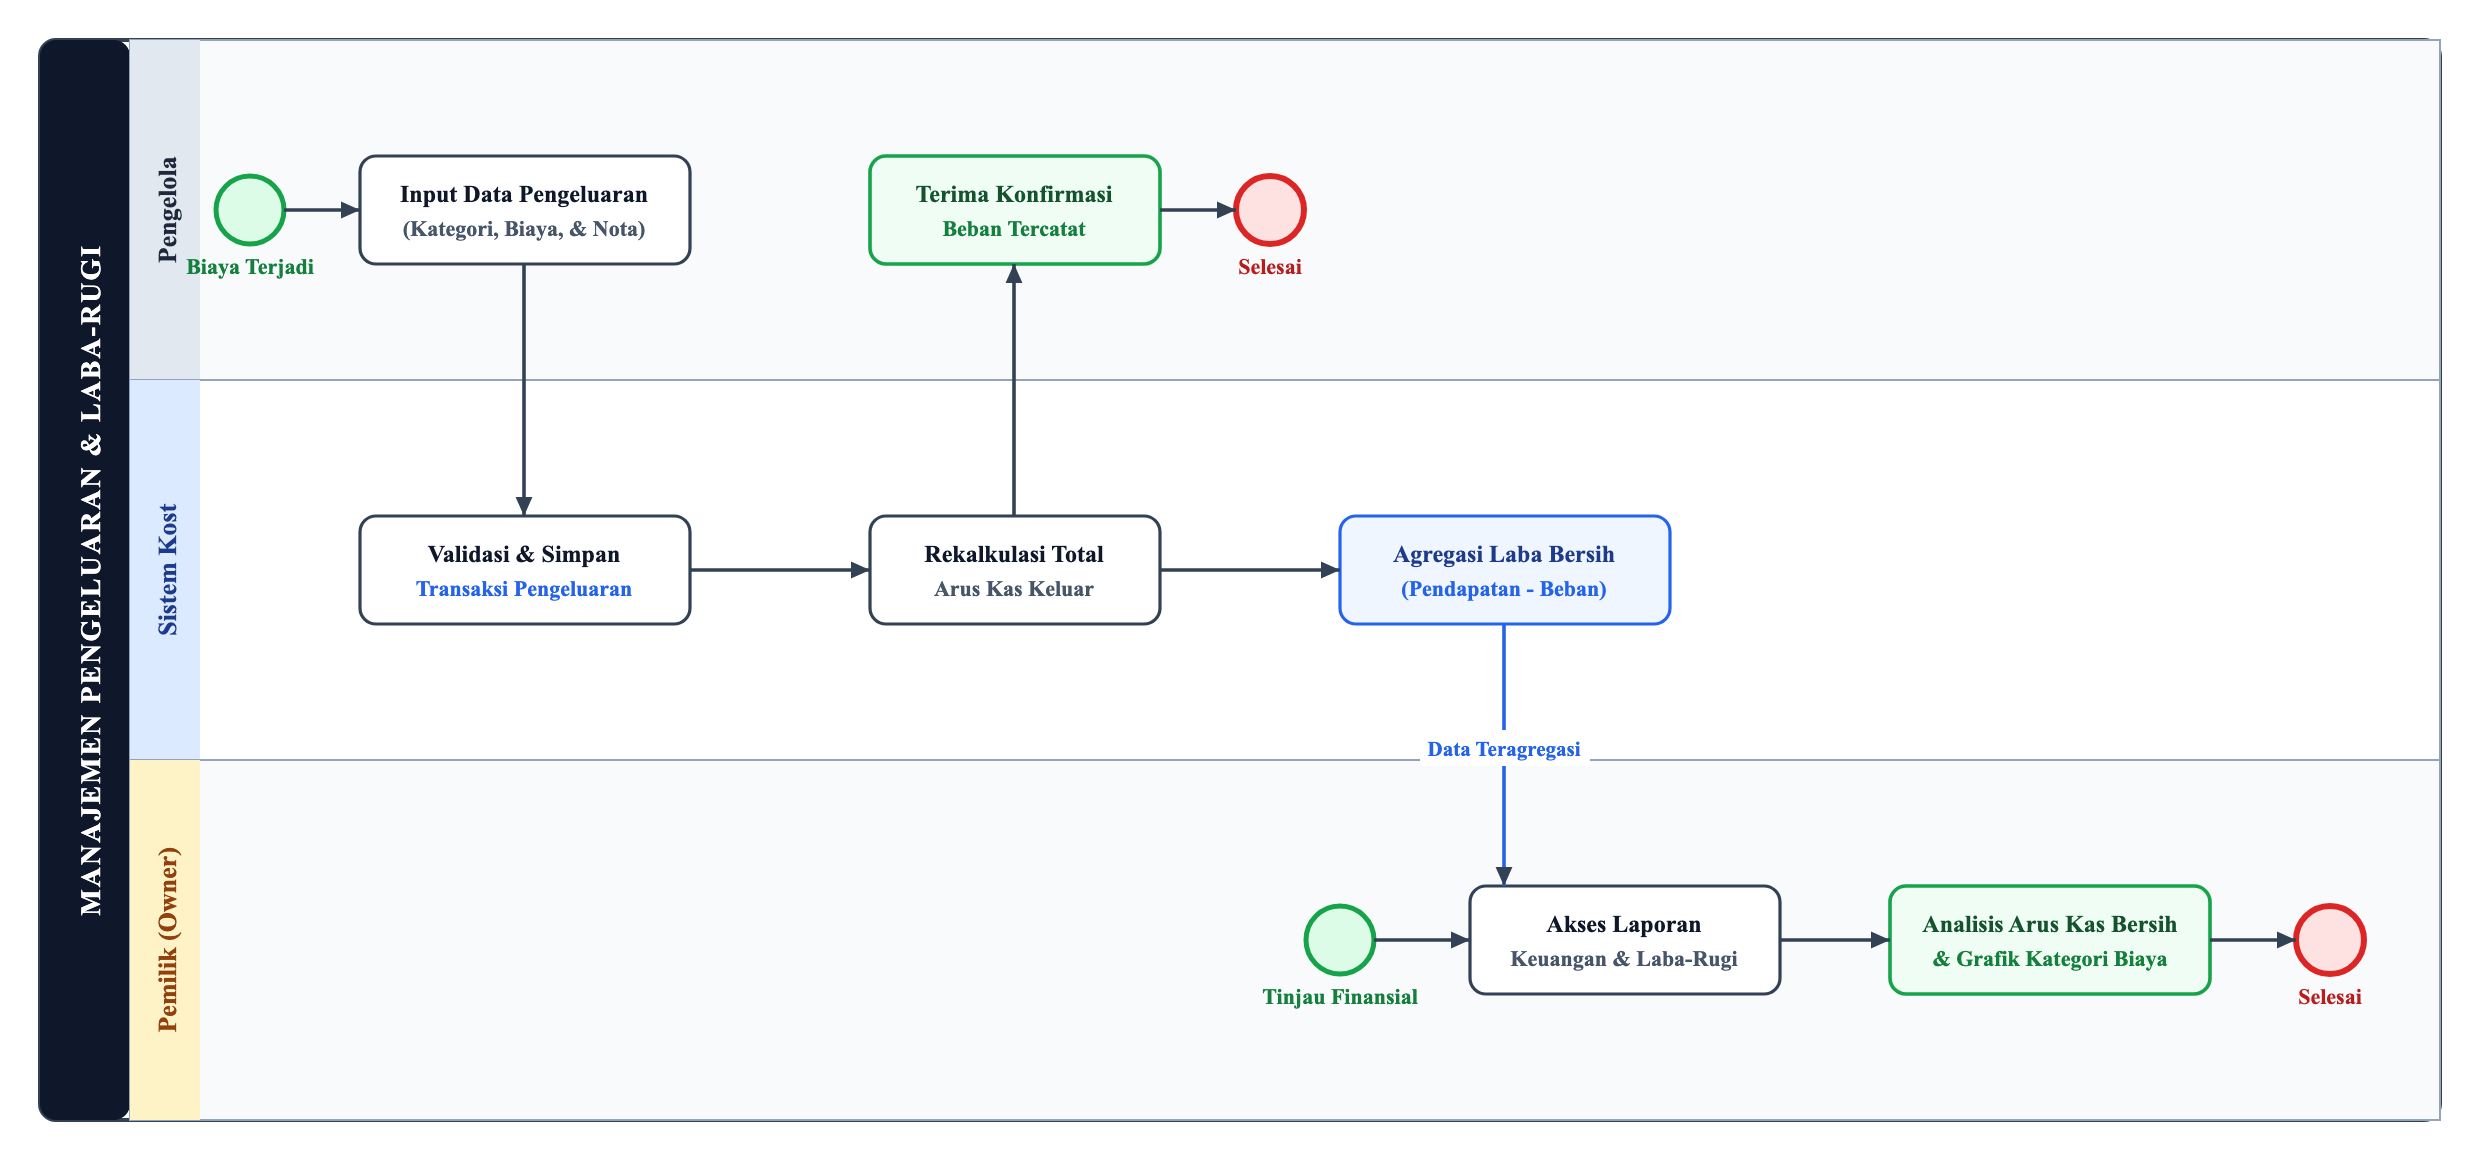
\includegraphics[width=0.96\textwidth,height=0.65\textheight,keepaspectratio]{assets/diagrams/bab3_09_alur_pengeluaran_operasional.png}
  \caption{Diagram Alur Proses Pencatatan Pengeluaran Operasional}
  \label{fig:alur_pengeluaran}
\end{figure}

Tahapan proses pada Gambar~\ref{fig:alur_pengeluaran} meliputi:
\begin{enumerate}[label=\arabic*., leftmargin=*]
  \item Pengelola mengeluarkan kas untuk kebutuhan gedung (seperti pembayaran listrik PLN, tagihan air PDAM, langganan internet, pembelian perlengkapan kebersihan, atau upah teknisi).
  \item Pengelola membuka menu pengeluaran pada dasbor web, memilih kategori biaya, mengisi nominal, serta mengunggah foto nota fisik atau kuitansi pembayaran.
  \item Modul Finance memvalidasi kelengkapan data dan menyimpan rekaman transaksi kas keluar.
  \item Sistem secara otomatis menghitung laba bersih (\textit{Net Operating Income}) gedung dengan mengurangkan total pengeluaran operasional dari seluruh penerimaan sewa dan denda pada periode berjalan.
  \item Laporan arus kas dan grafik rekapitulasi laba bersih langsung tersaji pada Dasbor Pemilik secara \textit{real-time}.
\end{enumerate}

\subsection{Alur Pengawasan Buku Tamu}

Alur ini memfasilitasi pencatatan kunjungan tamu dari luar demi menjaga ketertiban lingkungan gedung kost, mencakup pra-registrasi, konfirmasi kedatangan (\textit{check-in}), kepulangan (\textit{check-out}), serta pengenaan biaya inap jika berlaku (Gambar~\ref{fig:alur_tamu}).

\begin{figure}[H]
  \centering
  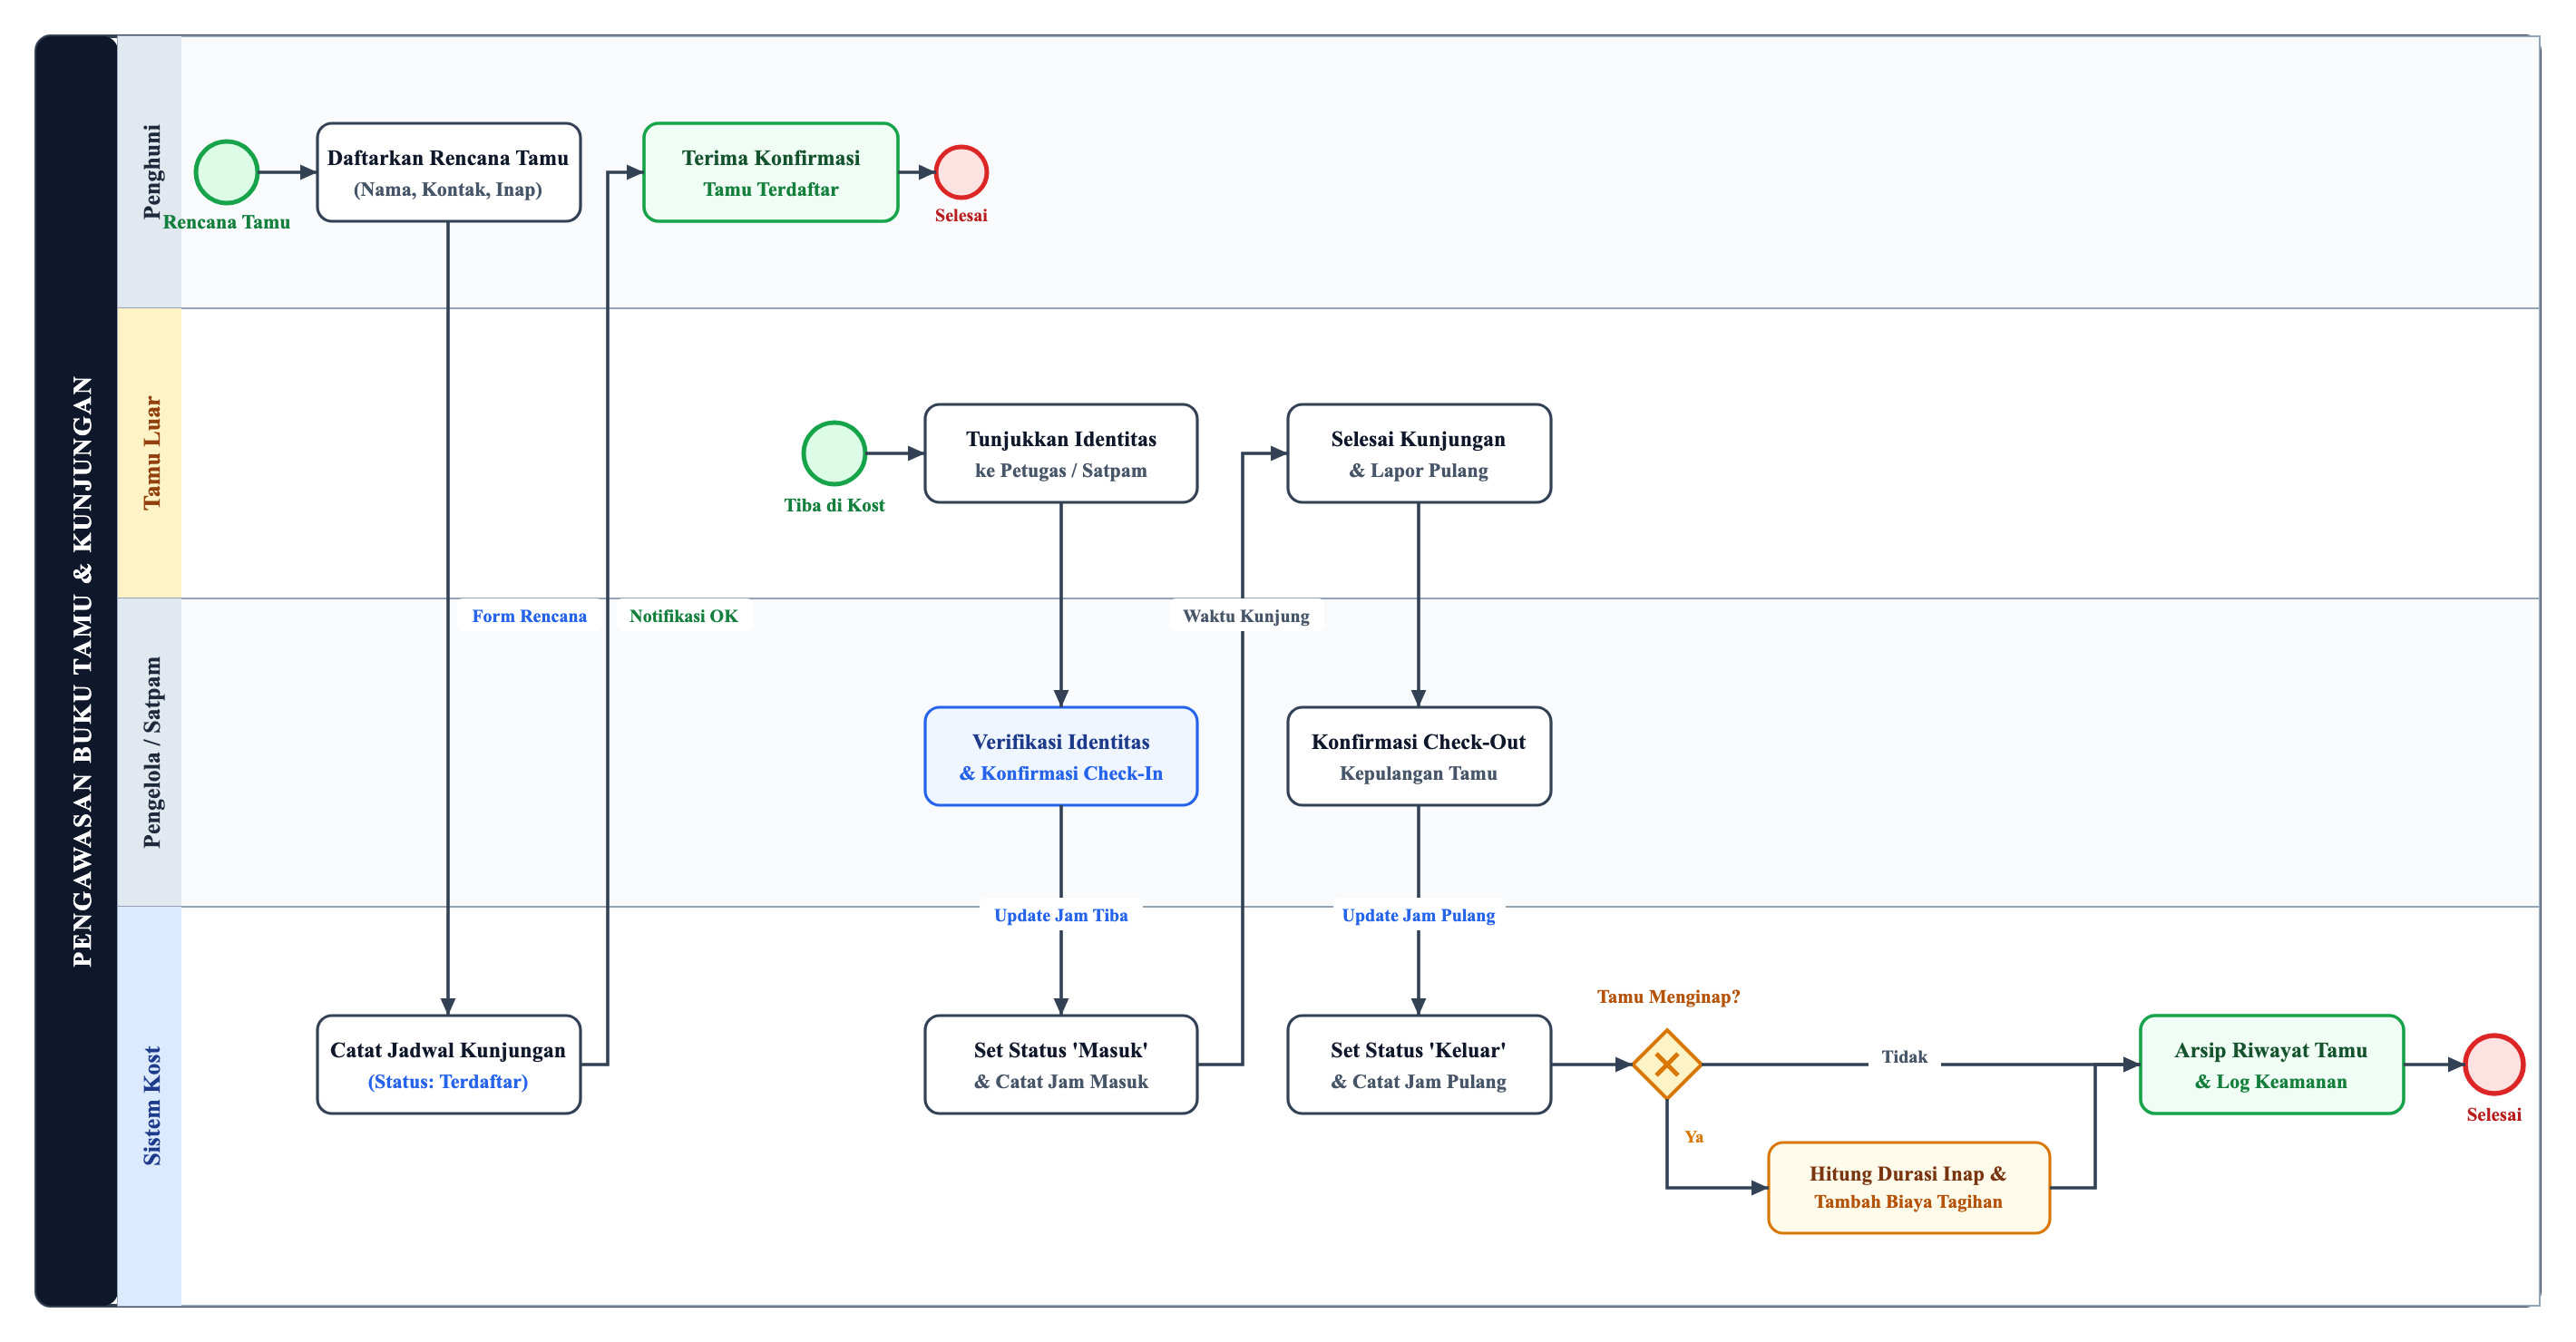
\includegraphics[width=0.96\textwidth,height=0.65\textheight,keepaspectratio]{assets/diagrams/bab3_10_alur_pengawasan_buku_tamu.png}
  \caption{Diagram Alur Proses Pengawasan Buku Tamu}
  \label{fig:alur_tamu}
\end{figure}

Tahapan proses pada Gambar~\ref{fig:alur_tamu} meliputi:
\begin{enumerate}[label=\arabic*., leftmargin=*]
  \item Penghuni mendaftarkan tamu yang akan datang berkunjung melalui portal web (\texttt{POST /api/guests}), mengisi nama tamu, kontak, dan perkiraan waktu berkunjung.
  \item Saat tamu tiba di lokasi gedung, pengelola atau petugas keamanan memverifikasi identitas fisik tamu dan menekan tombol konfirmasi kehadiran (\textit{check-in}).
  \item Ketika tamu selesai berkunjung dan meninggalkan lokasi, petugas mencatat waktu kepulangan fisik (\textit{check-out}). Modul Guest memperbarui status kunjungan menjadi \texttt{checked\_out} dan memancarkan event \texttt{GuestCheckedOut}.
  \item Jika tamu menginap melewati batas jam malam dan gedung menerapkan kebijakan tarif tamu menginap (\texttt{guest\_fee\_enabled = true}), modul Guest menghitung jumlah malam menginap dan meneruskan data biaya tersebut ke modul Finance untuk dimasukkan ke dalam invoice tagihan berkala penghuni yang bersangkutan.
\end{enumerate}

\subsection{Alur Pengaturan Hak Akses Dinamis (Dynamic RBAC)}

Alur ini memungkinkan Pemilik untuk menyusun peran kerja staf (\textit{custom roles}) secara mandiri dengan mencentang kumpulan izin modular (\textit{granular permissions}) tanpa perlu melakukan perubahan kode sumber aplikasi (Gambar~\ref{fig:alur_rbac}).

\begin{figure}[H]
  \centering
  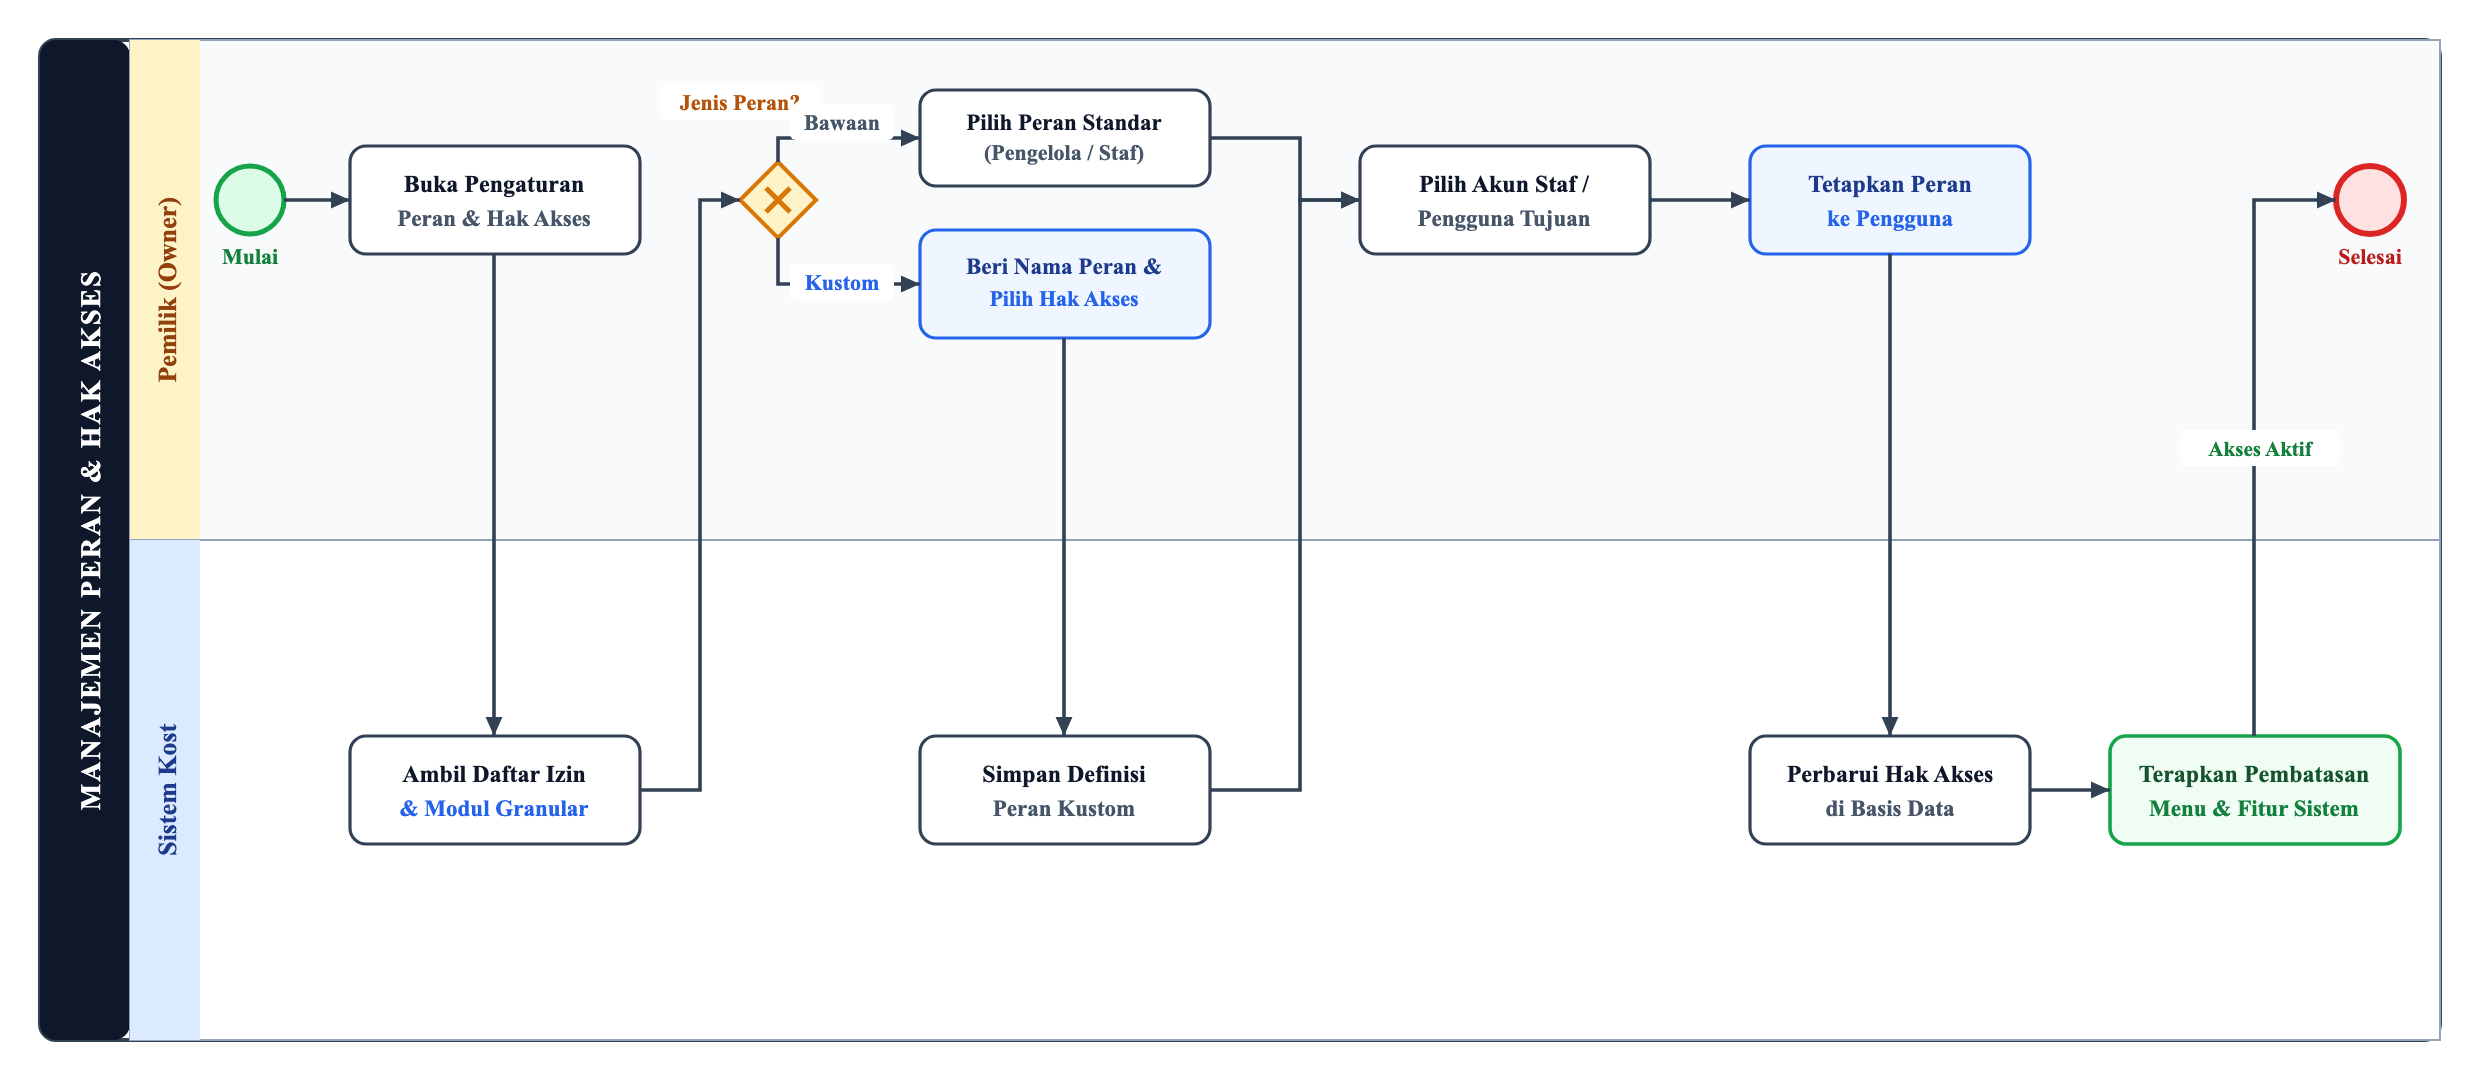
\includegraphics[width=0.96\textwidth,height=0.65\textheight,keepaspectratio]{assets/diagrams/bab3_11_alur_hak_akses_dinamis.png}
  \caption{Diagram Alur Proses Pengaturan Hak Akses Dinamis}
  \label{fig:alur_rbac}
\end{figure}

Tahapan proses pada Gambar~\ref{fig:alur_rbac} meliputi:
\begin{enumerate}[label=\arabic*., leftmargin=*]
  \item Pemilik membuka menu pengaturan peran dan izin pada dasbor web.
  \item Sistem menyajikan daftar hak akses granular yang tersedia di setiap modul (seperti \texttt{room:read}, \texttt{room:write}, \texttt{finance:view\_invoice}, \texttt{maintenance:update\_ticket}).
  \item Pemilik dapat memilih antara memakai peran standar bawaan (\texttt{owner}, \texttt{admin}, \texttt{resident}) atau membuat peran baru.
  \item Jika membuat peran baru, Pemilik memasukkan nama jabatan (contoh: ``Wali Asrama'' atau ``Petugas Keamanan''), mencentang hak akses yang ingin diberikan, lalu menyimpannya ke basis data.
  \item Pemilik menautkan peran kustom tersebut ke akun pengguna staf yang ditunjuk.
  \item Guard API backend dan menu antarmuka Flutter Web secara otomatis menyesuaikan tampilan dan membatasi rute akses sesuai izin yang aktif pada pengguna tersebut.
\end{enumerate}

\subsection{Alur Pendataan dan Audit Inventaris Aset}

Alur ini mengatur inventarisasi perabotan dan barang fasilitas di dalam kamar, pelaksanaan audit fisik saat serah terima kunci, serta penanganan otomatis jika ditemukan barang rusak atau hilang (Gambar~\ref{fig:alur_inventaris}).

\begin{figure}[H]
  \centering
  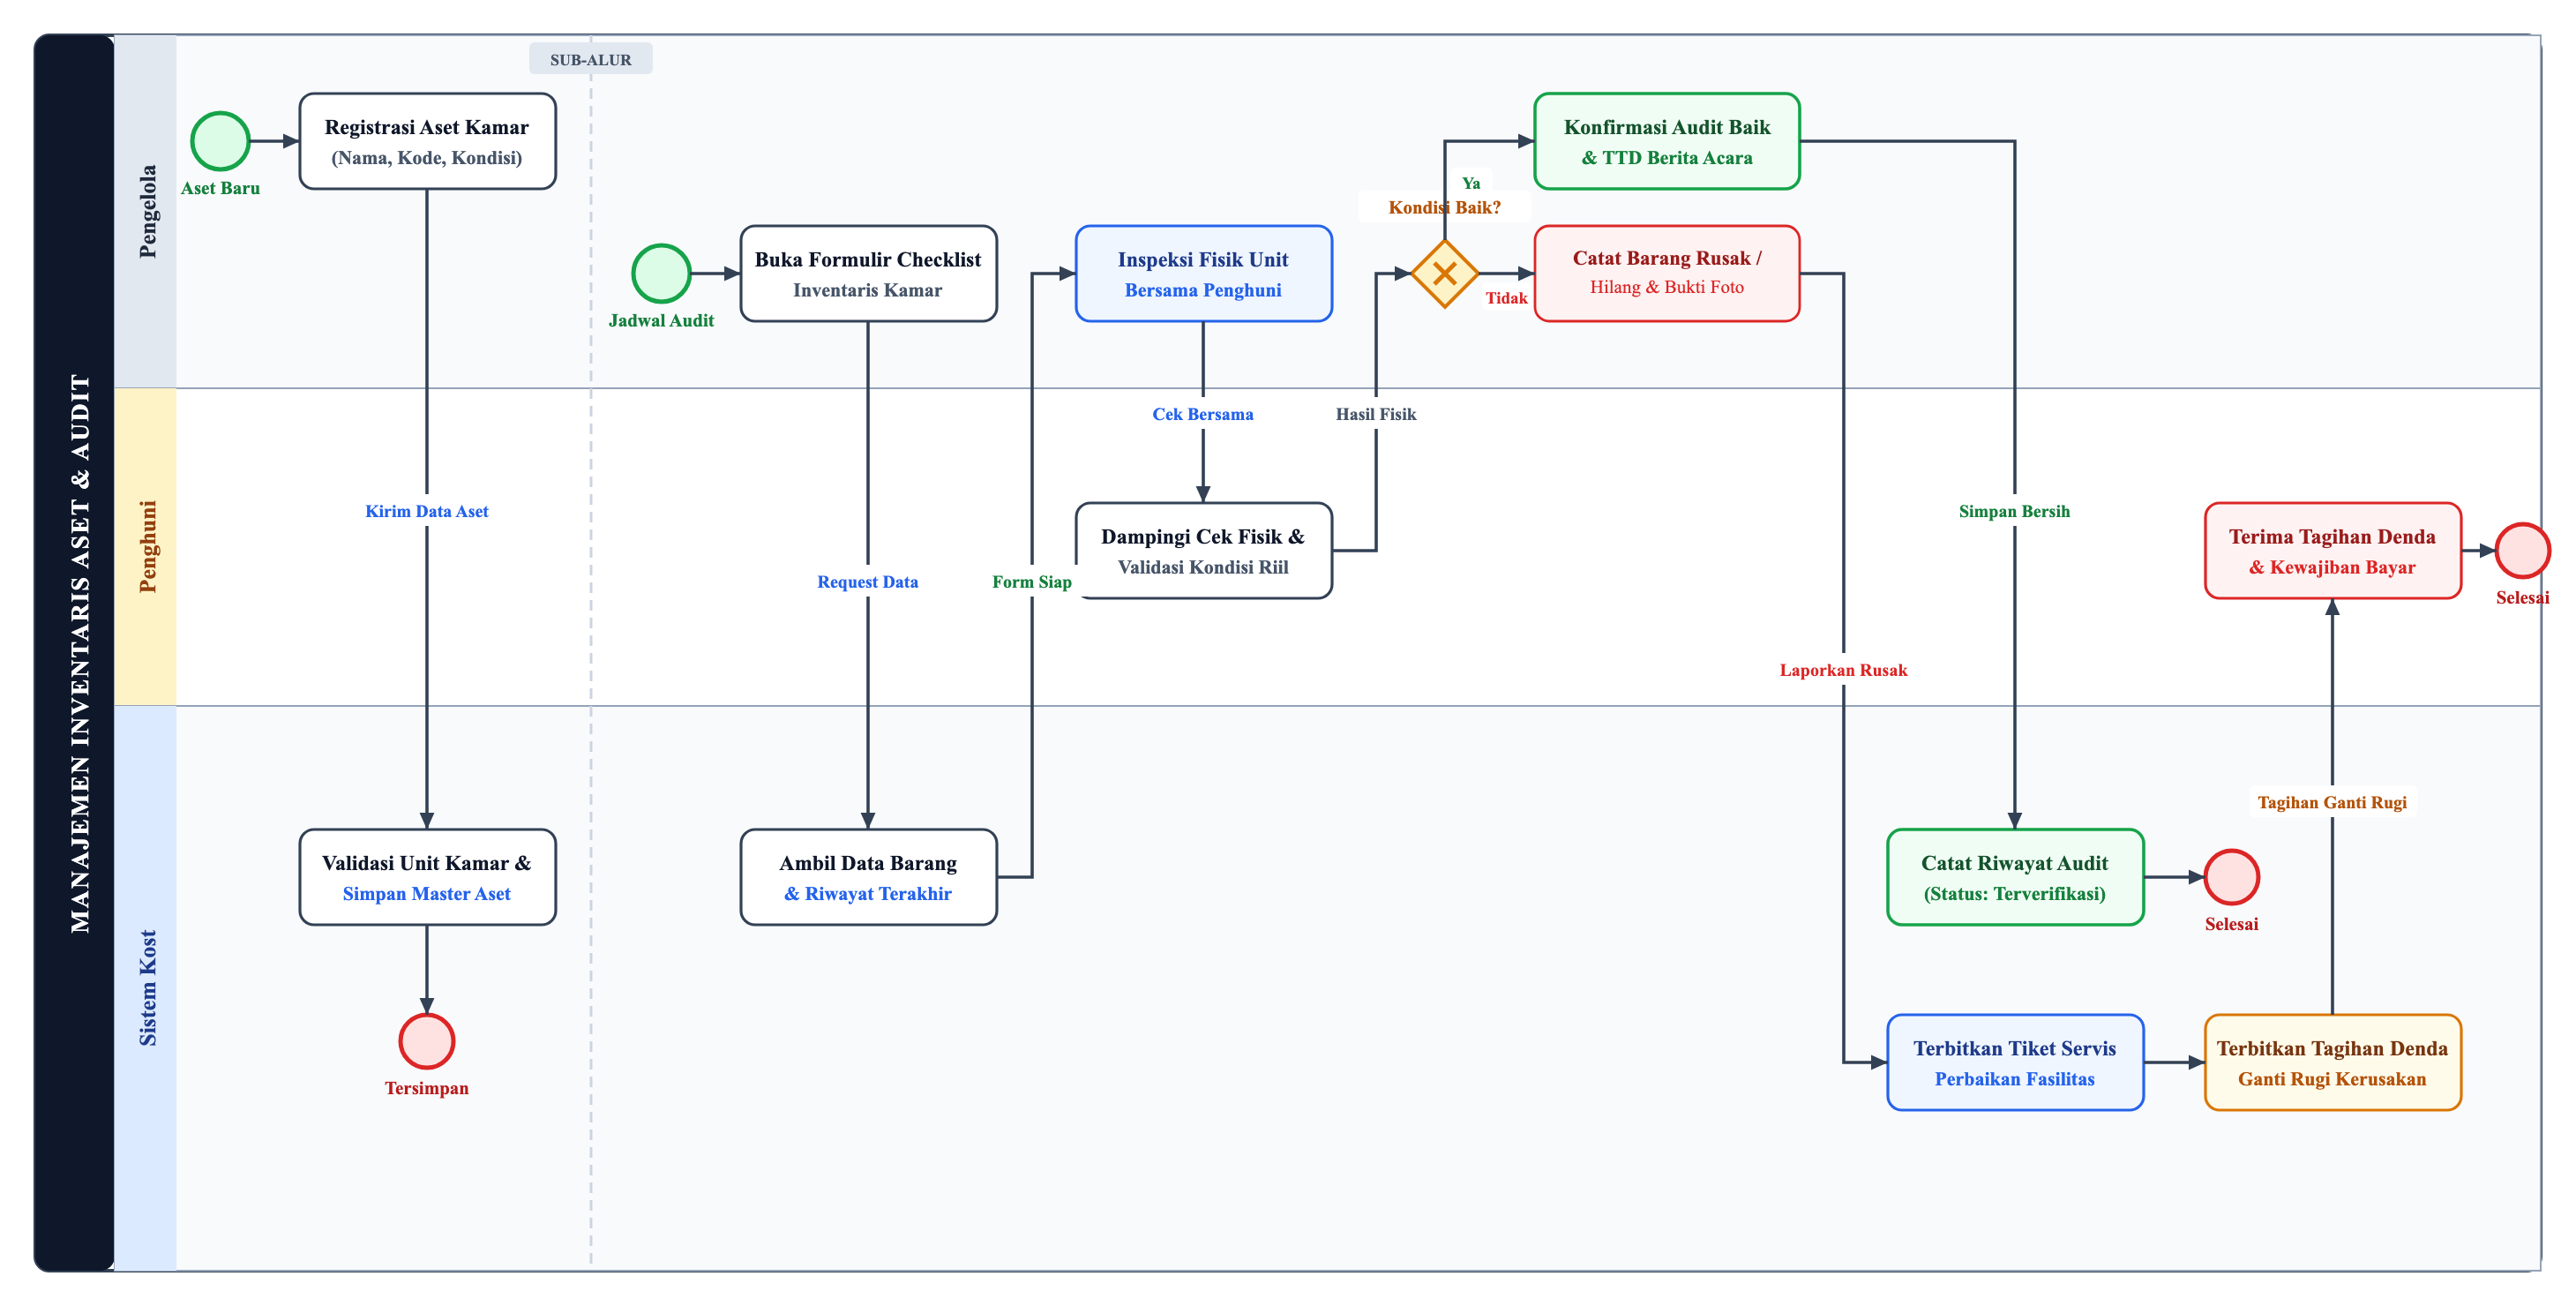
\includegraphics[width=0.96\textwidth,height=0.65\textheight,keepaspectratio]{assets/diagrams/bab3_12_alur_inventaris_aset.png}
  \caption{Diagram Alur Proses Pendataan dan Audit Inventaris Aset}
  \label{fig:alur_inventaris}
\end{figure}

Tahapan proses pada Gambar~\ref{fig:alur_inventaris} meliputi:
\begin{enumerate}[label=\arabic*., leftmargin=*]
  \item \textbf{Pendaftaran Aset:} Pengelola mendaftarkan barang aset ke modul Inventory (seperti kasur springbed, unit AC, lemari pakaian, meja belajar) lengkap dengan kode inventaris dan kondisi awal (\textit{baik}). Modul memvalidasi keberadaan unit kamar sebelum menyimpan rekaman aset.
  \item \textbf{Inspeksi Fisik (\textit{Check-in / Check-out}):} Saat terjadi serah terima kamar dengan penghuni, pengelola membuka lembar checklist inventaris pada aplikasi dan memeriksa kondisi barang bersama penghuni.
  \item \textbf{Hasil Verifikasi:}
    \begin{enumerate}[label=\alph*., leftmargin=*]
      \item Jika seluruh barang dalam kondisi lengkap dan baik, pengelola menandai audit sebagai \textit{verified}.
      \item Jika ditemukan barang yang rusak berat atau hilang, pengelola memperbarui kondisi aset menjadi \texttt{damaged} atau \texttt{lost}, lalu modul Inventory menerbitkan kejadian \texttt{AssetDamagedOrLost}.
    \end{enumerate}
  \item \textbf{Penanganan Insiden:}
    \begin{enumerate}[label=\alph*., leftmargin=*]
      \item Kejadian tersebut memicu modul Maintenance untuk menerbitkan tiket perbaikan fasilitas secara otomatis.
      \item Jika kerusakan disebabkan oleh kelalaian penghuni, modul Finance dapat menerbitkan tagihan penggantian kerugian aset ke dalam invoice penghuni yang bersangkutan.
    \end{enumerate}
\end{enumerate}

\subsection{Alur Konsultasi AI melalui Model Context Protocol (MCP)}

Alur ini mengatur bagaimana model kecerdasan buatan (LLM) dapat menjawab pertanyaan manajerial dari pemilik atau pengelola menggunakan data operasional yang faktual secara aman melalui protokol MCP (Gambar~\ref{fig:alur_mcp}).

\begin{figure}[H]
  \centering
  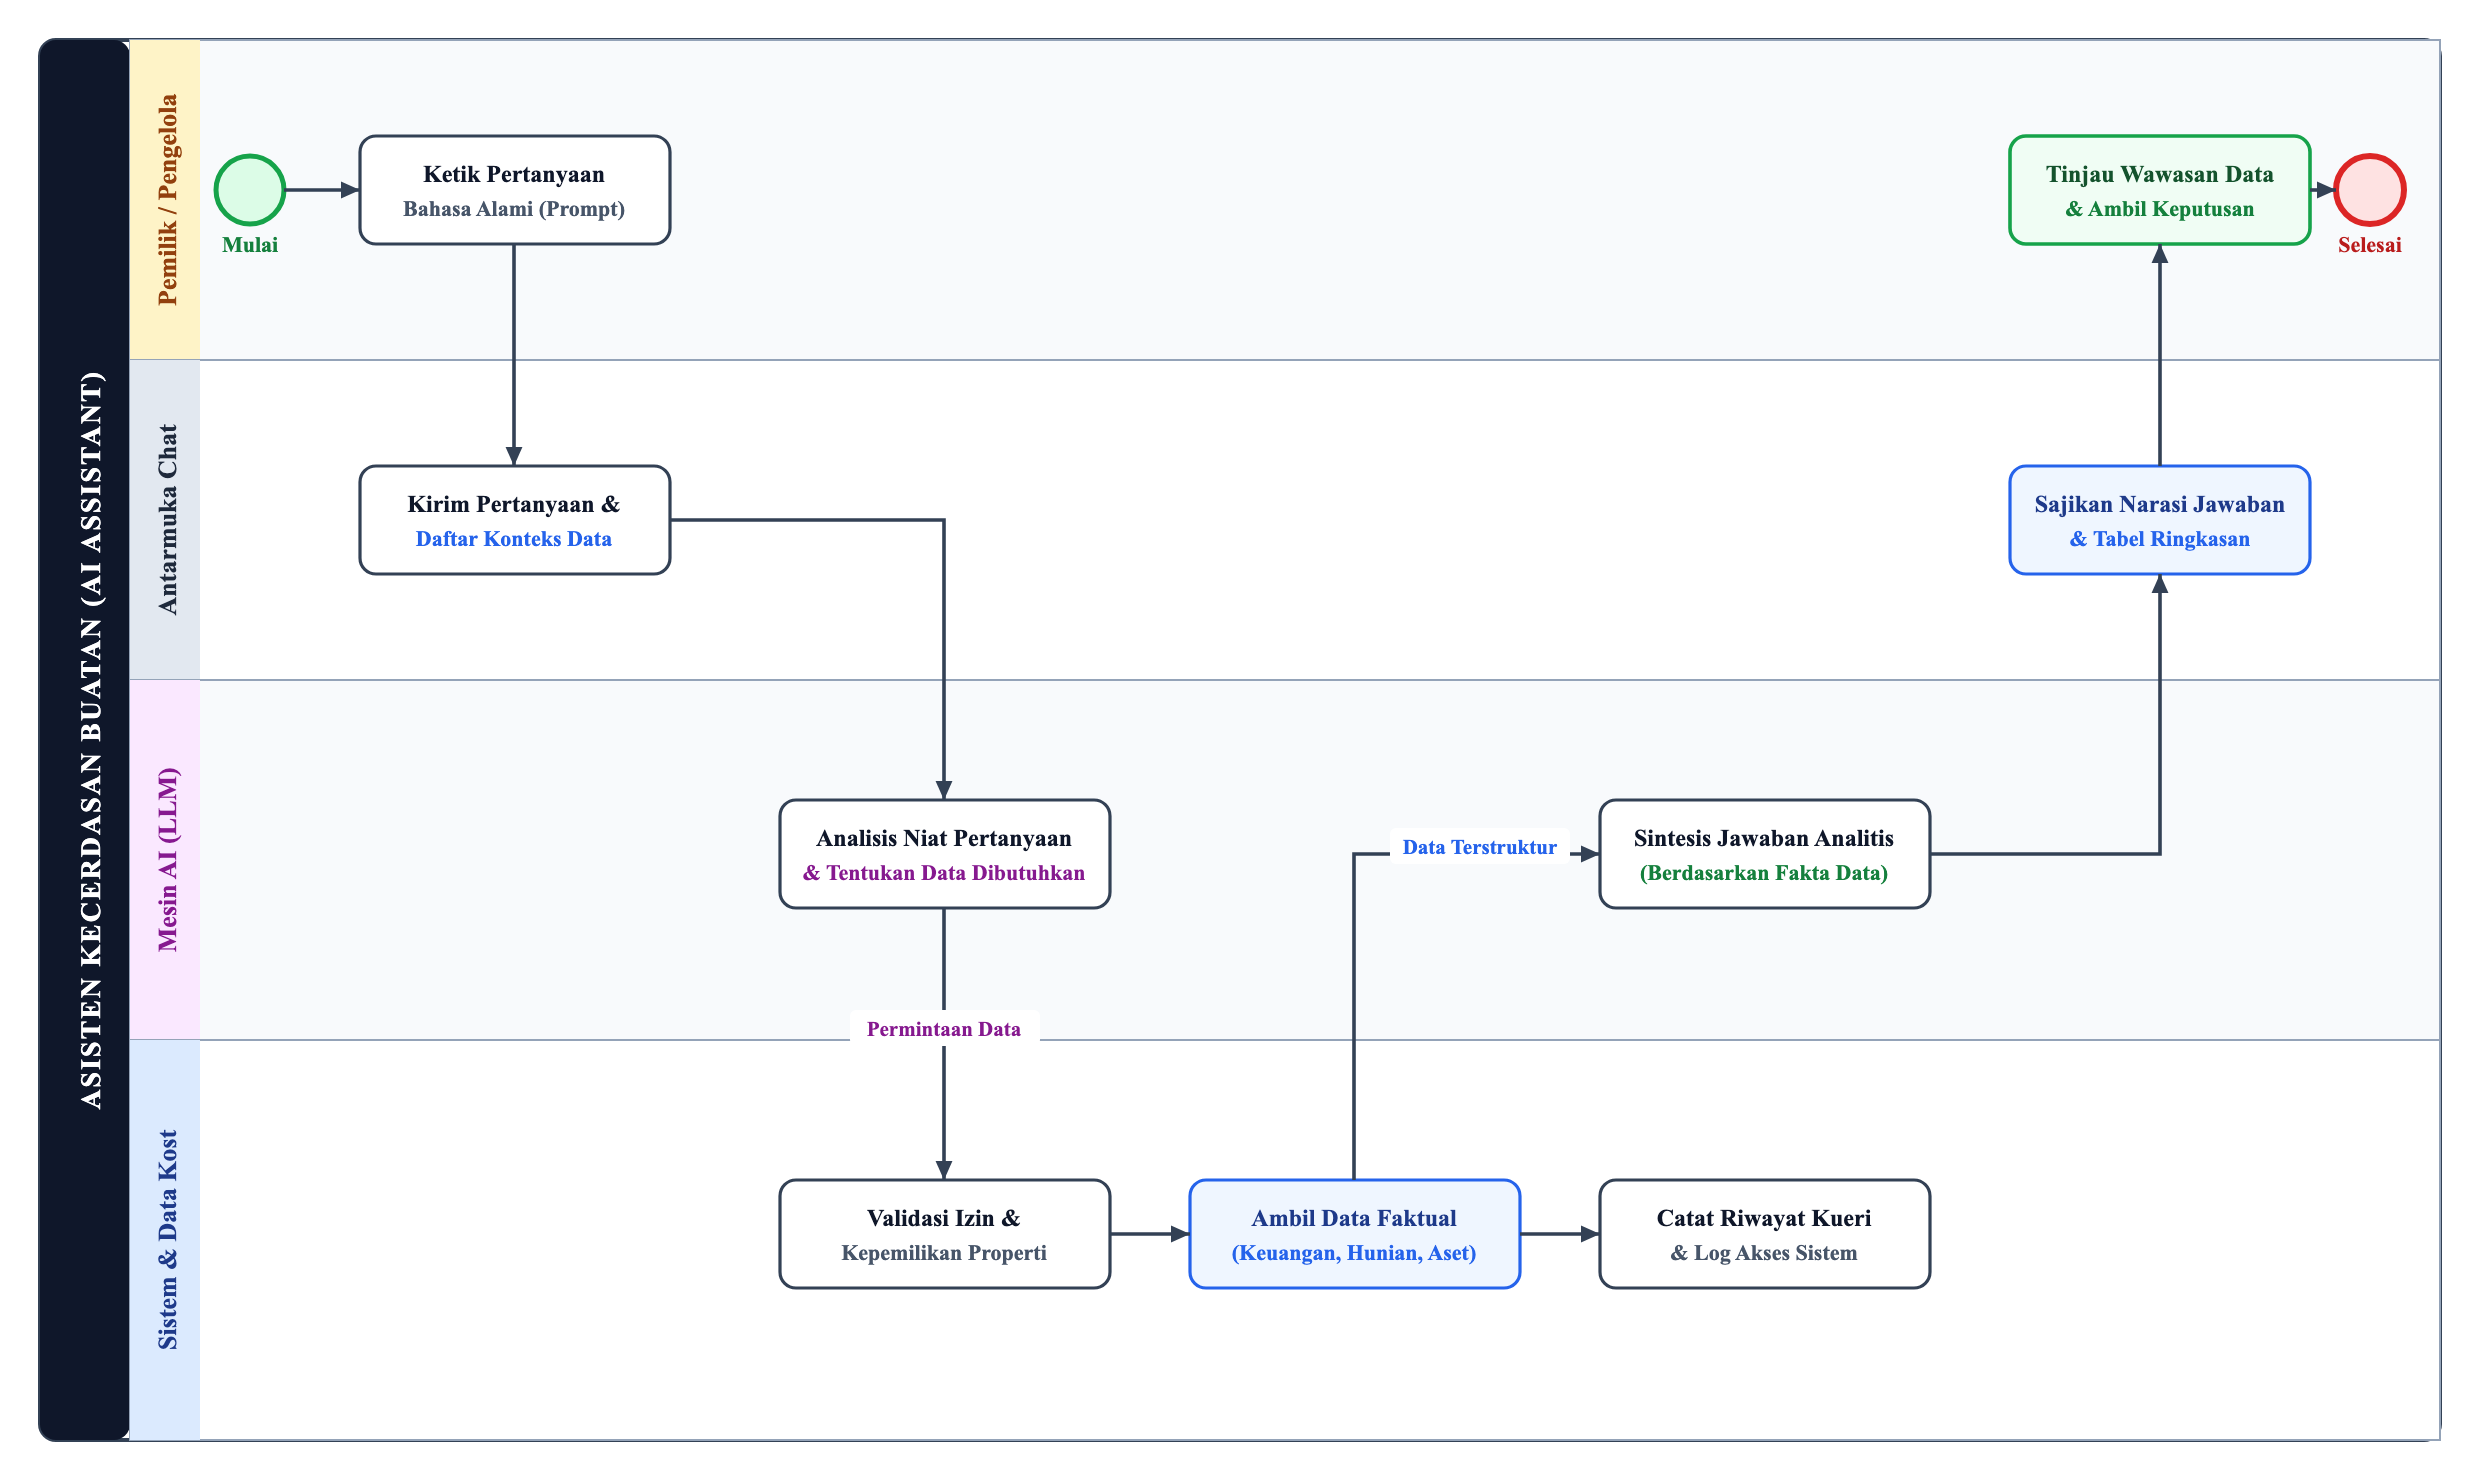
\includegraphics[width=0.96\textwidth,height=0.65\textheight,keepaspectratio]{assets/diagrams/bab3_13_alur_konsultasi_ai_mcp.png}
  \caption{Diagram Alur Proses Konsultasi AI melalui Model Context Protocol}
  \label{fig:alur_mcp}
\end{figure}

Tahapan proses pada Gambar~\ref{fig:alur_mcp} meliputi:
\begin{enumerate}[label=\arabic*., leftmargin=*]
  \item Pemilik atau pengelola menuliskan pertanyaan bahasa alami pada Tab Chat AI di antarmuka web (misalnya: ``Berapa total pendapatan Gedung Melati bulan ini?'').
  \item Klien antarmuka meneruskan pertanyaan tersebut beserta spesifikasi perkakas (\textit{tool schema}) ke mesin LLM.
  \item LLM menganalisis maksud pertanyaan dan menentukan alat baca yang tepat untuk dipanggil (misalnya \texttt{get\_financial\_summary}). LLM membalas ke antarmuka dengan permintaan eksekusi alat melalui protokol JSON-RPC 2.0.
  \item Antarmuka web memanggil endpoint MCP Server di backend (\texttt{POST /mcp/tools/call}).
  \item Modul MCP memverifikasi token pengguna dan memastikan bahwa pengguna memiliki hak akses sah terhadap properti yang ditanyakan (\texttt{building\_id}). Permintaan lintas tenant yang tidak berhak akan langsung ditolak.
  \item Modul MCP mengeksekusi kueri agregasi baca melalui \textit{Module Gateway} ke basis data PostgreSQL. Basis data mengembalikan data angka faktual murni.
  \item Modul MCP mencatat rekam jejak pemanggilan alat pada log audit aplikasi, lalu mengirimkan hasil JSON data faktual kembali ke LLM melalui antarmuka web.
  \item LLM merangkum data angka faktual tersebut menjadi jawaban bahasa alami yang jelas, terstruktur, dan bebas dari halusinasi (\textit{grounded data}). Antarmuka web menampilkan teks penjelasan beserta tabel ringkasan ke hadapan pengguna.
\end{enumerate}

\section{PEMODELAN FUNGSIONAL DAN ALIRAN DATA}

\subsection{Use Case Diagram}
\label{sec:use_case}

\textit{Use Case Diagram} memodelkan interaksi antara para pengguna sistem (\textit{aktor}) dengan fungsionalitas yang disediakan oleh sistem aplikasi manajemen rumah kost terpadu. Pemodelan ini mempertegas batasan kewenangan (\textit{role boundary}) antar-aktor sehingga setiap pengguna hanya dapat menjalankan fitur yang sesuai dengan peran dan cakupan propertinya.

Sistem melayani tiga kategori aktor manusia utama serta empat entitas sistem eksternal:
\begin{enumerate}[label=\arabic*., leftmargin=*]
  \item \textbf{Pemilik (\textit{Owner}):} Memiliki wewenang tertinggi untuk mendaftarkan gedung properti baru, mengatur kebijakan tarif huni, membuat peran staf kustom melalui \textit{Role Builder}, memantau dasbor performa portofolio bisnis seluruh gedung, serta mengajukan kueri analitik ke asisten AI.
  \item \textbf{Pengelola (\textit{Admin Gedung}):} Bertanggung jawab atas pengelolaan operasional harian pada satu gedung tertentu yang ditugaskan kepadanya. Pengelola mengelola ketersediaan unit kamar, memverifikasi permohonan sewa, menindaklanjuti tiket kerusakan fasilitas, mencatat pengeluaran kas operasional, mencatat buku tamu, serta melakukan audit inventaris kamar.
  \item \textbf{Penghuni (\textit{Resident}):} Menikmati layanan hunian mandiri (\textit{self-service}) melalui portal web, mencakup pencarian dan reservasi kamar, pembayaran tagihan sewa digital melalui Midtrans, pelaporan keluhan kerusakan fasilitas berlampiran foto, pendaftaran tamu berkunjung, serta verifikasi kelengkapan inventaris kamar.
  \item \textbf{Sistem Eksternal:} Terdiri dari Keycloak OIDC (autentikasi dan penerbit token JWT), Midtrans (pemrosesan pembayaran digital), WhatsApp Gateway (pengiriman pesan notifikasi otomatis), dan Mesin LLM (pemrosesan bahasa alami untuk kueri MCP).
\end{enumerate}

\begin{figure}[H]
  \centering
  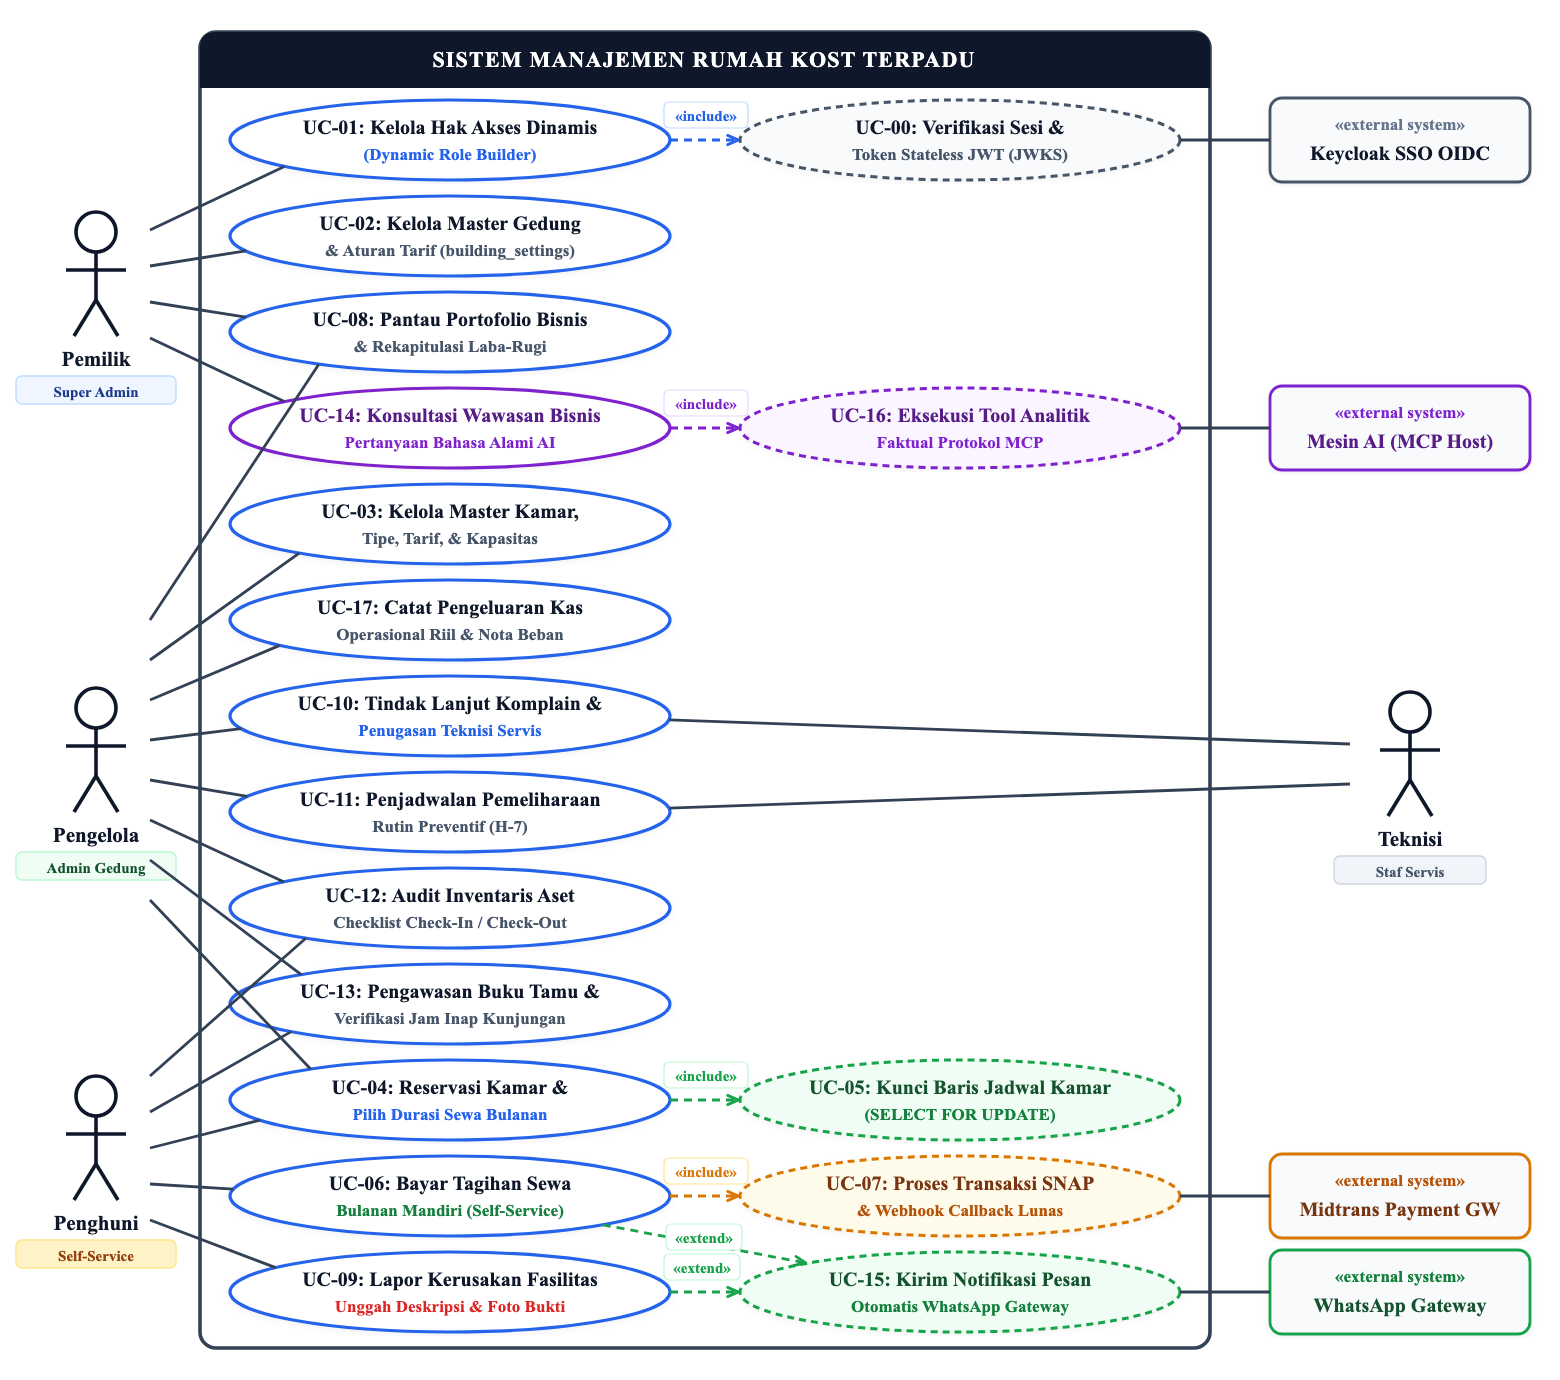
\includegraphics[width=0.92\textwidth,height=0.72\textheight,keepaspectratio]{assets/diagrams/bab3_14_use_case_global.png}
  \caption{Use Case Diagram Sistem Manajemen Rumah Kost}
  \label{fig:use_case}
\end{figure}

Deskripsi hubungan penggunaan (\textit{use case}) pada Gambar~\ref{fig:use_case} dirangkum ke dalam lima kelompok fungsi utama pada Tabel~\ref{tab:use_case}.

\begin{table}[H]
  \centering
  \caption{Ringkasan Spesifikasi Use Case Sistem}
  \label{tab:use_case}
  \begin{tblr}{
    width = \textwidth,
    colspec = {Q[c,1.3cm] X[1.6,l] X[1.2,l] X[1.3,l] X[2.3,l]}
  }
    ID & Nama Use Case & Aktor Utama & Modul Domain & Lingkup Aksi Utama \\
    UC-01 & Pengelolaan Gedung dan Kamar & Pemilik, Pengelola & Building, Room & Registrasi gedung baru, pengaturan \texttt{min\_rental\_months}, penambahan unit kamar, dan pengubahan status fisik unit. \\
    UC-02 & Reservasi Kamar dan Pembayaran Digital & Penghuni & Lease, Finance & Pemilihan unit kamar, penguncian baris jadwal anti-bentrok, penerbitan tagihan otomatis, dan transaksi via Midtrans SNAP. \\
    UC-03 & Pengajuan dan Penanganan Tiket Kerusakan & Penghuni, Pengelola, Teknisi & Maintenance, Room & Unggah foto keluhan kerusakan, isolasi status kamar jika fatal, penugasan teknisi, dan konfirmasi perbaikan selesai. \\
    UC-04 & Konsultasi Wawasan Bisnis berbasis AI & Pemilik, Pengelola & MCP, Module Gateway & Eksekusi pemanggilan perkakas baca analitik (okupansi, kas masuk, piutang, dan tiket) secara deterministik tanpa halusinasi. \\
    UC-05 & Inventarisasi Aset dan Buku Tamu & Pengelola, Penghuni & Inventory, Guest & Checklist fisik perabot kamar saat serah terima huni, pencatatan jam tamu masuk/keluar, dan pembebanan biaya inap. \\
  \end{tblr}
\end{table}

\subsection{Data Flow Diagram (DFD Level 0 dan Level 1)}
\label{sec:dfd}

\textit{Data Flow Diagram} (DFD) memodelkan aliran pertukaran data secara terstruktur, mulai dari sumber data eksternal (\textit{terminator}), tahapan proses komputasi di dalam sistem, hingga penyimpanan data (\textit{data store}) yang terisolasi. Pemodelan DFD disusun mengikuti standar DeMarco dan Yourdon, yang membagi aliran data ke dalam dua tingkatan: Diagram Konteks (Level 0) dan Diagram Dekomposisi Fungsional (Level 1).

\subsubsection{DFD Level 0 (Diagram Konteks)}

Diagram Konteks mendefinisikan batas sistem (\textit{system boundary}) secara menyeluruh. Seluruh fungsionalitas aplikasi diwakili oleh satu lingkaran proses utama (Proses 0.0) yang berinteraksi dengan tujuh entitas luar tanpa menampilkan komponen penyimpanan data internal, seperti diperlihatkan pada Gambar~\ref{fig:dfd_l0}.

\begin{figure}[H]
  \centering
  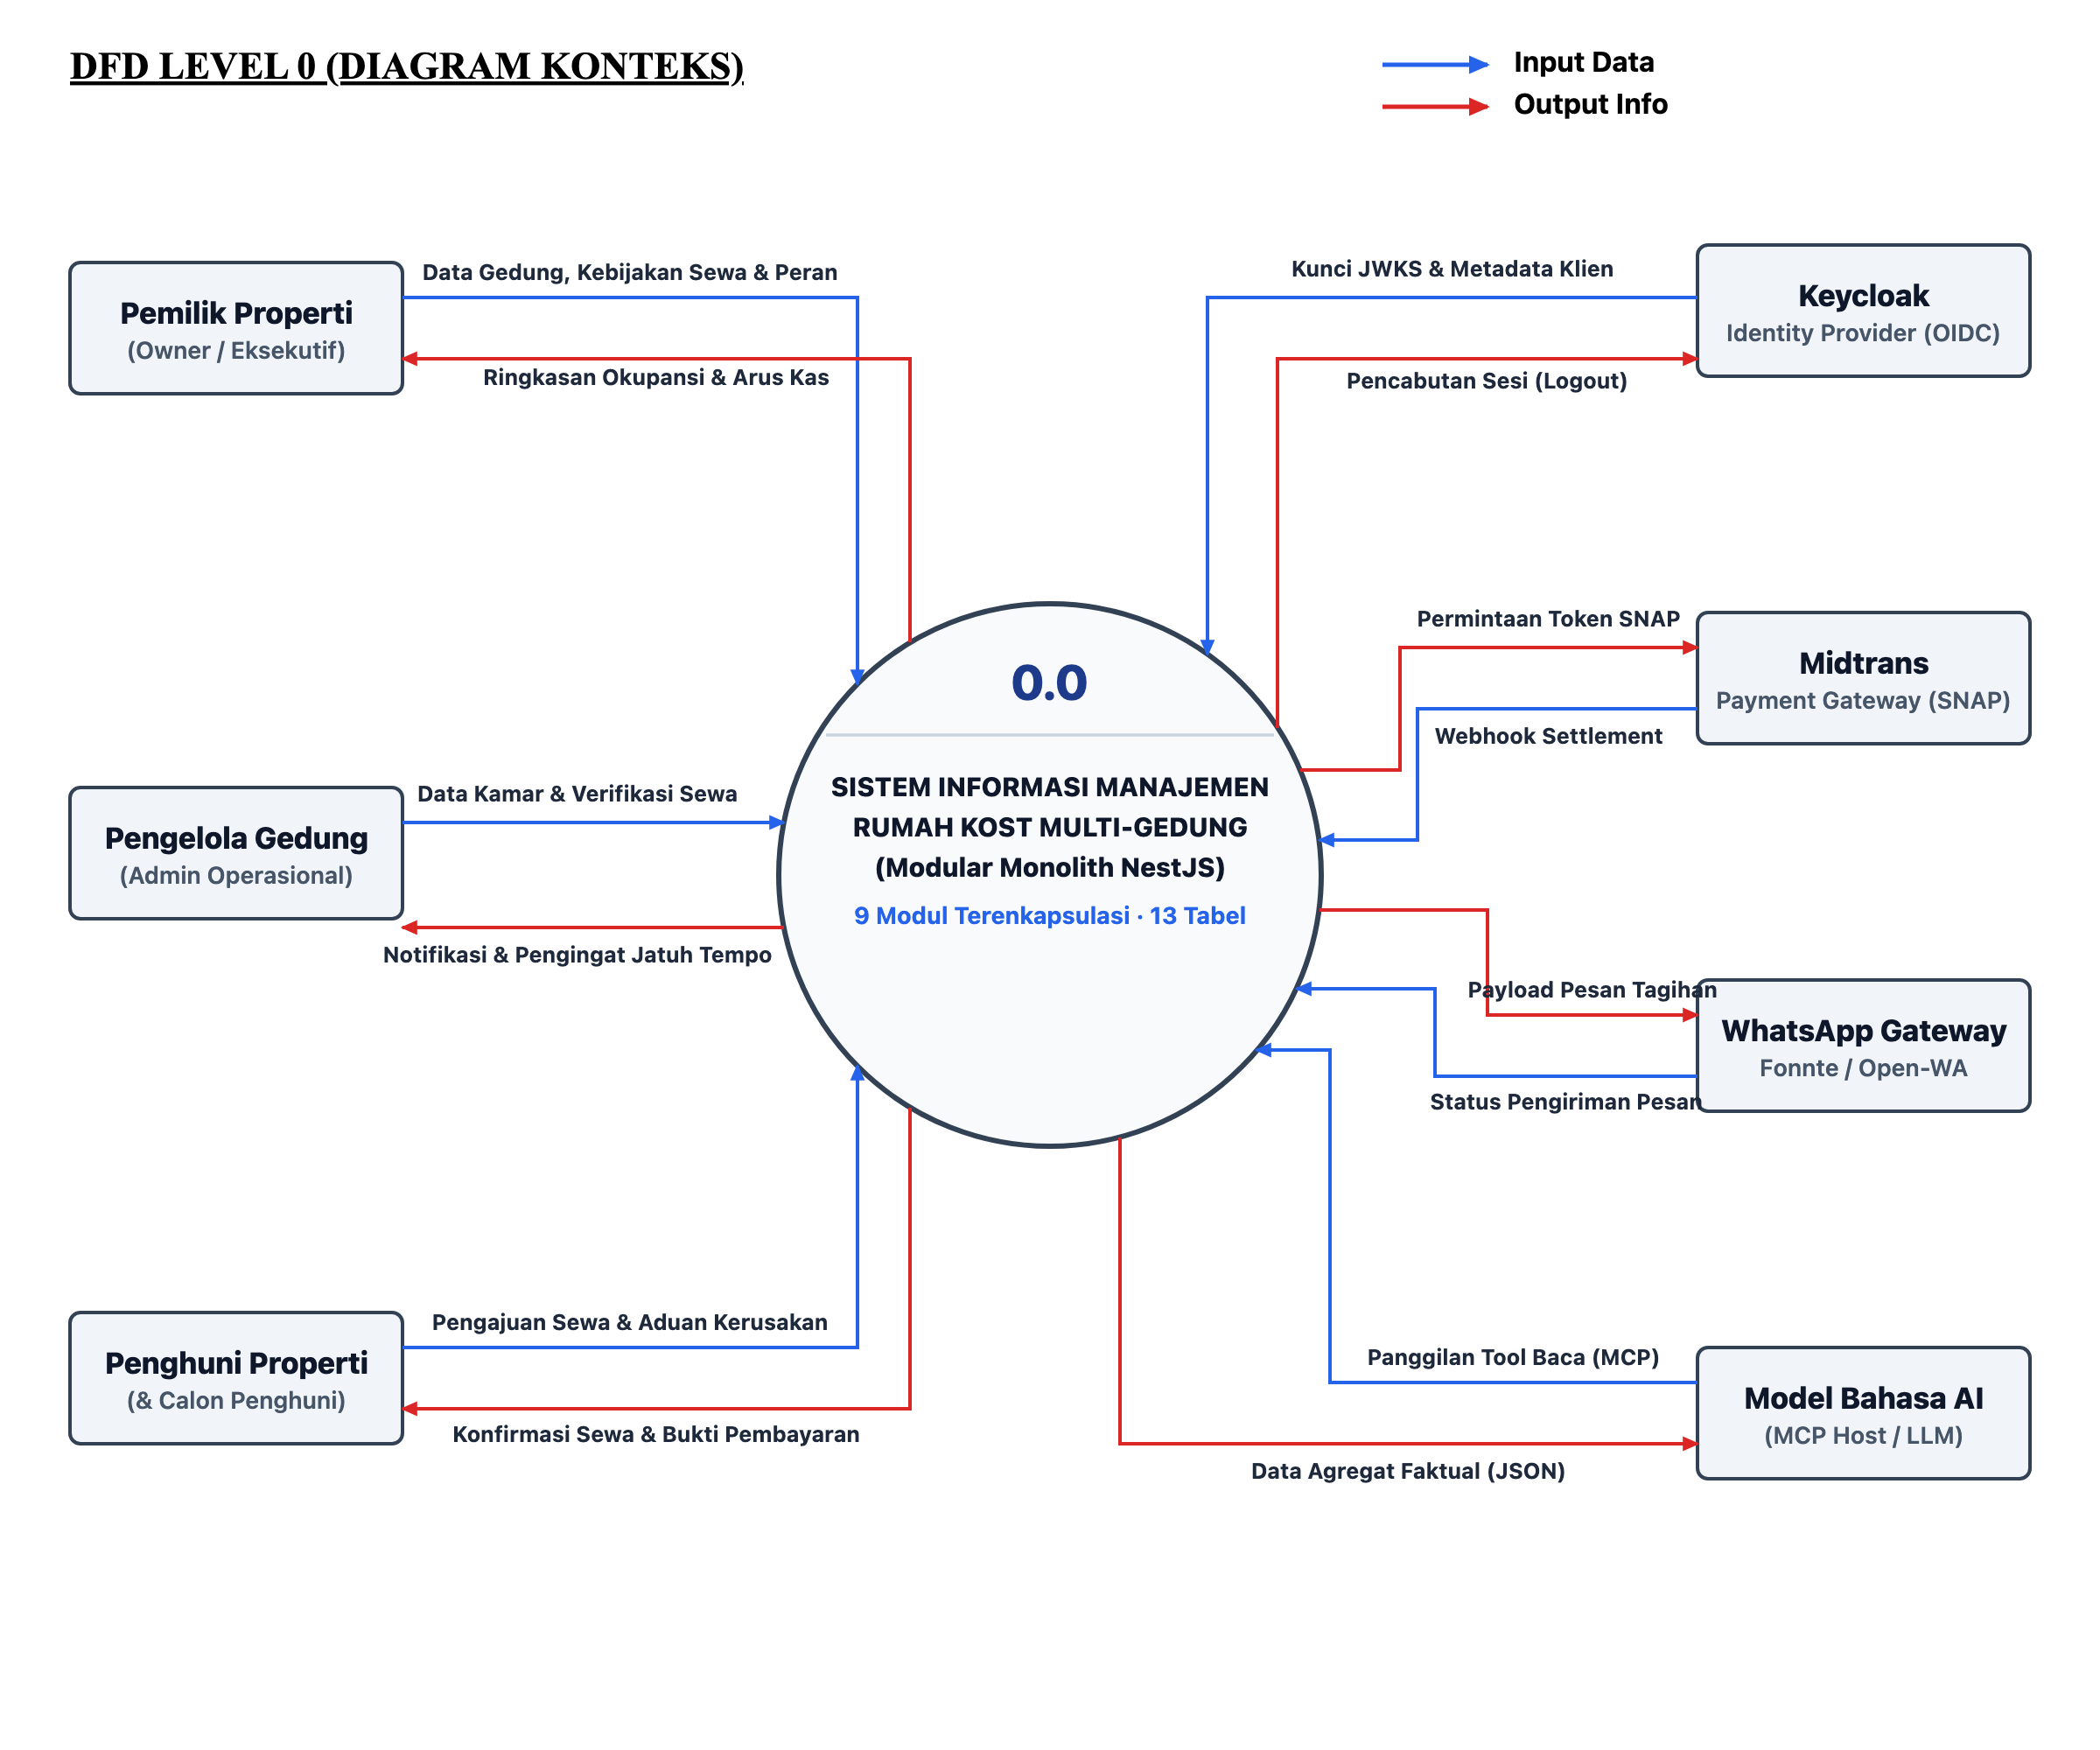
\includegraphics[width=0.95\textwidth,height=0.72\textheight,keepaspectratio]{assets/diagrams/bab3_15_dfd_level_0.png}
  \caption{Data Flow Diagram (DFD) Level 0 / Diagram Konteks}
  \label{fig:dfd_l0}
\end{figure}

Berdasarkan Gambar~\ref{fig:dfd_l0}, pertukaran data antara Proses 0.0 dengan ketujuh entitas luar meliputi:
\begin{enumerate}[label=\arabic*., leftmargin=*]
  \item \textbf{Pemilik Properti (\textit{Owner}):} Mengirimkan data input berupa registrasi akun, pendaftaran gedung baru, pengaturan tarif dan durasi sewa, serta konfigurasi izin peran kustom. Sistem mengembalikan data keluaran berupa dasbor okupansi seluruh gedung, laporan laba rugi kas riil, dan rekapitulasi audit pengguna.
  \item \textbf{Pengelola Gedung (\textit{Admin}):} Memasukkan data unit kamar, penugasan teknisi tiket komplain, pencatatan nota kas keluar operasional, checklist kondisi aset kamar, dan konfirmasi kedatangan tamu. Sistem memberikan data keluaran berupa daftar kamar gedung binaan, tiket komplain masuk, jadwal jatuh tempo servis fasilitas H-7, serta rekapitulasi buku tamu aktif.
  \item \textbf{Penghuni (\textit{Resident}):} Memasukkan data permohonan reservasi kamar, konfirmasi pembayaran tagihan, tiket aduan kerusakan fasilitas berfoto, dan pra-registrasi identitas tamu. Sistem memberikan konfirmasi penempatan sewa, lembar invoice tagihan, tautan pembayaran online, serta notifikasi progres penanganan perbaikan.
  \item \textbf{Keycloak (Identity Provider OIDC):} Menerima kredensial masuk dari pengguna dan mengembalikan token akses JWT yang memuat klaim peran serta batasan properti.
  \item \textbf{Midtrans (Payment Gateway):} Menerima permintaan token transaksi SNAP (nomor order dan nominal tagihan), lalu mengirimkan notifikasi \textit{webhook callback} mengenai status penyelesaian pembayaran secara \textit{real-time}.
  \item \textbf{WhatsApp Gateway:} Menerima muatan pesan teks otomatis (rincian invoice, pengingat jatuh tempo, kuitansi pelunasan) beserta nomor telepon tujuan, dan mengembalikan status konfirmasi pengiriman pesan.
  \item \textbf{Model Bahasa AI (MCP Host / LLM):} Mengirimkan perintah pemanggilan perkakas analitik berbasis format JSON-RPC 2.0 dan menerima hasil ekstraksi data faktual JSON yang teragregasi secara aman.
\end{enumerate}

\subsubsection{DFD Level 1 (Dekomposisi Fungsional)}

DFD Level 1 mendekomposisi Proses 0.0 menjadi sepuluh proses fungsional mandiri yang mencerminkan pembagian sepuluh modul backend NestJS (sembilan modul bisnis ditambah satu Modul \texttt{AI / MCP Assistant}). Masing-masing proses bertanggung jawab penuh atas penyimpanan data (\textit{data store}) yang dimilikinya, sebagaimana disajikan pada Gambar~\ref{fig:dfd_l1}.

\begin{figure}[H]
  \centering
  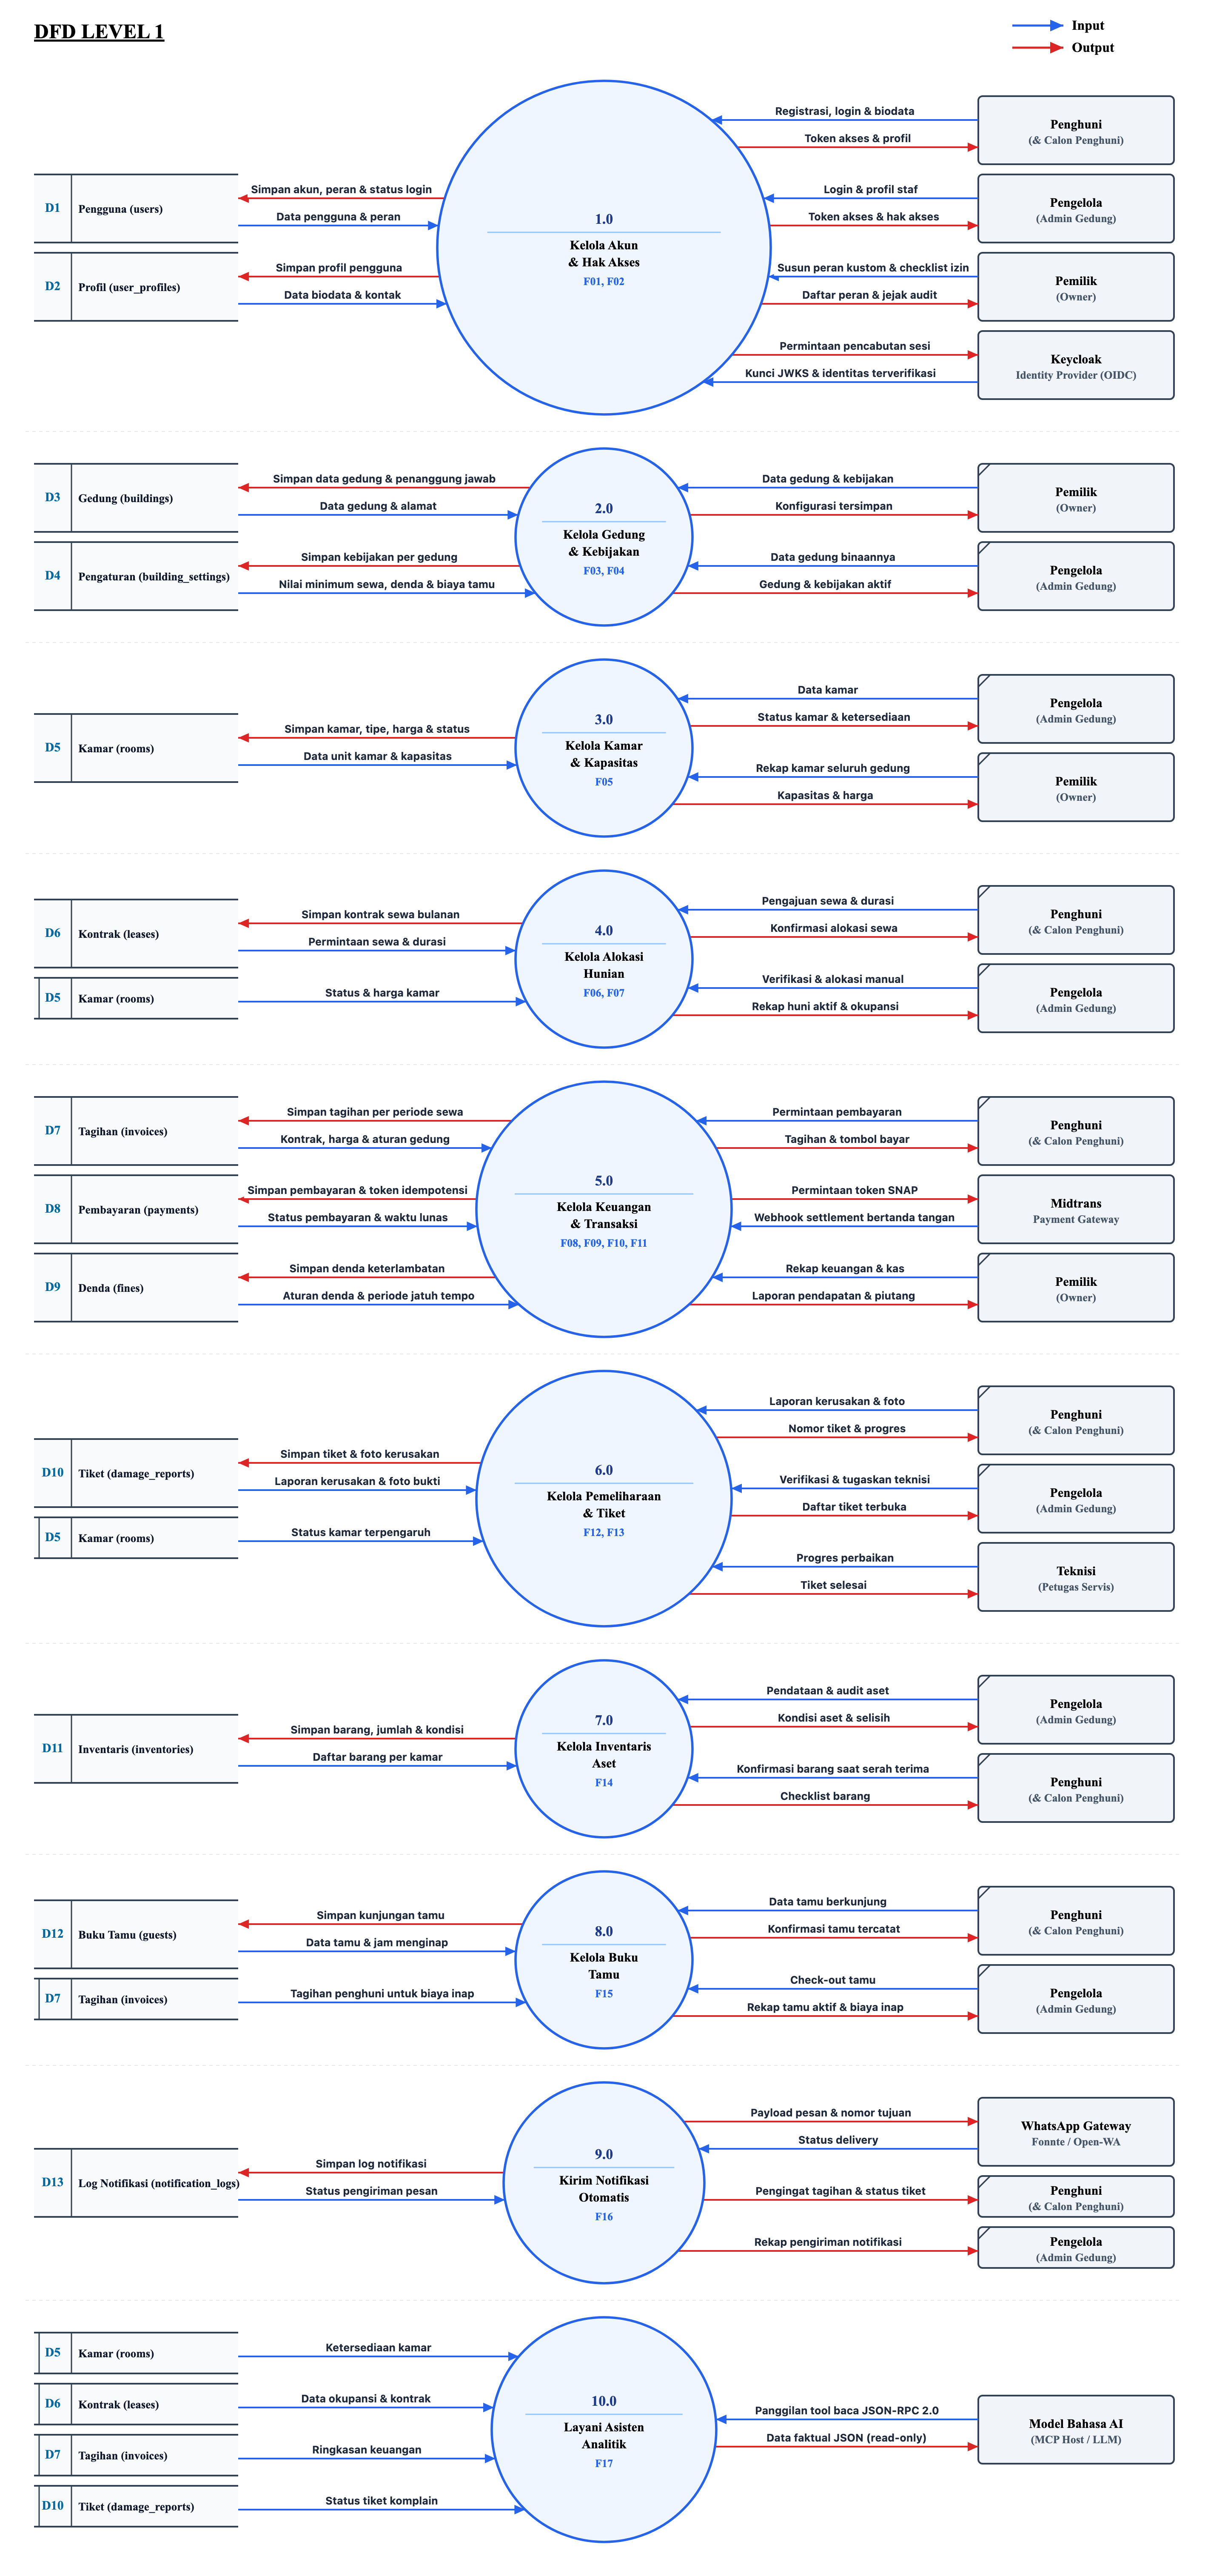
\includegraphics[width=0.95\textwidth,height=0.78\textheight,keepaspectratio]{assets/diagrams/bab3_16_dfd_level_1.png}
  \caption{Data Flow Diagram (DFD) Level 1}
  \label{fig:dfd_l1}
\end{figure}

Sepuluh proses fungsional beserta keterkaitannya dengan 13 \textit{data store} (D1 sampai D13) dijelaskan pada Tabel~\ref{tab:dfd_l1}.

\begin{longtblr}[
  caption = {Pemetaan Proses Fungsional, Fitur, dan Data Store pada DFD Level 1},
  label = {tab:dfd_l1}
]{
  width = \textwidth,
  colspec = {Q[c,1.1cm] X[1.4,l] Q[c,1.4cm] X[1.8,l] X[2.3,l]}
}
  No. Proses & Nama Proses Fungsional & Fitur Terkait & Data Store yang Dikelola & Keterangan Aliran Data \\
  1.0 & Kelola Akun dan Hak Akses & F01, F02 & D1 \texttt{users}, D2 \texttt{user\_profiles} & Menyimpan kredensial akun, mengikat peran Keycloak, dan mengelola biodata pengguna. \\
  2.0 & Kelola Gedung dan Kebijakan & F03, F04 & D3 \texttt{buildings}, D4 \texttt{building\_settings} & Menyimpan profil fisik gedung dan konfigurasi parameter operasional (durasi minimal sewa, tarif denda, toleransi tamu). \\
  3.0 & Kelola Kamar dan Kapasitas & F05 & D5 \texttt{rooms} & Mengelola data kamar, tipe, dan harga bulanan. Menerima instruksi penguncian status kamar dari proses pemeliharaan. \\
  4.0 & Kelola Alokasi Hunian & F06, F07 & D6 \texttt{leases} (membaca D4 dan D5) & Memvalidasi durasi sewa terhadap aturan gedung, mengunci kamar, menyimpan kontrak aktif, dan menyajikan dasbor okupansi. \\
  5.0 & Kelola Keuangan dan Transaksi & F08, F09, F10, F11 & D7 \texttt{invoices}, D8 \texttt{payments}, D9 \texttt{fines} & Menerbitkan tagihan sewa, memproses token SNAP Midtrans, mencatat pembayaran manual/digital, dan menghitung laba bersih operasional. \\
  6.0 & Kelola Pemeliharaan dan Tiket & F12, F13 & D10 \texttt{damage\_reports} (memperbarui D5) & Menerima komplain kerusakan berlampiran foto dari penghuni, menugaskan teknisi, dan menjadwalkan servis rutin preventif. \\
  7.0 & Kelola Inventaris Aset & F14 & D11 \texttt{inventories} (membaca D5) & Mencatat daftar inventaris perabot unit kamar dan menyimpan hasil verifikasi checklist fisik saat serah terima. \\
  8.0 & Kelola Buku Tamu & F15 & D12 \texttt{guests} (meneruskan biaya ke D7) & Mencatat log kunjungan tamu dan meneruskan biaya inap tambahan ke modul keuangan jika tamu melewati batas jam malam. \\
  9.0 & Kirim Notifikasi Otomatis & F16 & D13 \texttt{notification\_logs} & Menangkap kejadian transaksi dari \textit{event bus} dan mengirim pesan pengingat tagihan/kuitansi ke WhatsApp Gateway. \\
  10.0 & Layani Asisten Analitik & F17 & Operasi baca murni dari D5, D6, D7, dan D10 & Mengagregasi data statistik ketersediaan kamar, keuangan, dan tiket kerusakan untuk disajikan kembali ke antarmuka AI. \\
\end{longtblr}

Aturan isolasi data ditegakkan secara ketat pada DFD Level 1: tidak ada proses yang diperkenankan menulis (\textit{write}) langsung ke \textit{data store} milik proses lain. Seluruh koordinasi lintas proses dilakukan secara asinkron melalui pertukaran kejadian domain (\textit{event bus}) atau secara sinkron melalui antarmuka \textit{Module Gateway}.

\section{RANCANGAN BASIS DATA}
\label{sec:basis_data}

Sistem menggunakan sistem manajemen basis data relasional (\textit{Relational Database Management System} / RDBMS) PostgreSQL. Seluruh modul backend berbagi satu basis data bersama (\textit{shared database}). Isolasi data antar-gedung ditegakkan di level baris (\textit{row-level scoping}) menggunakan kolom penanda \texttt{building\_id}, sehingga seluruh kueri operasional terisolasi per properti secara aman dan efisien.

\subsection{Entity Relationship Diagram}
\label{subsec:erd}

Rancangan basis data baru (\textit{after}) ini merupakan hasil penyederhanaan dan \textit{refactoring} menyeluruh terhadap ERD sistem sebelum \textit{rewrite} pada Subbab~\ref{subsec:evolusi_desain} (lihat Gambar~\ref{fig:erd_lama} di Bab~II) yang sebelumnya membengkak hingga 34 tabel domain akibat percabangan masa sewa dan duplikasi tabel penampung. Pada sistem baru ini, model data dirancang dengan menegakkan batas modul (\textit{modular boundaries}) melalui penyederhanaan aturan sewa menjadi bulanan murni dan penerapan pola \textit{Two-Phase Invoicing}. Untuk menjaga agar modul backend tetap independen dan tidak saling terikat kaku di level skema fisik seperti pada sistem lama, ketergantungan relasi \textit{Foreign Key} (FK) fisik hanya diizinkan di dalam modul yang sama (intra-modul). Hubungan lintas domain dikelola sepenuhnya melalui referensi logis (\textit{soft reference}) yang diperkuat oleh indeks kolom dan penyaringan \texttt{building\_id}, sebagaimana ditunjukkan pada Gambar~\ref{fig:erd_baru}.

\begin{figure}[H]
  \centering
  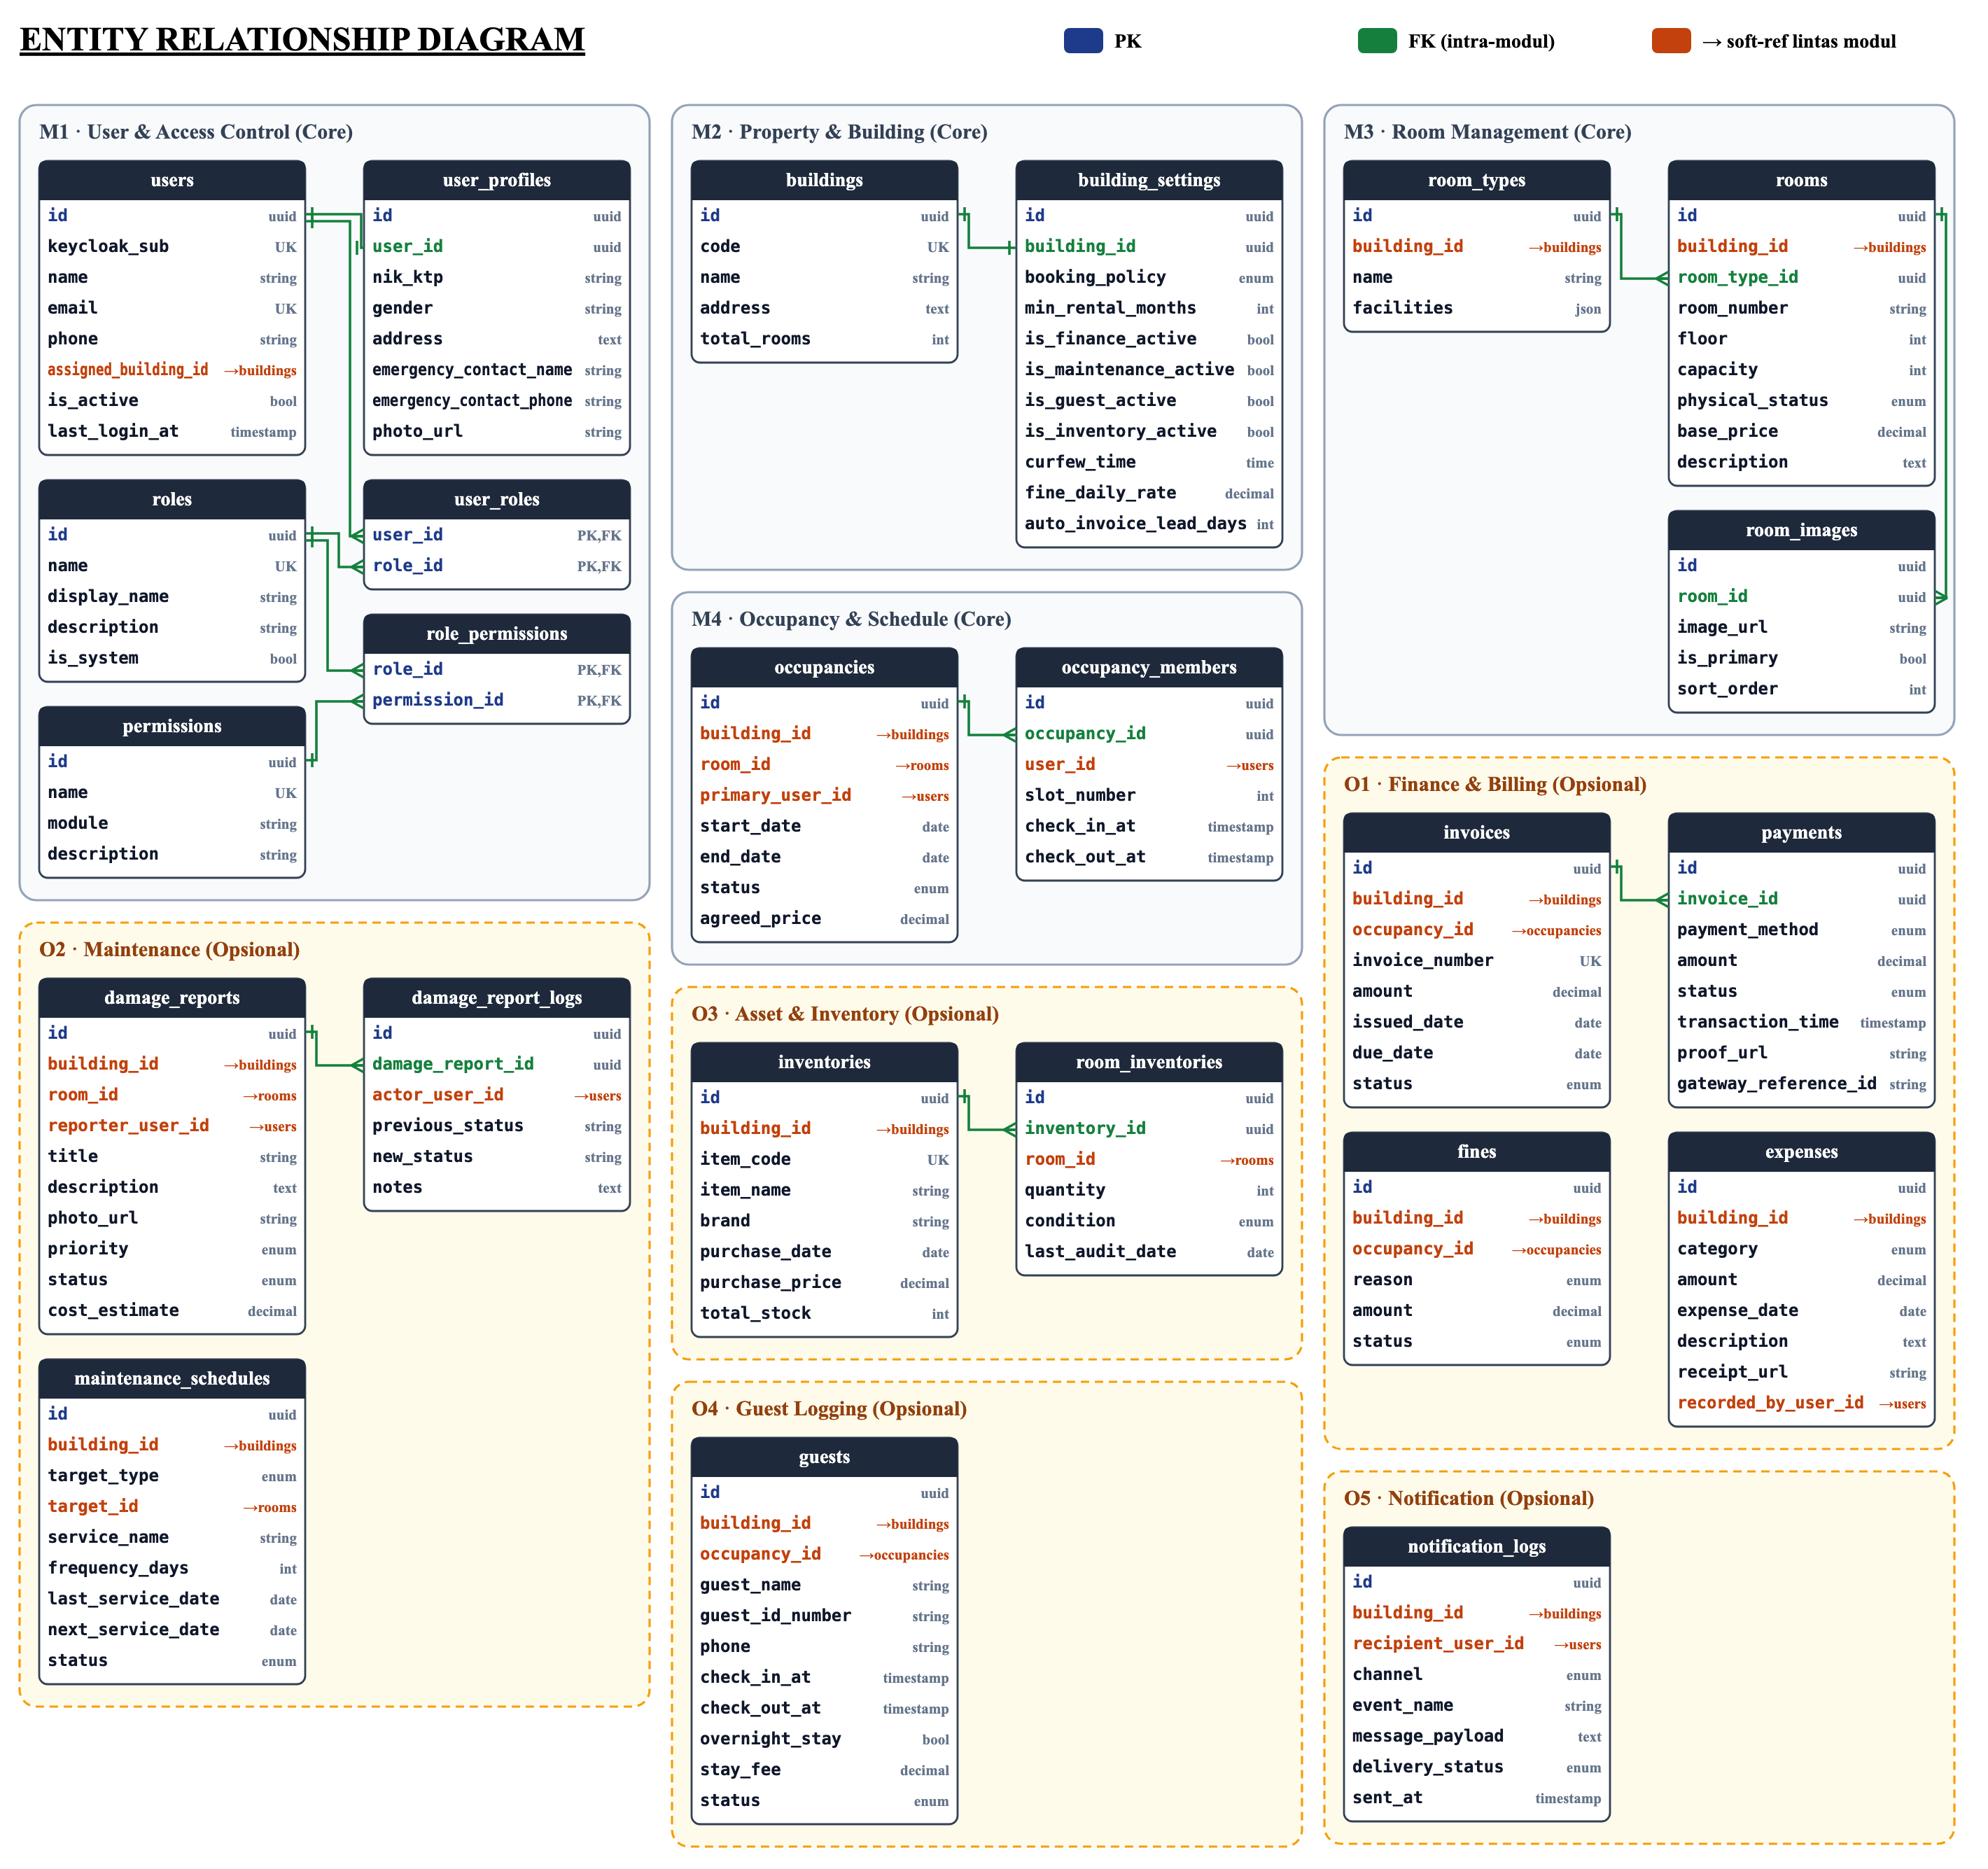
\includegraphics[width=0.98\textwidth,height=0.76\textheight,keepaspectratio]{assets/diagrams/bab3_17_erd_sistem_dinamis.png}
  \caption{Entity Relationship Diagram}
  \label{fig:erd_baru}
\end{figure}

Gambar~\ref{fig:erd_baru} mengelompokkan 21 tabel domain utama ke dalam sembilan modul pemilik data, sedangkan modul kesepuluh (\texttt{O6 --- AI / MCP Assistant}) beroperasi secara \textit{stateless} dan \textit{read-only} melalui \textit{Module Gateway} tanpa menambah tabel transaksi bisnis baru:
\begin{enumerate}[label=\arabic*., leftmargin=*]
  \item \textbf{M1 --- User \& Access Control (Core):}
    \begin{enumerate}[label=\alph*., leftmargin=*]
      \item \texttt{users}: Identitas utama pengguna yang terhubung ke Keycloak (\texttt{keycloak\_sub}), surel, nama, status aktif, dan batas gedung bawaan (\texttt{assigned\_building\_id}).
      \item \texttt{user\_profiles}: Profil biodata pengguna mencakup NIK KTP, jenis kelamin, alamat, nomor darurat, dan foto identitas (relasi \textit{1-to-1} dengan \texttt{users}).
      \item \texttt{roles}, \texttt{permissions}, \texttt{user\_roles}, \texttt{role\_permissions}: Pengaturan peran kustom dan hak akses granular berbasis sistem RBAC dinamis.
    \end{enumerate}
  \item \textbf{M2 --- Property \& Building (Core):}
    \begin{enumerate}[label=\alph*., leftmargin=*]
      \item \texttt{buildings}: Master data fisik gedung properti (kode unik, nama, alamat, total unit kamar).
      \item \texttt{building\_settings}: Konfigurasi kebijakan per gedung seperti kebijakan pemesanan (\texttt{booking\_policy}), durasi sewa minimal (\texttt{min\_rental\_months}), sakelar fitur modul opsional, jam malam, dan tarif denda.
    \end{enumerate}
  \item \textbf{M3 --- Room Management (Core):}
    \begin{enumerate}[label=\alph*., leftmargin=*]
      \item \texttt{room\_types}: Tipe/kategori kamar beserta daftar fasilitas pendukung dalam format JSON.
      \item \texttt{rooms}: Unit fisik kamar mencakup nomor unit, lantai, kapasitas, tarif dasar bulanan, dan status fisik (\texttt{physical\_status}).
      \item \texttt{room\_images}: Galeri foto unit kamar beserta urutan tampilan dan penanda foto utama.
    \end{enumerate}
  \item \textbf{M4 --- Occupancy \& Schedule (Core):}
    \begin{enumerate}[label=\alph*., leftmargin=*]
      \item \texttt{occupancies}: Transaksi kontrak huni dan alokasi sewa bulanan, mencakup penghuni utama, rentang tanggal sewa, kesepakatan harga, serta status kontrak.
      \item \texttt{occupancy\_members}: Daftar anggota/penghuni tambahan yang menempati unit kamar terkait beserta riwayat \textit{check-in}/\textit{check-out}.
    \end{enumerate}
  \item \textbf{O1 --- Finance \& Billing (Opsional):}
    \begin{enumerate}[label=\alph*., leftmargin=*]
      \item \texttt{invoices}: Lembar tagihan sewa berkala per periode sewa beserta status pembayaran dan tenggat jatuh tempo.
      \item \texttt{payments}: Catatan transaksi pembayaran digital (Midtrans SNAP) atau kasir manual berlampiran bukti transfer.
      \item \texttt{fines}: Catatan denda keterlambatan pembayaran tagihan.
      \item \texttt{expenses}: Catatan pengeluaran kas operasional gedung berlampiran foto nota bukti pengeluaran.
    \end{enumerate}
  \item \textbf{O2 --- Maintenance (Opsional):}
    \begin{enumerate}[label=\alph*., leftmargin=*]
      \item \texttt{damage\_reports} \& \texttt{damage\_report\_logs}: Tiket laporan kerusakan fasilitas dari penghuni berlampiran foto serta rekam jejak perubahan status perbaikan.
      \item \texttt{maintenance\_schedules}: Agenda pemeliharaan rutin preventif untuk fasilitas gedung.
    \end{enumerate}
  \item \textbf{O3 --- Asset \& Inventory (Opsional):}
    \begin{enumerate}[label=\alph*., leftmargin=*]
      \item \texttt{inventories} \& \texttt{room\_inventories}: Master data inventaris aset gedung serta pemetaan perabot per kamar beserta kondisi dan tanggal audit terakhir.
    \end{enumerate}
  \item \textbf{O4 --- Guest Logging (Opsional):}
    \begin{enumerate}[label=\alph*., leftmargin=*]
      \item \texttt{guests}: Buku tamu digital untuk mencatat riwayat kunjungan, jam masuk/keluar, status menginap, dan pembebanan biaya inap tambahan.
    \end{enumerate}
  \item \textbf{O5 --- Notification (Opsional):}
    \begin{enumerate}[label=\alph*., leftmargin=*]
      \item \texttt{notification\_logs}: Log riwayat pengiriman notifikasi otomatis (WhatsApp/Email) mencakup nama event, muatan pesan, dan status pengiriman.
    \end{enumerate}
  \item \textbf{O6 --- AI / MCP Assistant (Opsional):}
    \begin{enumerate}[label=\alph*., leftmargin=*]
      \item Tidak memiliki tabel transaksi tersendiri; seluruh kebutuhan kueri analitik dibaca secara \textit{stateless} dan \textit{read-only} melalui \textit{Query Gateway} dengan penyaringan klaim \texttt{building\_id}.
    \end{enumerate}
\end{enumerate}

\section{RANCANGAN EVALUASI SISTEM}
\label{sec:rancangan_evaluasi}

Evaluasi sistem dirancang untuk memverifikasi ketercapaian seluruh rumusan masalah dan tujuan pada Bab~I secara terukur dan objektif tanpa bergantung pada penilaian subjektif. Pengujian berfokus pada keandalan fungsional, isolasi modularitas sepuluh modul, isolasi data antar-\textit{tenant}, idempotensi pembayaran digital, serta akurasi dan keamanan \textit{read-only} Modul AI.

\subsection{Alur Evaluasi Sistem (\textit{Flowchart} Evaluasi)}

Tahapan pelaksanaan evaluasi sistem dari persiapan lingkungan uji hingga penarikan kesimpulan hasil dimodelkan pada Gambar~\ref{fig:flowchart_evaluasi}.

\begin{figure}[H]
  \centering
  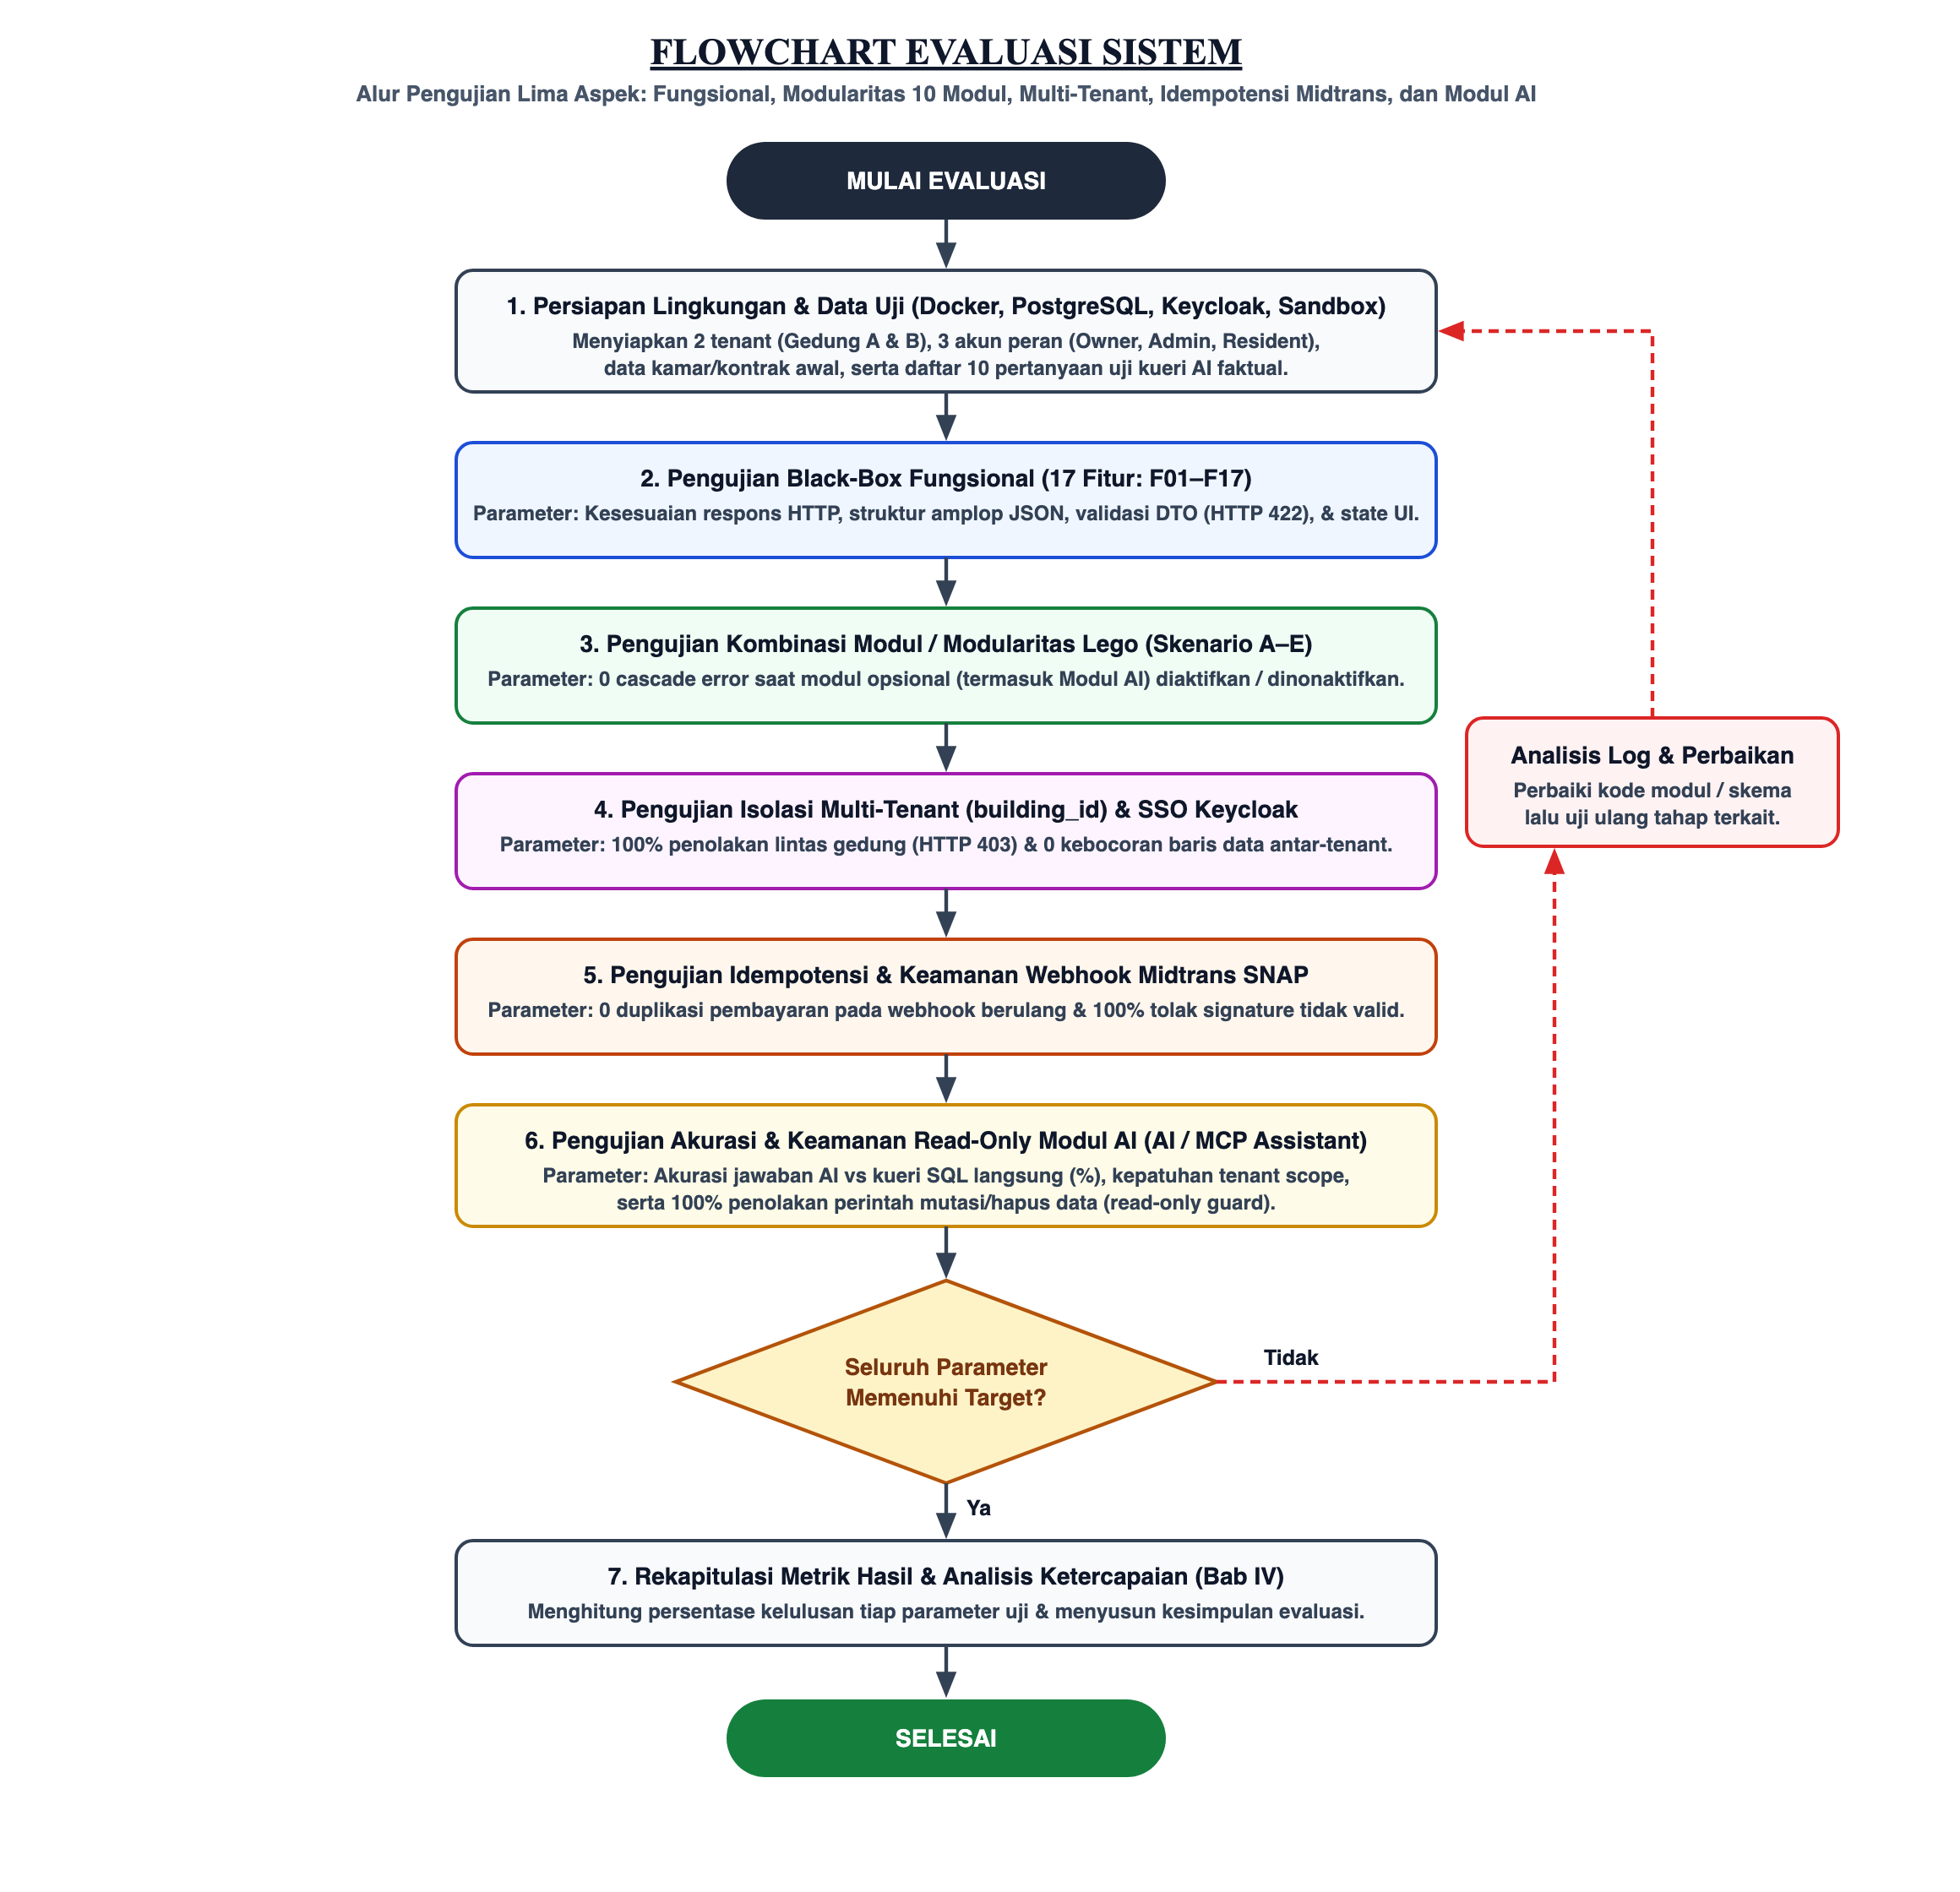
\includegraphics[width=0.92\textwidth,height=0.78\textheight,keepaspectratio]{assets/diagrams/bab3_18_flowchart_evaluasi.png}
  \caption{Flowchart Evaluasi Sistem}
  \label{fig:flowchart_evaluasi}
\end{figure}

Berdasarkan Gambar~\ref{fig:flowchart_evaluasi}, evaluasi dijalankan secara berurutan dimulai dari penyediaan dua gedung uji (Gedung~A dan Gedung~B) beserta tiga akun peran (\textit{Owner}, \textit{Admin}, dan \textit{Resident}) pada lingkungan kontainer Docker, dilanjutkan dengan eksekusi lima tahap pengujian teknis. Apabila ditemukan parameter yang belum memenuhi target keberhasilan, dilakukan analisis log dan perbaikan kode sebelum tahap pengujian terkait diulang kembali.

\subsection{Parameter, Cara Pengujian, dan Skenario Uji}

Rincian parameter yang diukur, cara pelaksanaan pengujian, instrumen yang digunakan, dan target keberhasilan untuk kelima aspek evaluasi dirangkum pada Tabel~\ref{tab:parameter_evaluasi}.

\begin{longtblr}[
  caption = {Rancangan Parameter dan Metode Evaluasi Sistem},
  label = {tab:parameter_evaluasi}
]{
  width = \textwidth,
  colspec = {Q[c,0.7cm] X[1.3,l] X[1.6,l] X[1.9,l] X[1.4,l]}
}
  No & Aspek Evaluasi & Parameter yang Diukur & Cara Melakukan Pengujian & Kriteria Keberhasilan \\
  1 & Pengujian \textit{Black-Box} Fungsional (17 Fitur) & Kesesuaian kode status HTTP, struktur amplop JSON, validasi DTO (HTTP 422), dan perubahan \textit{state} antarmuka. & Menjalankan skenario input valid dan tidak valid untuk seluruh fitur \texttt{F01}--\texttt{F17} melalui dokumentasi Swagger/HTTP \textit{client} serta antarmuka Flutter Web. & 100\% skenario uji fungsional berjalan sesuai spesifikasi tanpa galat server (HTTP 500). \\
  2 & Pengujian Kombinasi Modul (Modularitas) & Jumlah galat dependensi atau \textit{cascade error} saat modul opsional diaktifkan/dinonaktifkan. & Menjalankan alur inti penyewaan kamar pada lima kombinasi sakelar modul (Skenario A--E pada Tabel~\ref{tab:pengujian_lego}) dengan mengaktifkan dan menonaktifkan modul opsional. & 0 \textit{cascade error}; seluruh alur inti tetap berjalan normal pada semua kombinasi. \\
  3 & Pengujian Isolasi \textit{Multi-Tenant} (\texttt{building\_id}) & Tingkat penolakan akses lintas gedung dan jumlah baris data bocor antar-\textit{tenant}. & Mengirim permintaan baca dan tulis ke sumber daya Gedung~B menggunakan token JWT \textit{Admin} atau \textit{Resident} yang terikat pada Gedung~A. & 100\% permintaan lintas gedung ditolak (HTTP 403) dan 0 baris data Gedung~B tampil. \\
  4 & Pengujian Idempotensi \textit{Webhook} Midtrans & Konsistensi status tagihan/pembayaran dan penolakan tanda tangan tidak valid. & Mengirim ulang \textit{payload webhook} Midtrans identik sebanyak $\ge 3$ kali berurutan (simulasi \textit{retry}), serta mengirim \textit{webhook} dengan \textit{signature\_key} palsu. & 0 duplikasi catatan pembayaran dan 100\% \textit{webhook} palsu ditolak. \\
  5 & Pengujian Akurasi \& Keamanan Modul AI (\texttt{AI / MCP Assistant}) & Akurasi jawaban faktual (\%), kepatuhan \textit{tenant scope}, dan penolakan perintah tulis/hapus. & Menguji minimal 10 pertanyaan manajerial (okupansi, tunggakan, komplain, kas) lalu membandingkan angka jawaban AI dengan hasil kueri SQL langsung PostgreSQL, serta menguji permintaan mutasi data. & Akurasi data faktual 100\% sesuai basis data dan 100\% perintah tulis/hapus ditolak (\textit{read-only guard}). \\
\end{longtblr}

Khusus untuk aspek evaluasi kedua (modularitas), sistem dirancang untuk diuji melalui lima skenario kombinasi modul pada gedung yang berbeda, termasuk skenario pengujian dengan Modul \texttt{AI / MCP Assistant} aktif maupun nonaktif, sebagaimana tercantum pada Tabel~\ref{tab:pengujian_lego}.

\begin{table}[H]
  \centering
  \caption{Rancangan Skenario Pengujian Kombinasi Modul Lego}
  \label{tab:pengujian_lego}
  \begin{tblr}{
    width = \textwidth,
    colspec = {Q[c,1.9cm] X[1.9,l] X[1.5,l] X[2.2,l]}
  }
    Skenario & Kombinasi Modul Aktif & Modul Dinonaktifkan & Target Verifikasi Integrasi \\
    Skenario A & Core + Finance + Maintenance + Inventory + Guest + Notification + AI/MCP & Tidak Ada (Penuh) & Seluruh alur transaksi, tiket, audit, WhatsApp, dan konsultasi AI berjalan tanpa konflik batas modul. \\
    Skenario B & Core + Maintenance + Inventory + Guest + AI/MCP & Finance, Notification & Kontrak huni dikonfirmasi otomatis tanpa invoice, sementara AI tetap menjawab kueri okupansi dan tiket. \\
    Skenario C & Core + Finance + Notification & Maintenance, Inventory, Guest, AI/MCP & Sistem berfokus pada sewa dan transaksi keuangan tanpa menu operasional lapangan maupun layanan AI. \\
    Skenario D & Core + AI/MCP & Finance, Maintenance, Inventory, Guest, Notification & Sistem pencatatan kamar dan kontrak inti berjalan berdampingan dengan Modul AI khusus kueri hunian. \\
    Skenario E & Core Saja (Auth, Building, Room, Lease) & Seluruh Modul Opsional & Sistem berfungsi murni sebagai pencatatan master kamar dan alokasi hunian tanpa modul tambahan. \\
  \end{tblr}
\end{table}

\section{TIMELINE PENGERJAAN}
\label{sec:timeline_pengerjaan}

Rencana pelaksanaan pengerjaan Proyek Akhir dijadwalkan secara terstruktur mengikuti tahapan rancangan penelitian dan empat siklus \textit{sprint} Scrum, sebagaimana disajikan pada Tabel~\ref{tab:timeline}.

\begin{table}[H]
  \centering
  \caption{Timeline Pengerjaan Proyek Akhir}
  \label{tab:timeline}
  \begin{tblr}{
    width = \textwidth,
    colspec = {Q[c,0.7cm] X[2.3,l] X[1.4,l] X[2.2,l]}
  }
    No & Tahap / Aktivitas Utama & Periode & Luaran Utama \\
    1 & Analisis Masalah, Studi Literatur, dan Audit Sistem Lama & Bulan ke-1 (Minggu 1--4) & Pemetaan 8 kelemahan sistem lama dan skema 34 tabel terdahulu. \\
    2 & Perancangan Arsitektur \textit{Modular Monolith}, BPMN, DFD, dan ERD & Bulan ke-2 (Minggu 1--4) & Dokumen desain 10 modul, 9 BPMN, DFD L0--L1, dan ERD 21 tabel. \\
    3 & Implementasi \textit{Sprint 1}: Docker, PostgreSQL, Keycloak SSO, dan 4 Modul \textit{Core} & Bulan ke-3 (Minggu 1--2) & Autentikasi OIDC, \textit{multi-tenant scoping}, dan alur sewa inti berjalan. \\
    4 & Implementasi \textit{Sprint 2}: Modul \texttt{Finance} dan Integrasi Midtrans SNAP & Bulan ke-3 (Minggu 3--4) & Penagihan otomatis, \textit{Two-Phase Invoicing}, dan \textit{webhook} idempoten. \\
    5 & Implementasi \textit{Sprint 3}: Modul Operasional \& Antarmuka Flutter Web & Bulan ke-4 (Minggu 1--2) & Modul \texttt{Maintenance}, \texttt{Inventory}, \texttt{Guest}, \texttt{Notification}, dan UI 3 peran. \\
    6 & Implementasi \textit{Sprint 4}: Modul \texttt{AI / MCP Assistant} \& Integrasi Penuh & Bulan ke-4 (Minggu 3--4) & Modul AI \textit{read-only} terhubung ke \textit{Module Gateway} dan LLM. \\
    7 & Pengujian Lima Aspek Evaluasi dan Penyusunan Buku PA & Bulan ke-5 (Minggu 1--4) & Rekapitulasi hasil uji Bab~IV dan naskah final Proyek Akhir. \\
  \end{tblr}
\end{table}
